\PassOptionsToPackage{quiet}{fontspec}
\documentclass[UTF8, a4paper, titlepage, twoside]{ctexart}

\usepackage{amsmath}
\usepackage{amssymb}
\usepackage{enumitem}
\usepackage{float}
\usepackage{fontspec}
\usepackage{graphicx}
\usepackage{geometry}
\usepackage{hyperref}
\usepackage{listings}
\usepackage{nccmath}
\usepackage{ntheorem}
\usepackage{setspace}
\usepackage{tabularx}
\usepackage{titlesec}
\usepackage[dvipsnames, svgnames, x11names]{xcolor}

\geometry{left=2.5cm, right=1.5cm, top = 1.5cm, bottom = 1.5cm}

% ------------------------------子章节设置------------------------------

\setcounter{secnumdepth}{4}
\setcounter{tocdepth}{4}

% ------------------------------代码框设置------------------------------
% \setmonofont{Consolas}
\newfontfamily\consolas{Consolas}
\lstset{
  numbers           = left,                                 % 左侧行号
% numbers           = none,                                 % 不显示行号
  columns           = fixed,                                %
  showtabs          = false,                                % 不显示tab符号
  showspaces        = false,                                % 不显示space符号
  breakindent       = 2em,                                  % 自动换行平移距离
  tabsize           = 4,                                    % tab长度
  rulesepcolor      = \color[RGB]{20,20,20},                % 边框颜色
  mathescape        = false,                                % 显示LaTex公式
  escapeinside      = {(*@}{@*)},                           %
% lineskip          = 0.0em,                                %
  basewidth         = 0.5em,                                %
  xleftmargin       = 0.5em,                                %
  xrightmargin      = 0.0em,                                %
  aboveskip         = 1.0em,                                %
  belowskip         = 0.5em,                                %
  language          = c++,                                  % 默认语言
}
\lstdefinestyle{cpp}{
  language          = c++,                                  %
  tabsize           = 4,                                    % tab长度
  basicstyle        = \linespread{0.75}\small\ttfamily,     % 基本格式
  keywordstyle      = \color{blue}\bfseries,                % 关键词格式
  commentstyle      = \color{Sepia},                        % 注释格式
  stringstyle       = \color{violet}\slshape,               % 字符串格式
  numberstyle       = \color{darkgray},                     % 行号格式
  showstringspaces  = false,                                % 不显示字符串中的space符号
  frame             = single,                               % 边框类型
  breaklines        = true,                                 % 过长自动换行
  morekeywords      = {  
    int, LL, UI, ULL, i128, PII, PIL, PLI, PLL, vi, vvi,    %
    vl, vvl, vpi                                            %
    decltype, nullptr, size_t, int8_t, uint8_t, int16_t,    %
    uint16_t, int32_t, uint32_t, int64_t, uint64_t, ifdef,  %
    ifndef, endif, constexpr,                               %
  },                                                        % 额外关键词
  emphstyle         = \color[RGB]{16,128,16},               % 额外高亮颜色
  emph              = {                                     %
    std, vector, set, map, unordered_set, unordered_map,    %
    array, queue, dequeue, priority_queue, cin, cout, cerr, %
    fill, fill_n, sort, lower_bound, upper_bound, less,	    %
    greater, enable_if, enable_if_t, min, max, merge,       %
    clear, resize, push, push_back, push_front, pop, top,   %
    pop_back, pop_front, size, front, back, data, begin,    %
    end, iterator, pair, tuple, endl, istream, ostream,     %
    flush, list, first, second, left, right, rotate, find,  %
    assign, __gnu_cxx, __gnu_pbds, accumulate, allocator,   %
    at, string, complex, mt19937, mt19937_64, insert,       %
    emplace, emplace_back, hash, min_element, max_element,  %
    count, multiset, next_premutation, pre_premutation,     %
    ios, stable_sort, remove, regex, stack, sin, cos, tan,  %
    asin, acos, atan, hypot, abs, sqrt, printf, scanf,      %
    fabs, reverse, unique, plus, minus, swap, optional,     %
    numeric_limits, erase, partial_sum, move, tie,          %
    sync_with_stdio,                                        % 额外高亮词
  },
}

%\AtBeginEnvironment{align*}{\useshortskip}

\AtBeginDocument{
	\setlength{\abovedisplayskip}{0.2em}
	\setlength{\belowdisplayskip}{0.2em}
%	\setlength{\abovedisplayshortskip}{0em}
%	\setlength{\belowdisplayshortskip}{0em}
	\setlength{\parskip}{0.5em}
	\setitemize{
		topsep		=	0.0em,
		itemsep		=	0.0em,
		partopsep	=	0.0em,
		parsep		=	\parskip
	}
}

\title{	
	\normalfont\normalsize
%	\begin{center}
%       
\includegraphics[width=0.6\columnwidth]{logo.png}
%   \end{center}
	\textsc{Beijing Normal University \\ School of Mathematics}\\ 
	\vspace{25pt} 
	\rule{\linewidth}{0.5pt}\\ 
	\vspace{20pt} 
	{\Huge Template}\\ 
	\vspace{12pt} 
	\rule{\linewidth}{2pt}\\ 
	\vspace{12pt} 
}

\author{\LARGE app1eDog} 
\date{\normalsize\today} 
\begin{document}
\maketitle

\tableofcontents

\newpage
\section{ hpp }
\subsection{ heading }
\begin{lstlisting}[style=cpp]
#include <bits/stdc++.h>
using namespace std;

using ll = long long;
using i128 = __int128;
using pii = std::pair<int, int>;

#define ff first
#define ss second
#define all(v) v.begin(), v.end()

#ifdef LOCAL
#include "debug.h"
#else
#define debug(...) \
    do {           \
    } while (false)
#endif

void solut() {
    
}

int main() {
    std::ios::sync_with_stdio(false);
    std::cin.tie(0);

    int t = 1;
    std::cin >> t;
    while (t--) {
        solut();
    }
    return 0;
}
\end{lstlisting}

\subsection{ debug.h }
md5 为: 
\begin{lstlisting}[style=cpp]
template <typename T, typename U> std::ostream& operator<<(std::ostream& os, const std::pair<T, U>& p) {
    return os << '<' << p.first << ',' << p.second << '>';
}

template <
    typename T, typename = decltype(std::begin(std::declval<T>())),
    typename = std::enable_if_t<!std::is_same_v<T, std::string>>>
std::ostream& operator<<(std::ostream& os, const T& c) {
    auto it = std::begin(c);
    if (it == std::end(c)) return os << "{}";
    for (os << '{' << *it; ++it != std::end(c); os << ',' << *it)
        ;
    return os << '}';
}

#define debug(arg...)                \
    do {                             \
        std::cerr << "[" #arg "] :"; \
        dbg(arg);                    \
    } while (false)

template<typename... Ts> void dbg(Ts... args) {
    (..., (std::cerr << ' ' << args));
    std::cerr << std::endl;
}
\end{lstlisting}

\newpage

\subsection { \(F_p\) }
\begin{lstlisting}[style=cpp]
template <int P>
struct Mint {
    int v = 0;

    // reflection
    template <typet = int>
    constexpr operator T() const {
        return v;
    }

    // constructor //
    constexpr Mint() = default;
    template <typet>
    constexpr Mint(T x) : v(x % P) {}
    constexpr int val() const { return v; }
    constexpr int mod() { return P; }

    // io //
    friend std::istream& operator>>(std::istream& is, Mint& x) {
        LL y;
        is >> y;
        x = y;
        return is;
    }
    friend std::ostream& operator<<(std::ostream& os, Mint x) { return os << x.v; }

    // comparision //
    friend constexpr bool operator==(const Mint& lhs, const Mint& rhs) { return lhs.v == rhs.v; }
    friend constexpr bool operator!=(const Mint& lhs, const Mint& rhs) { return lhs.v != rhs.v; }
    friend constexpr bool operator<(const Mint& lhs, const Mint& rhs) { return lhs.v < rhs.v; }
    friend constexpr bool operator<=(const Mint& lhs, const Mint& rhs) { return lhs.v <= rhs.v; }
    friend constexpr bool operator>(const Mint& lhs, const Mint& rhs) { return lhs.v > rhs.v; }
    friend constexpr bool operator>=(const Mint& lhs, const Mint& rhs) { return lhs.v >= rhs.v; }

    // arithmetic //
    template <typet>
    friend constexpr Mint power(Mint a, T n) {
        Mint ans = 1;
        while (n) {
            if (n & 1) ans *= a;
            a *= a;
            n >>= 1;
        }
        return ans;
    }
    friend constexpr Mint inv(const Mint& rhs) { return power(rhs, P - 2); }
    friend constexpr Mint operator+(const Mint& lhs, const Mint& rhs) {
        return lhs.val() + rhs.val() < P ? lhs.val() + rhs.val() : lhs.val() - P + rhs.val();
    }
    friend constexpr Mint operator-(const Mint& lhs, const Mint& rhs) {
        return lhs.val() < rhs.val() ? lhs.val() + P - rhs.val() : lhs.val() - rhs.val();
    }
    friend constexpr Mint operator*(const Mint& lhs, const Mint& rhs) {
        return static_cast<LL>(lhs.val()) * rhs.val() % P;
    }
    friend constexpr Mint operator/(const Mint& lhs, const Mint& rhs) { return lhs * inv(rhs); }
    Mint operator+() const { return *this; }
    Mint operator-() const { return Mint() - *this; }
    constexpr Mint& operator++() {
        v++;
        if (v == P) v = 0;
        return *this;
    }
    constexpr Mint& operator--() {
        if (v == 0) v = P;
        v--;
        return *this;
    }
    constexpr Mint& operator++(int) {
        Mint ans = *this;
        ++*this;
        return ans;
    }
    constexpr Mint operator--(int) {
        Mint ans = *this;
        --*this;
        return ans;
    }
    constexpr Mint& operator+=(const Mint& rhs) {
        v = v + rhs;
        return *this;
    }
    constexpr Mint& operator-=(const Mint& rhs) {
        v = v - rhs;
        return *this;
    }
    constexpr Mint& operator*=(const Mint& rhs) {
        v = v * rhs;
        return *this;
    }
    constexpr Mint& operator/=(const Mint& rhs) {
        v = v / rhs;
        return *this;
    }
};
using Z = Mint<998244353>;
\end{lstlisting}

\newpage
\section{ shell scripts }
\subsection{ md5er.sh }
得到一份 cpp 代码的 MD5 码.

\begin{center}
	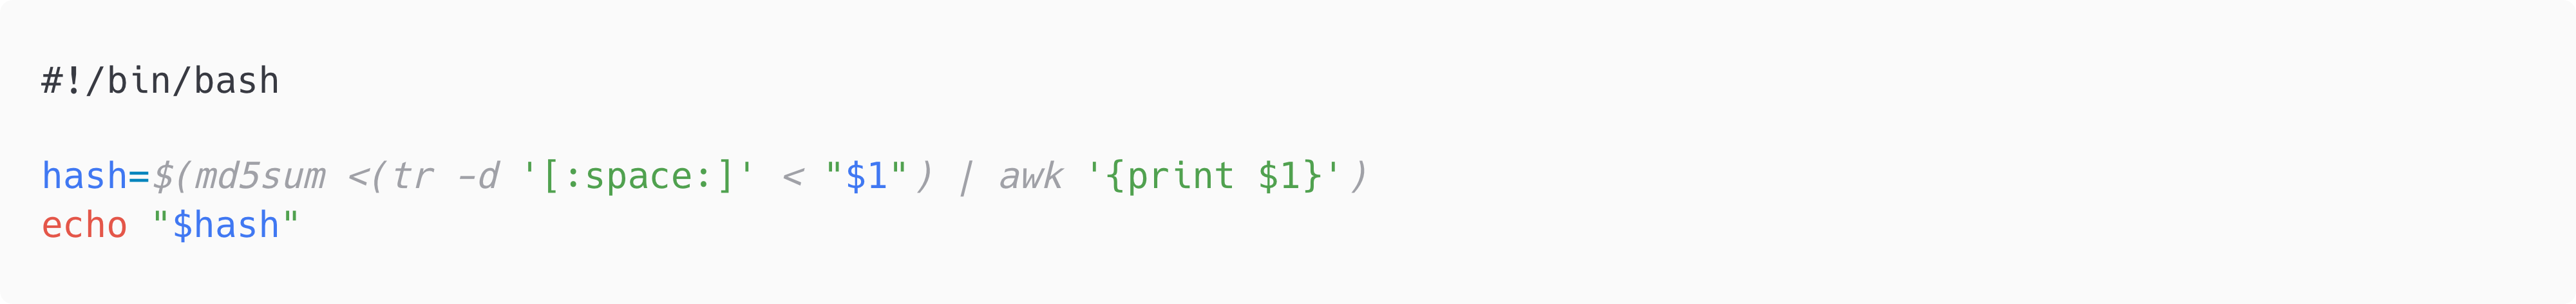
\includegraphics[width=12cm]{graphs/md5er.png}
\end{center}

\subsection{ formater.sh }

修改 .out 以及 .ans 的格式:

\begin{center}
	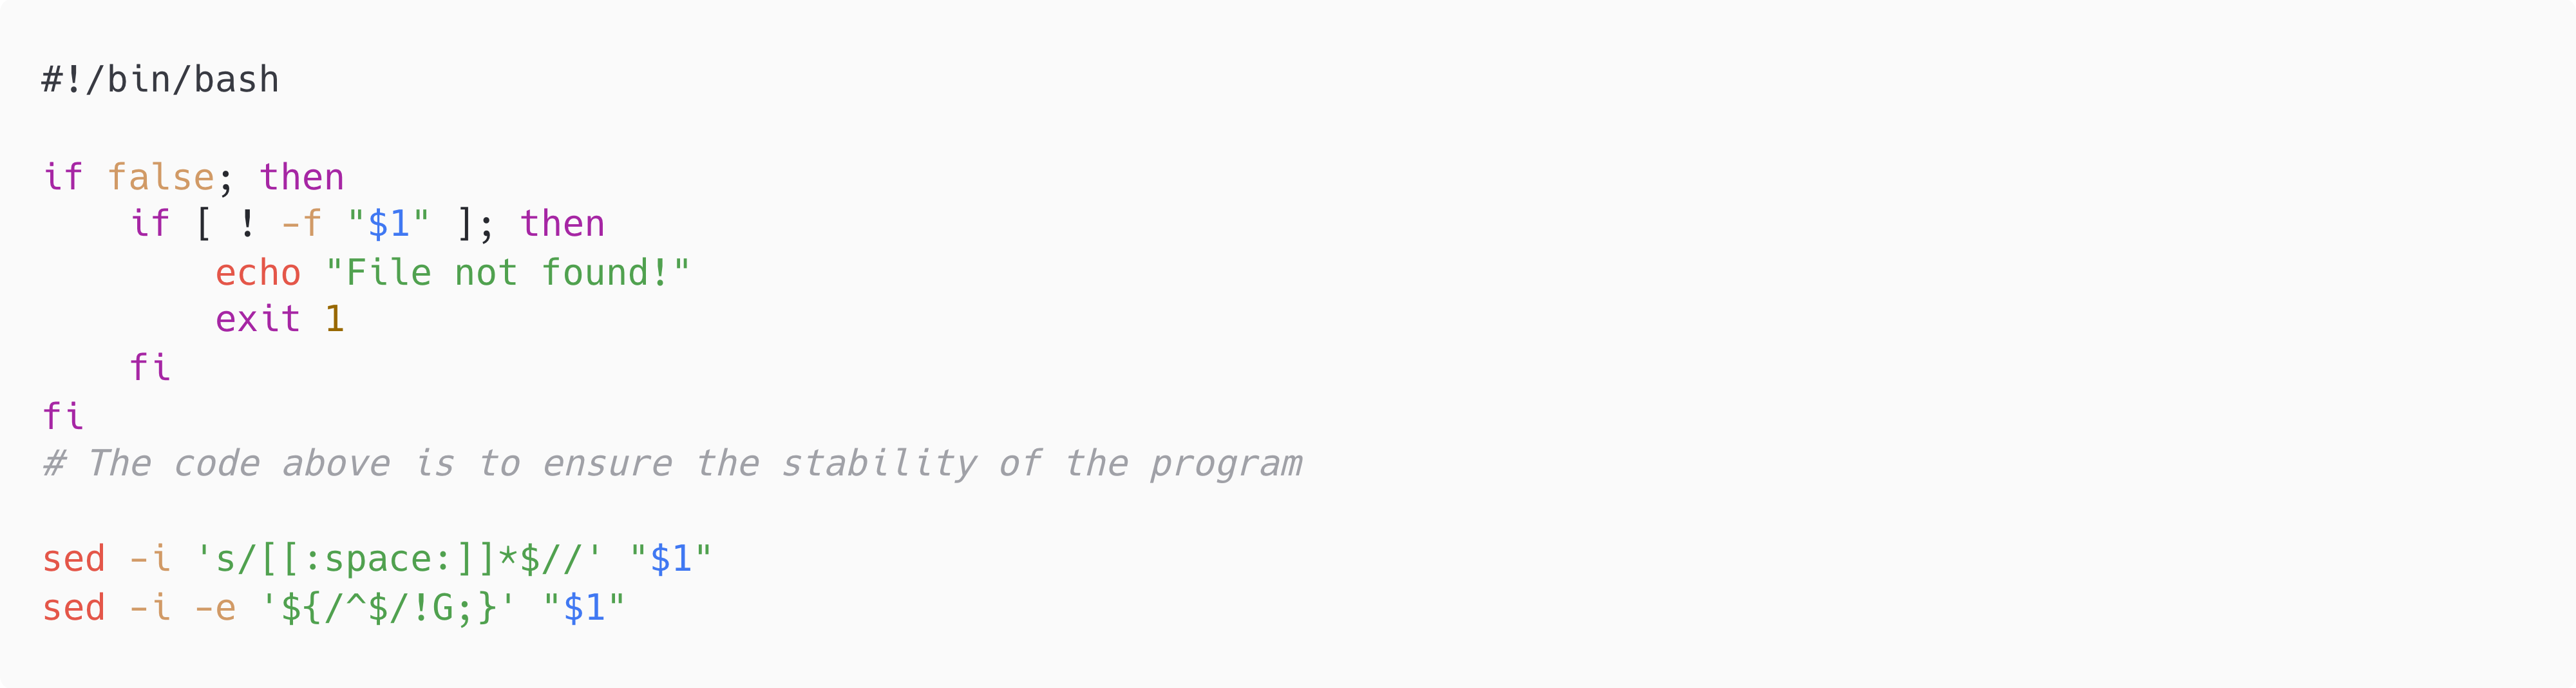
\includegraphics[width=12cm]{graphs/formater.png}
\end{center}

\subsection{ checker.sh }
对一份代码跑所有测试样例并比对.

\begin{lstlisting}[
basicstyle=\consolas
]
#!/bin/bash

# current=${pwd}
cd "$1"

g++ -o main -O2 -std=c++17 -DLOCAL main.cpp -ftrapv -fsanitize=address,undefined
for input in *.in; do 
    output=${input%.*}.out
    answer=${input%.*}.ans
    
    ./main < $input > $output

    echo "case ${input%.*}: "
    echo "My: "
    cat $output
    echo "Answer: "
    cat $answer

done
\end{lstlisting}

\newpage
\section{ data structure }

\subsection{ stack }
\begin{lstlisting}[style=cpp]
vi stk;
for (int i = 1; i <= n; i++){
    while (!stk.empty() and stk.back() > a[i]) {
        stk.pop_back();
    }
    stk.pop_back(a[i]);
}
\end{lstlisting}

\subsection{ queue }
\begin{lstlisting}[style=cpp]
std::deque<int> q;
for (int i = 1; i <= n; i++) {    
    while (!q.empty and a[q.back()] >= a[i]) p.pop_back();
    if (!q.empty() and i - q.front() >= k) q.pop_front();
    q.push_back(i);
}
\end{lstlisting}

\subsection{ DSU }
\begin{lstlisting}[style=cpp]
vi fa(n + 1);
std::iota(all(fa), 0);
std::function<void(int)> find = [&] (int x) -> int{
    return x == fa[x] ? x : fa[x] = find(fa[x]);
};
auto merge = [&] (int x, int y) -> void{
    x = find(x), y = find(y);
    if (x == y) return;
    /* operations */
    fa[y] = x;
};
\end{lstlisting}

\subsection{ ST }

用于解决可重复问题的数据结构。

可重复问题是指对运算 $opt$,满足 $x \ opt \ x = x$。

\subsubsection*{ 一维 }
\begin{lstlisting}[style=cpp]
vvi f(n + 1, vi(30));
vi Log2(n + 1);
auto ST_init = [&]() -> void {
    for (int i = 1; i <= n; i++) {
        f[i][0] = a[i];
        if (i > 1) Log2[i] = Log2[i / 2] + 1;
    };
    int t = Log2[n];
    for (int j = 1; j <= t; j++) {
        for (int i = 1; i <= n - (1 << j) + 1; i++) {
            f[i][j] = std::max(f[i][j - 1], f[i + (1 << (j - 1))][j - 1]);
        }
    }
};

auto ST_query = [&](int l, int r) -> int {
    int t = Log2[r - l + 1];
    return std::max(f[l][t], f[r - (1 << t) + 1][t]);
};
\end{lstlisting}

\subsubsection*{ 二维 }
\begin{lstlisting}[style=cpp]
std::vector f(n + 1, std::vector<std::array<std::array<int, 30>, 30>>(m + 1));
vi Log2(n + 1);
auto ST_init = [&]() -> void {
    for (int i = 2; i <= std::max(n, m); i++) {
        Log2[i] = Log2[i / 2] + 1;
    }
    for (int i = 2; i <= n; i++) {
        for (int j = 2; j <= m; j++) {
            f[i][j][0][0] = a[i][j];
        }
    }
    for (int ki = 0; ki <= Log2[n]; ki++) {
        for (int kj = 0; kj <= Log2[n]; kj++) {
            if (!ki && !kj) continue;
            for (int i = 1; i <= n - (1 << ki) + 1; i++) {
                for (int j = 1; j <= m - (1 << kj) + 1; j++) {
                    if (ki) {
                        f[i][j][ki][kj] =
                            std::max(f[i][j][ki - 1][kj], f[i + (1 << (ki - 1))][j][ki - 1][kj]);
                    } else {
                        f[i][j][ki][kj] =
                            std::max(f[i][j][ki][kj - 1], f[i][j + (1 << (kj - 1))][ki][kj - 1]);
                    }
                }
            }
        }
    }
};
auto ST_query = [&](int x1, int y1, int x2, int y2) -> int {
    int ki = Log2[x2 - x1 + 1], kj = Log2[y2 - y1 + 1];
    int t1 = f[x1][y1][ki][kj];
    int t2 = f[x2 - (1 << ki) + 1][y1][ki][kj];
    int t3 = f[x1][y2 - (1 << kj) + 1][ki][kj];
    int t4 = f[x2 - (1 << ki) + 1][y2 - (1 << kj) + 1][ki][kj];
    return std::max({t1, t2, t3, t4});
};
\end{lstlisting}

\subsection{ cartesian tree }
一种特殊的平衡树,用元素的值作为平衡点节点的 $val$,元素的下标作为 $key$。

\begin{lstlisting}[style=cpp]
// cartesian tree //
vi ls(n + 1), rs(n + 1), stk(n + 1);
int top = 1;
for (int i = 1; i <= n; i++) {
    int k = top;
    while (k and a[stk[k]] > a[i]) k--;
    if (k) rs[stk[k]] = i;
    if (k < top) ls[i] = stk[k + 1];
    stk[++k] = i;
    top = k;
}
\end{lstlisting}

\subsection{ segment tree }
\subsubsection*{ 维护半群 }
\begin{lstlisting}[style=cpp]
struct Info {
    /* 重载 operator+ */
};

struct Tag {
    /* 重载 operator== */
};

void infoApply(Info& a, int l, int r, const Tag& tag) {}

void tagApply(Tag& a, int l, int r, const Tag& tag) {}

template <class Info, class Tag>
class segTree {
#define ls i << 1
#define rs i << 1 | 1
#define mid ((l + r) >> 1)
#define lson ls, l, mid
#define rson rs, mid + 1, r

    int n;
    std::vector<Info> info;
    std::vector<Tag> tag;

    public:
    segTree(const std::vector<Info>& init) : n(init.size() - 1) {
        assert(n > 0);
        info.resize(4 << std::__lg(n));
        tag.resize(4 << std::__lg(n));
        auto build = [&](auto dfs, int i, int l, int r) {
            if (l == r) {
                info[i] = init[l];
                return;
            }
            dfs(dfs, lson);
            dfs(dfs, rson);
            push_up(i);
        };
        build(build, 1, 1, n);
    }


    private:
    void push_up(int i) { info[i] = info[ls] + info[rs]; }


    template <class... T>
    void apply(int i, int l, int r, const T&... val) {
        ::infoApply(info[i], l, r, val...);
        ::tagApply(tag[i], l, r, val...);
    }

    void push_down(int i, int l, int r) {
        if (tag[i] == Tag{}) return;
        apply(lson, tag[i]);
        apply(rson, tag[i]);
        tag[i] = {};
    }

    public:
    template <class... T>
    void rangeApply(int ql, int qr, const T&... val) {
        auto dfs = [&](auto dfs, int i, int l, int r) {
            if (qr < l or r < ql) return;
            if (ql <= l and r <= qr) {
                apply(i, l, r, val...);
                return;
            }
            push_down(i, l, r);
            dfs(dfs, lson);
            dfs(dfs, rson);
            push_up(i);
        };
        dfs(dfs, 1, 1, n);
    }

    Info rangeAsk(int ql, int qr) {
        Info res{};
        auto dfs = [&](auto dfs, int i, int l, int r) {
            if (qr < l or r < ql) return;
            if (ql <= l and r <= qr) {
                res = res + info[i];
                return;
            }
            push_down(i, l, r);
            dfs(dfs, lson);
            dfs(dfs, rson);
        };
        dfs(dfs, 1, 1, n);
        return res;
    }

#undef rson
#undef lson
#undef mid
#undef rs
#undef ls
};
\end{lstlisting}

\subsubsection*{ 区间修改 (带 add 和 mul 的 lazy tag) }

n 个数, m 次操作,操作分为

1. \(1 \ x \ y \ k\): 将区间 \([x, \ y]\) 中的数每个乘以 \(k\).
2. \(2 \ x \ y \ k\): 将区间 \([x, \ y]\) 中的数每个加上 \(k\).
3. \(3 \ x \ y\): 输出区间 \([x, \ y]\) 中数的和. (对 \(p\) 取模)

\begin{lstlisting}[style=cpp]
// Problem: P3373 【模板】线段树 2

struct Info {
    LL sum = 0;

    Info(LL _sum = 0) : sum(_sum) {}

    Info operator+(const Info& b) const { return Info(add(sum + b.sum)); }
};

struct Tag {
    LL add = 0, mul = 1;

    Tag(LL _add = 0, LL _mul = 1) : add(_add), mul(_mul) {}

    bool operator==(const Tag& b) const { return add == b.add and mul == b.mul; }
};

void infoApply(Info& a, int l, int r, const Tag& tag) {
    a.sum = add(mul(a.sum, tag.mul), mul((r - l + 1), tag.add));
}

void tagApply(Tag& a, int l, int r, const Tag& tag) {
    a.add = add(mul(a.add, tag.mul), tag.add);
    a.mul = mul(a.mul, tag.mul);
}

template <class Info, class Tag>
class segTree {
#define ls i << 1
#define rs i << 1 | 1
#define mid ((l + r) >> 1)
#define lson ls, l, mid
#define rson rs, mid + 1, r

    int n;
    std::vector<Info> info;
    std::vector<Tag> tag;

   public:
    segTree(const std::vector<Info>& init) : n(init.size() - 1) {
        assert(n > 0);
        info.resize(4 << std::__lg(n));
        tag.resize(4 << std::__lg(n));
        auto build = [&](auto dfs, int i, int l, int r) {
            if (l == r) {
                info[i] = init[l];
                return;
            }
            dfs(dfs, lson);
            dfs(dfs, rson);
            push_up(i);
        };
        build(build, 1, 1, n);
    }


   private:
    void push_up(int i) { info[i] = info[ls] + info[rs]; }


    template <class... T>
    void apply(int i, int l, int r, const T&... val) {
        ::infoApply(info[i], l, r, val...);
        ::tagApply(tag[i], l, r, val...);
    }

    void push_down(int i, int l, int r) {
        if (tag[i] == Tag{}) return;
        apply(lson, tag[i]);
        apply(rson, tag[i]);
        tag[i] = {};
    }

   public:
    template <class... T>
    void rangeMerge(int ql, int qr, const T&... val) {
        auto dfs = [&](auto dfs, int i, int l, int r) {
            if (qr < l or r < ql) return;
            if (ql <= l and r <= qr) {
                apply(i, l, r, val...);
                return;
            }
            push_down(i, l, r);
            dfs(dfs, lson);
            dfs(dfs, rson);
            push_up(i);
        };
        dfs(dfs, 1, 1, n);
    }

    Info rangeQuery(int ql, int qr) {
        Info res{};
        auto dfs = [&](auto dfs, int i, int l, int r) {
            if (qr < l or r < ql) return;
            if (ql <= l and r <= qr) {
                res = res + info[i];
                return;
            }
            push_down(i, l, r);
            dfs(dfs, lson);
            dfs(dfs, rson);
        };
        dfs(dfs, 1, 1, n);
        return res;
    }

#undef rson
#undef lson
#undef mid
#undef rs
#undef ls
};

int main() {
    std::ios::sync_with_stdio(false);
    std::cin.tie(0);
    std::cout.tie(0);

    int n, m, p;
    std::cin >> n >> m >> p;
    std::vector<Info> a(n + 1);
    for (int i = 1; i <= n; i++) std::cin >> a[i].sum;
    static segTree<Info, Tag> tr(a);

    while (m--) {
        int op, k, l, r;
        std::cin >> op >> l >> r;
        if (op == 1) {
            std::cin >> k;
            tr.rangeMerge(l, r, Tag(0, k));
        } else if (op == 2) {
            std::cin >> k;
            tr.rangeMerge(l, r, Tag(k, 1));
        } else {
            std::cout << tr.rangeQuery(l, r).sum << '\n';
        }
    }

    return 0;
}
\end{lstlisting}

\subsubsection*{ 动态开点权值线段树 }

如果要实现 push up 记得先开点再 push.

\begin{lstlisting}[style=cpp]
// Problem: P3369 【模板】普通平衡树

struct node {
    int id, l, r;
    int ls, rs;
    int sum;

    node(int _id, int _l, int _r) : id(_id), l(_l), r(_r) {
        ls = rs = 0;
        sum = 0;
    }
};


// Segment tree //
int idx = 1;
std::vector<node> tree = {node{0, 0, 0}};

auto new_node = [&](int l, int r) -> int {
    tree.push_back(node(idx, l, r));
    return idx++;
};

auto push_up = [&](int u) -> void {
    tree[u].sum = 0;
    if (tree[u].ls) tree[u].sum += tree[tree[u].ls].sum;
    if (tree[u].rs) tree[u].sum += tree[tree[u].rs].sum;
};

auto build = [&]() { new_node(-10000000, 10000000); };

std::function<void(int, int, int, int)> insert = [&](int u, int l, int r, int x) {
    if (l == r) {
        tree[u].sum++;
        return;
    }
    int mid = (l + r - 1) / 2;
    if (x <= mid) {
        if (!tree[u].ls) tree[u].ls = new_node(l, mid);
        insert(tree[u].ls, l, mid, x);
    } else {
        if (!tree[u].rs) tree[u].rs = new_node(mid + 1, r);
        insert(tree[u].rs, mid + 1, r, x);
    }
    push_up(u);
};

std::function<void(int, int, int, int)> remove = [&](int u, int l, int r, int x) {
    if (l == r) {
        if (tree[u].sum) tree[u].sum--;
        return;
    }
    int mid = (l + r - 1) / 2;
    if (x <= mid) {
        if (!tree[u].ls) return;
        remove(tree[u].ls, l, mid, x);
    } else {
        if (!tree[u].rs) return;
        remove(tree[u].rs, mid + 1, r, x);
    }
    push_up(u);
};

std::function<int(int, int, int, int)> get_rank_by_key = [&](int u, int l, int r, int x) -> int {
    if (l == r) {
        return 1;
    }
    int mid = (l + r - 1) / 2;
    int ans = 0;
    if (x <= mid) {
        if (!tree[u].ls) return 1;
        ans = get_rank_by_key(tree[u].ls, l, mid, x);
    } else {
        if (!tree[u].rs) return tree[tree[u].ls].sum + 1;
        if (!tree[u].ls) {
            ans = get_rank_by_key(tree[u].rs, mid + 1, r, x);
        } else {
            ans = get_rank_by_key(tree[u].rs, mid + 1, r, x) + tree[tree[u].ls].sum;
        }
    }
    return ans;
};

std::function<int(int, int, int, int)> get_key_by_rank = [&](int u, int l, int r, int x) -> int {
    if (l == r) {
        return l;
    }
    int mid = (l + r - 1) / 2;
    if (tree[u].ls) {
        if (x <= tree[tree[u].ls].sum) {
            return get_key_by_rank(tree[u].ls, l, mid, x);
        } else {
            return get_key_by_rank(tree[u].rs, mid + 1, r, x - tree[tree[u].ls].sum);
        }
    } else {
        return get_key_by_rank(tree[u].rs, mid + 1, r, x);
    }
};

std::function<int(int)> get_prev = [&](int x) -> int {
    int rank = get_rank_by_key(1, -10000000, 10000000, x) - 1;
    debug(rank);
    return get_key_by_rank(1, -10000000, 10000000, rank);
};

std::function<int(int)> get_next = [&](int x) -> int {
    debug(x + 1);
    int rank = get_rank_by_key(1, -10000000, 10000000, x + 1);
    debug(rank);
    return get_key_by_rank(1, -10000000, 10000000, rank);
};
\end{lstlisting}

\subsubsection*{ 线段树上二分 }
\begin{lstlisting}[style=cpp]
int lc[M], rc[M], w[M], tot;
ll a[N];
void ins(int& o, ll l, ll r, ll x) {
    if (!o) o = ++tot;
    ++w[o];
    if (l == r) return ;
    ll md = l + r >> 1;
    if (x <= md) ins(lc[o], l, md, x);
    else ins(rc[o], md + 1, r, x);
};
int ask(int o, ll L, ll R, ll l, ll r) {
    if (!o) return 0;
    // assert(o);
    if (l <= L && R <= r) return w[o];
    ll md = L + R >> 1; int z = 0;
    if (r >= L) z += ask(lc[o], L, md, l, r);
    if (l < R) z += ask(rc[o], md + 1, R, l, r);
    return z;
};
auto bs(int o, ll l, ll r, int k) {
    // assert(k <= w[o]);
    if (l == r) return std::make_pair(l, w[o] - k);
    ll md = l + r >> 1;
    if (w[rc[o]] >= k) return bs(rc[o], md + 1, r, k);
    else return bs(lc[o], l, md, k - w[rc[o]]);
};
\end{lstlisting}


\subsubsection*{ (权值) 线段树合并分裂 }
首先村落里的一共有 \(n\) 座房屋, 并形成一个树状结构. 然后救济粮分 \(m\) 次发放, 每次选择两个房屋 \((x,y)\), 然后对于 \(x\) 到 \(y\) 的路径上每座房子里发放一袋 \(z\) 类型的救济粮.
查询所有的救济粮发放完毕后, 每座房子里存放的最多的是哪种救济粮.

\begin{lstlisting}[style=cpp]
// Problem: P4556 [Vani有约会]雨天的尾巴 /【模板】线段树合并

struct node {
    int l, r, id;
    int ls, rs;
    int cnt, ans;

    node(int _id, int _l, int _r) : id(_id), l(_l), r(_r) {
        ls = rs = 0;
        cnt = ans = 0;
    }
};

int main() {
    std::ios::sync_with_stdio(false);
    std::cin.tie(0);
    std::cout.tie(0);

    int n, m;
    std::cin >> n >> m;
    vvi e(n + 1);
    vi ans(n + 1);
    for (int i = 1; i < n; i++) {
        int u, v;
        std::cin >> u >> v;
        e[u].push_back(v);
        e[v].push_back(u);
    }

    /* Segment tree */
    int idx = 1;
    vi rt(n + 1);
    std::vector<node> tree = {node{0, 0, 0}};

    auto new_node = [&](int l, int r) -> int {
        tree.push_back(node(idx, l, r));
        return idx++;
    };

    auto push_up = [&](int u) -> void {
        if (!tree[u].ls) {
            tree[u].cnt = tree[tree[u].rs].cnt;
            tree[u].ans = tree[tree[u].rs].ans;
        } else if (!tree[u].rs) {
            tree[u].cnt = tree[tree[u].ls].cnt;
            tree[u].ans = tree[tree[u].ls].ans;
        } else {
            if (tree[tree[u].rs].cnt > tree[tree[u].ls].cnt) {
                tree[u].cnt = tree[tree[u].rs].cnt;
                tree[u].ans = tree[tree[u].rs].ans;
            } else {
                tree[u].cnt = tree[tree[u].ls].cnt;
                tree[u].ans = tree[tree[u].ls].ans;
            }
        }
    };

    std::function<void(int, int, int, int, int)> modify = [&](int u, int l, int r, int x, int k) {
        if (l == r) {
            tree[u].cnt += k;
            tree[u].ans = l;
            return;
        }
        int mid = (l + r) >> 1;
        if (x <= mid) {
            if (!tree[u].ls) tree[u].ls = new_node(l, mid);
            modify(tree[u].ls, l, mid, x, k);
        } else {
            if (!tree[u].rs) tree[u].rs = new_node(mid + 1, r);
            modify(tree[u].rs, mid + 1, r, x, k);
        }
        push_up(u);
    };

    std::function<int(int, int, int, int)> merge = [&](int u, int v, int l, int r) -> int {
        /* v 的信息传递给 u */
        if (!u) return v;
        if (!v) return u;
        if (l == r) {
            tree[u].cnt += tree[v].cnt;
            return u;
        }
        int mid = (l + r) >> 1;
        tree[u].ls = merge(tree[u].ls, tree[v].ls, l, mid);
        tree[u].rs = merge(tree[u].rs, tree[v].rs, mid + 1, r);
        push_up(u);
        return u;
    };

    /* LCA */

    for (int i = 1; i <= n; i++) {
        rt[i] = idx;
        new_node(1, 100000);
    }

    for (int i = 1; i <= m; i++) {
        int u, v, w;
        std::cin >> u >> v >> w;
        int lca = LCA(u, v);
        modify(rt[u], 1, 100000, w, 1);
        modify(rt[v], 1, 100000, w, 1);
        modify(rt[lca], 1, 100000, w, -1);
        if (father[lca][0]) {
            modify(rt[father[lca][0]], 1, 100000, w, -1);
        }
    }

    /* dfs */
    std::function<void(int, int)> Dfs = [&](int u, int fa) {
        for (auto v : e[u]) {
            if (v == fa) continue;
            Dfs(v, u);
            merge(rt[u], rt[v], 1, 100000);
        }
        ans[u] = tree[rt[u]].ans;
        if (tree[rt[u]].cnt == 0) ans[u] = 0;
    };

    Dfs(1, 0);

    for (int i = 1; i <= n; i++) {
        std::cout << ans[i] << '\n';
    }

    return 0;
}
\end{lstlisting}

\begin{lstlisting}[style=cpp]
#include<bits/stdc++.h>
using namespace std;
namespace Acc{
    using i64=int64_t;
    enum{N=200009,M=10000000};
    i64 v[M];
    int lc[M],rc[M],tot,a[N],r[N];
    auto up=[](int o){
        v[o]=v[lc[o]]+v[rc[o]];
    };
    void bd(int&o,int l,int r){
        if(o=++tot,l==r)return cin>>v[o],void();
        int md=l+r>>1;
        bd(lc[o],l,md),bd(rc[o],md+1,r),up(o);
    }
    void spl(int&o,int&x,int l,int r,int L,int R){
        if(l<=L&&R<=r)return o=x,x=0,void();
        int md=L+R>>1;
        o=++tot;
        if(l<=md)spl(lc[o],lc[x],l,r,L,md);
        if(r>md)spl(rc[o],rc[x],l,r,md+1,R);
        up(o),up(x);
    }
    void mg(int&o,int x,int l,int r){
        if(!o||!x)return o|=x,void();
        if(l==r)return v[o]+=v[x],void();
        int md=l+r>>1;
        mg(lc[o],lc[x],l,md);
        mg(rc[o],rc[x],md+1,r);
        up(o);
    }
    void ins(int&o,int l,int r,int x,int k){
        if(!o)o=++tot;
        if(v[o]+=k,l==r)return;
        int md=l+r>>1;
        x<=md?ins(lc[o],l,md,x,k):ins(rc[o],md+1,r,x,k);
    }
    i64 qry(int o,int l,int r,int L,int R){
        if(!o)return 0;
        if(l<=L&&R<=r)return v[o];
        int md=L+R>>1;i64 z=0;
        if(l<=md)z=qry(lc[o],l,r,L,md);
        if(r>md)z+=qry(rc[o],l,r,md+1,R);
        return z;
    }
    int kth(int o,int l,int r,int k){
        if(l==r)return l;
        if(k>v[o])return -1;
        int md=l+r>>1;
        if(k<=v[lc[o]])return kth(lc[o],l,md,k);
        else return kth(rc[o],md+1,r,k-v[lc[o]]);
    }
    auto work=[](){
        int n,m,i,x,y,o=1;
        for(cin>>n>>m,bd(r[1],1,n);m--;)switch(cin>>i,i){
            case 0:cin>>i>>x>>y,spl(r[++o],r[i],x,y,1,n);break;
            case 1:cin>>x>>y,mg(r[x],r[y],1,n);break;
            case 2:cin>>i>>x>>y,ins(r[i],1,n,y,x);break;
            case 3:cin>>i>>x>>y,cout<<qry(r[i],x,y,1,n)<<'\n';break;
            case 4:cin>>i>>x,cout<<kth(r[i],1,n,x)<<'\n';break;
        }
    };
}
int main(){
    ios::sync_with_stdio(0);
    cin.tie(0),Acc::work();
}
\end{lstlisting}

\subsection{ hjt segment tree }

\subsubsection*{ 第 1 个例题 }

\(n\) 个数, \(m\) 次操作, 操作分别为

\begin{enumerate}
	\item $v_i \ 1 \ loc_i \ value_i$: 将第 $v_i$ 个版本的 $a[loc_i]$ 修改为 $value_i$,
	\item $v_i \ 2 \ loc_i$: 拷贝第 $v_i$ 个版本, 并查询该版本的 $a[loc_i]$.
\end{enumerate}

\begin{lstlisting}[style=cpp]
// 洛谷 P3919 【模板】可持久化线段树 1(可持久化数组)

struct node {
    int l, r, key;
};

int main() {
    std::ios::sync_with_stdio(false);
    std::cin.tie(0);
    std::cout.tie(0);

    int n, m;
    std::cin >> n >> m;
    vi a(n + 1);
    for (int i = 1; i <= n; i++) {
        std::cin >> a[i];
    }

    /* hjt segment tree */
    int idx = 0;
    vi root(m + 1);
    std::vector<node> tr(n * 25);

    std::function<int(int, int)> build = [&](int l, int r) -> int {
        int p = ++idx;
        if (l == r) {
            tr[p].key = a[l];
            return p;
        }
        int mid = (l + r) >> 1;
        tr[p].l = build(l, mid);
        tr[p].r = build(mid + 1, r);
        return p;
    };

    std::function<int(int, int, int, int, int)> modify = [&](int p, int l, int r, int k,
                                                             int x) -> int {
        int q = ++idx;
        tr[q].l = tr[p].l, tr[q].r = tr[p].r;
        if (tr[q].l == tr[q].r) {
            tr[q].key = x;
            return q;
        }
        int mid = (l + r) >> 1;
        if (k <= mid) {
            tr[q].l = modify(tr[q].l, l, mid, k, x);
        } else {
            tr[q].r = modify(tr[q].r, mid + 1, r, k, x);
        }
        return q;
    };

    std::function<int(int, int, int, int)> query = [&](int p, int l, int r, int k) -> int {
        if (tr[p].l == tr[p].r) {
            return tr[p].key;
        }
        int mid = (l + r) >> 1;
        if (k <= mid) {
            return query(tr[p].l, l, mid, k);
        } else {
            return query(tr[p].r, mid + 1, r, k);
        }
    };

    root[0] = build(1, n);

    for (int i = 1; i <= m; i++) {
        int op, ver, k, x;
        std::cin >> ver >> op;
        if (op == 1) {
            std::cin >> k >> x;
            root[i] = modify(root[ver], 1, n, k, x);
        } else {
            std::cin >> k;
            root[i] = root[ver];
            std::cout << query(root[ver], 1, n, k) << '\n';
        }
    }

    return 0;
}
\end{lstlisting}

\subsubsection*{ 第 2 个例题 }

长度为 $n$ 的序列 $a$, $m$ 次查询, 每次查询 $[l, r]$ 中的第 $k$ 小值.

\begin{lstlisting}[style=cpp]
// 洛谷P3834 【模板】可持久化线段树 2

struct node {
    int l, r, cnt;
};

int main() {
    std::ios::sync_with_stdio(false);
    std::cin.tie(0);
    std::cout.tie(0);

    int n, m;
    std::cin >> n >> m;
    vi a(n + 1), v;
    for (int i = 1; i <= n; i++) {
        std::cin >> a[i];
        v.push_back(a[i]);
    }
    std::sort(all(v));
    v.erase(unique(all(v)), v.end());
    auto find = [&](int x) -> int { return std::lower_bound(all(v), x) - v.begin() + 1; };

    /* hjt segment tree */
    std::vector<node>(n * 25);
    vi root(n + 1);
    int idx = 0;

    std::function<int(int, int)> build = [&](int l, int r) -> int {
        int p = ++idx;
        if (l == r) return p;
        int mid = (l + r) >> 1;
        tr[p].l = build(l, mid), tr[p].r = build(mid + 1, r);
        return p;
    };

    std::function<int(int, int, int, int)> modify = [&](int p, int l, int r, int x) -> int {
        int q = ++idx;
        tr[q] = tr[p];
        if (tr[q].l == tr[q].r) {
            tr[q].cnt++;
            return q;
        }
        int mid = (l + r) >> 1;
        if (x <= mid) {
            tr[q].l = modify(tr[q].l, l, mid, x);
        } else {
            tr[q].r = modify(tr[q].r, mid + 1, r, x);
        }
        tr[q].cnt = tr[tr[q].l].cnt + tr[tr[q].r].cnt;
        return q;
    };

    std::function<int(int, int, int, int, int)> query = [&](int p, int q, int l, int r,
                                                            int x) -> int {
        if (l == r) return l;
        int cnt = tr[tr[p].l].cnt - tr[tr[q].l].cnt;
        int mid = (l + r) >> 1;
        if (x <= cnt) {
            return query(tr[p].l, tr[q].l, l, mid, x);
        } else {
            return query(tr[p].r, tr[q].r, mid + 1, r, x - cnt);
        }
    };

    root[0] = build(1, v.size());


    for (int i = 1; i <= n; i++) {
        root[i] = modify(root[i - 1], 1, v.size(), find(a[i]));
    }
    for (int i = 1; i <= m; i++) {
        int l, r, k;
        std::cin >> l >> r >> k;
        std::cout << v[query(root[r], root[l - 1], 1, v.size(), k) - 1] << '\n';
    }

    return 0;
}
\end{lstlisting}

\subsection{ LiChao Tree }

线段版本 

\begin{lstlisting}[style=cpp]
#include<bits/stdc++.h>
using namespace std;
namespace Acc{
#define lc (o<<1)
#define rc (o<<1|1)
    const int N = 4e5+10;
    int v[N],n,l,r,z;
    double k[N],b[N];
    inline void r1(int&x){x=(x+z-1)%39989+1;}
    inline void r2(int&x){x=(x+z-1)%1000000000+1;}
    double f(int o,int x){
        return k[o]*x+b[o];
    }
    int beat(int x,int a,int b){
        double u=f(a,x),v=f(b,x);
        return fabs(u-v)<=1e-8?a<b:u>v;
    }
    void add(int o,int L,int R,int x){
        int md=L+R>>1;
        if(l<=L&&R<=r){
            if(!v[o])return (void)(v[o]=x);
            if(beat(L,v[o],x) && beat(R,v[o],x))return;
            if(beat(L,x,v[o]) && beat(R,x,v[o]))return (void)(v[o]=x);
            if(beat(md,x,v[o]))swap(x,v[o]);
            if(beat(L,x,v[o]))add(lc,L,md,x);
            else add(rc,md+1,R,x);
            return;
        }
        if(r>md)add(rc,md+1,R,x);
        if(l<=md)add(lc,L,md,x);
    }
    int ask(int o,int L,int R){
        if(L==R)return v[o];
        int md=L+R>>1,h=l<=md?ask(lc,L,md):ask(rc,md+1,R);
        return beat(l,h,v[o])?h:v[o];
    }
    void work(){
        cin>>n;
        for(int op,y1,y2,c=0;n--;){
            cin>>op;
            if(op){
                cin>>l>>y1>>r>>y2,++c,r1(l),r2(y1),r1(r),r2(y2);
                if(l==r)k[c]=0,b[c]=max(y1,y2);
                else {
                    if(l>r)swap(l,r),swap(y1,y2);
                    k[c]=(y2-y1+0.)/(r-l),b[c]=y1-k[c]*l;
                }
                add(1,1,4e4+10,c);
            }else cin>>l,r1(l),cout<<(z=ask(1,1,4e4+10))<<'\n';
        }
    }
}
int main(){
    return Acc::work(),0;
}
\end{lstlisting}

\subsection{ treap }

\subsubsection*{ 旋转 treap }

$n$ 次操作, 操作分为如下 $6$ 种:
\begin{enumerate}
	\item 插入数 $x$,
	\item 删除数 $x$ (若有多个相同的数,只删除一个),
	\item 查询数 $x$ 的排名 (排名定义为小于 $x$ 的数的个数 $+$ $1$),
	\item 查询排名为 $x$ 的数,
	\item 求 $x$ 的前驱 (前驱定义为小于 $x$ 的最大数),
	\item 求 $x$ 的后继 (后继定义为大于 $x$ 的最小数).
\end{enumerate}

\begin{lstlisting}[style=cpp]
// Problem: P3369 【模板】普通平衡树

int n, root, idx;

struct node {
    int l, r;
    int key, val;
    int cnt, size;
} treap[N];

void push_up(int p) {
    treap[p].size = treap[treap[p].l].size + treap[treap[p].r].size + treap[p].cnt;
}

int get_node(int key) {
    treap[++idx].key = key;
    treap[idx].val = rand();
    treap[idx].cnt = treap[idx].size = 1;
    return idx;
}

void zig(int &p) {
    // 右旋 //
    int q = treap[p].l;
    treap[p].l = treap[q].r, treap[q].r = p, p = q;
    push_up(treap[p].r), push_up(p);
}

void zag(int &p) {
    // 左旋 //
    int q = treap[p].r;
    treap[p].r = treap[q].l, treap[q].l = p, p = q;
    push_up(treap[p].l), push_up(p);
}

void build() {
    get_node(-inf), get_node(inf);
    root = 1, treap[1].r = 2;
    push_up(root);
    if (treap[1].val < treap[2].val) zag(root);
}

void insert(int &p, int key) {
    if (!p) {
        p = get_node(key);
    } else if (treap[p].key == key) {
        treap[p].cnt++;
    } else if (treap[p].key > key) {
        insert(treap[p].l, key);
        if (treap[treap[p].l].val > treap[p].val) zig(p);
    } else {
        insert(treap[p].r, key);
        if (treap[treap[p].r].val > treap[p].val) zag(p);
    }
    push_up(p);
}

void remove(int &p, int key) {
    if (!p) return;
    if (treap[p].key == key) {
        if (treap[p].cnt > 1) {
            treap[p].cnt--;
        } else if (treap[p].l || treap[p].r) {
            if (!treap[p].r || treap[treap[p].l].val > treap[treap[p].r].val) {
                zig(p);
                remove(treap[p].r, key);
            } else {
                zag(p);
                remove(treap[p].l, key);
            }
        } else {
            p = 0;
        }
    } else if {
        (treap[p].key > key) remove(treap[p].l, key);
    } else {
        remove(treap[p].r, key);
    }
    push_up(p);
}

int get_rank_by_key(int p, int key) {
    // 通过数值找排名 //
    if (!p) return 0;
    if (treap[p].key == key) return treap[treap[p].l].size;
    if (treap[p].key > key) return get_rank_by_key(treap[p].l, key);
    return treap[treap[p].l].size + treap[p].cnt + get_rank_by_key(treap[p].r, key);
}

int get_key_by_rank(int p, int rank) {
    // 通过排名找数值 //
    if (!p) return inf;
    if (treap[treap[p].l].size >= rank) return get_key_by_rank(treap[p].l, rank);
    if (treap[treap[p].l].size + treap[p].cnt >= rank) return treap[p].key;
    return get_key_by_rank(treap[p].r, rank - treap[treap[p].l].size - treap[p].cnt);
}

int get_prev(int p, int key) {
    // 找前驱 //
    if (!p) return -inf;
    if (treap[p].key >= key) return get_prev(treap[p].l, key);
    return max(treap[p].key, get_prev(treap[p].r, key));
}

int get_next(int p, int key) {
    // 找后继 //
    if (!p) return inf;
    if (treap[p].key <= key) return get_next(treap[p].r, key);
    return min(treap[p].key, get_next(treap[p].l, key));
}

int main() {
    ios::sync_with_stdio(false);
    cin.tie(0);
    cout.tie(0);

    cin >> n;
    build();
    rep(i, 1, n) {
        int op, x;
        cin >> op >> x;
        if (op == 1) {
            insert(root, x);
        } else if (op == 2) {
            remove(root, x);
        } else if (op == 3) {
            cout << get_rank_by_key(root, x) << '\n';
        } else if (op == 4) {
            cout << get_key_by_rank(root, x + 1) << '\n';
        } else if (op == 5) {
            cout << get_prev(root, x) << '\n';
        } else {
            cout << get_next(root, x) << '\n';
        }
    }
    return 0;
}
\end{lstlisting}

\subsubsection*{ 无旋 treap }

与旋转 Treap 同一个题目

\begin{lstlisting}[style=cpp]
struct node {
    node *ch[2];
    int key, val;
    int cnt, size;

    node(int _key) : key(_key), cnt(1), size(1) {
        ch[0] = ch[1] = nullptr;
        val = rand();
    }

    // node(node *_node) {
    // key = _node->key, val = _node->val, cnt = _node->cnt, size = _node->size;
    // }

    inline void push_up() {
        size = cnt;
        if (ch[0] != nullptr) size += ch[0]->size;
        if (ch[1] != nullptr) size += ch[1]->size;
    }
};

struct treap {
#define _2 second.first
#define _3 second.second

    node *root;

    pair<node *, node *> split(node *p, int key) {
        if (p == nullptr) return {nullptr, nullptr};
        if (p->key <= key) {
            auto temp = split(p->ch[1], key);
            p->ch[1] = temp.first;
            p->push_up();
            return {p, temp.second};
        } else {
            auto temp = split(p->ch[0], key);
            p->ch[0] = temp.second;
            p->push_up();
            return {temp.first, p};
        }
    }

    pair<node *, pair<node *, node *> > split_by_rank(node *p, int rank) {
        if (p == nullptr) return {nullptr, {nullptr, nullptr}};
        int ls_size = p->ch[0] == nullptr ? 0 : p->ch[0]->size;
        if (rank <= ls_size) {
            auto temp = split_by_rank(p->ch[0], rank);
            p->ch[0] = temp._3;
            p->push_up();
            return {temp.first, {temp._2, p}};
        } else if (rank <= ls_size + p->cnt) {
            node *lt = p->ch[0];
            node *rt = p->ch[1];
            p->ch[0] = p->ch[1] = nullptr;
            return {lt, {p, rt}};
        } else {
            auto temp = split_by_rank(p->ch[1], rank - ls_size - p->cnt);
            p->ch[1] = temp.first;
            p->push_up();
            return {p, {temp._2, temp._3}};
        }
    }

    node *merge(node *u, node *v) {
        if (u == nullptr && v == nullptr) return nullptr;
        if (u != nullptr && v == nullptr) return u;
        if (v != nullptr && u == nullptr) return v;
        if (u->val < v->val) {
            u->ch[1] = merge(u->ch[1], v);
            u->push_up();
            return u;
        } else {
            v->ch[0] = merge(u, v->ch[0]);
            v->push_up();
            return v;
        }
    }

    void insert(int key) {
        auto temp = split(root, key);
        auto l_tr = split(temp.first, key - 1);
        node *new_node;
        if (l_tr.second == nullptr) {
            new_node = new node(key);
        } else {
            l_tr.second->cnt++;
            l_tr.second->push_up();
        }
        node *l_tr_combined = merge(l_tr.first, l_tr.second == nullptr ? new_node : l_tr.second);
        root = merge(l_tr_combined, temp.second);
    }

    void remove(int key) {
        auto temp = split(root, key);
        auto l_tr = split(temp.first, key - 1);
        if (l_tr.second->cnt > 1) {
            l_tr.second->cnt--;
            l_tr.second->push_up();
            l_tr.first = merge(l_tr.first, l_tr.second);
        } else {
            if (temp.first == l_tr.second) temp.first = nullptr;
            delete l_tr.second;
            l_tr.second = nullptr;
        }
        root = merge(l_tr.first, temp.second);
    }

    int get_rank_by_key(node *p, int key) {
        auto temp = split(p, key - 1);
        int ret = (temp.first == nullptr ? 0 : temp.first->size) + 1;
        root = merge(temp.first, temp.second);
        return ret;
    }

    int get_key_by_rank(node *p, int rank) {
        auto temp = split_by_rank(p, rank);
        int ret = temp._2->key;
        root = merge(temp.first, merge(temp._2, temp._3));
        return ret;
    }

    int get_prev(int key) {
        auto temp = split(root, key - 1);
        int ret = get_key_by_rank(temp.first, temp.first->size);
        root = merge(temp.first, temp.second);
        return ret;
    }

    int get_nex(int key) {
        auto temp = split(root, key);
        int ret = get_key_by_rank(temp.second, 1);
        root = merge(temp.first, temp.second);
        return ret;
    }
};

treap tr;

int main() {
    ios::sync_with_stdio(false);
    cin.tie(0);
    cout.tie(0);

    srand(time(0));

    int n;
    cin >> n;
    while (n--) {
        int op, x;
        cin >> op >> x;
        if (op == 1) {
            tr.insert(x);
        } else if (op == 2) {
            tr.remove(x);
        } else if (op == 3) {
            cout << tr.get_rank_by_key(tr.root, x) << '\n';
        } else if (op == 4) {
            cout << tr.get_key_by_rank(tr.root, x) << '\n';
        } else if (op == 5) {
            cout << tr.get_prev(x) << '\n';
        } else {
            cout << tr.get_nex(x) << '\n';
        }
    }
    return 0;
}
\end{lstlisting}

\subsubsection*{ 用 01 trie 实现的一种方式 }

同样的题目, 注意使用 01 trie 只能存在非负数.

速度能快不少, 但只能单点操作, 而且有点费空间.

\begin{lstlisting}[style=cpp]
// 洛谷 P3369 【模板】普通平衡树

struct Treap {
    int id = 1, maxlog = 25;
    int ch[N * 25][2], siz[N * 25];

    int newnode() {
        id++;
        ch[id][0] = ch[id][1] = siz[id] = 0;
        return id;
    }

    void merge(int key, int cnt) {
        int u = 1;
        for (int i = maxlog - 1; i >= 0; i--) {
            int v = (key >> i) & 1;
            if (!ch[u][v]) ch[u][v] = newnode();
            u = ch[u][v];
            siz[u] += cnt;
        }
    }

    int get_key_by_rank(int rank) {
        int u = 1, key = 0;
        for (int i = maxlog - 1; i >= 0; i--) {
            if (siz[ch[u][0]] >= rank) {
                u = ch[u][0];
            } else {
                key |= (1 << i);
                rank -= siz[ch[u][0]];
                u = ch[u][1];
            }
        }
        return key;
    }

    int get_rank_by_key(int rank) {
        int key = 0;
        int u = 1;
        for (int i = maxlog - 1; i >= 0; i--) {
            if ((rank >> i) & 1) {
                key += siz[ch[u][0]];
                u = ch[u][1];
            } else {
                u = ch[u][0];
            }
            if (!u) break;
        }
        return key;
    }

    int get_prev(int x) { return get_key_by_rank(get_rank_by_key(x)); }
    int get_next(int x) { return get_key_by_rank(get_rank_by_key(x + 1) + 1); }
} treap;

const int num = 1e7;
int n, op, x;

int main() {
    std::ios::sync_with_stdio(false);
    std::cin.tie(0);
    std::cout.tie(0);

    std::cin >> n;
    for (int i = 1; i <= n; i++) {
        std::cin >> op >> x;
        if (op == 1) {
            treap.merge(x + num, 1);
        } else if (op == 2) {
            treap.merge(x + num, -1);
        } else if (op == 3) {
            std::cout << treap.get_rank_by_key(x + num) + 1 << '\n';
        } else if (op == 4) {
            std::cout << treap.get_key_by_rank(x) - num << '\n';
        } else if (op == 5) {
            std::cout << treap.get_prev(x + num) - num << '\n';
        } else if (op == 6) {
            std::cout << treap.get_next(x + num) - num << '\n';
        }
    }
    return 0;
}
\end{lstlisting}

\subsection{ splay }

\subsubsection*{ 文艺平衡树 }

初始为 $1$ 到 $n$ 的序列, $m$ 次操作, 每次将序列下标为 $[l \sim r]$ 的区间翻转.

\begin{lstlisting}[style=cpp]
// 洛谷 P3391 【模板】文艺平衡树

struct node {
    int ch[2], fa, key;
    int siz, flag;

    void init(int _fa, int _key) { fa = _fa, key = _key, siz = 1; }
};

struct splay {
    node tr[N];
    int n, root, idx;

    bool get(int u) { return u == tr[tr[u].fa].ch[1]; }

    void pushup(int u) { tr[u].siz = tr[tr[u].ch[0]].siz + tr[tr[u].ch[1]].siz + 1; }

    void pushdown(int u) {
        if (tr[u].flag) {
            std::swap(tr[u].ch[0], tr[u].ch[1]);
            tr[tr[u].ch[0]].flag ^= 1, tr[tr[u].ch[1]].flag ^= 1;
            tr[u].flag = 0;
        }
    }

    void rotate(int x) {
        int y = tr[x].fa, z = tr[y].fa;
        int op = get(x);
        tr[y].ch[op] = tr[x].ch[op ^ 1];
        if (tr[x].ch[op ^ 1]) tr[tr[x].ch[op ^ 1]].fa = y;
        tr[x].ch[op ^ 1] = y;
        tr[y].fa = x, tr[x].fa = z;
        if (z) tr[z].ch[y == tr[z].ch[1]] = x;
        pushup(y), pushup(x);
    }

    void opt(int u, int k) {
        for (int f = tr[u].fa; f = tr[u].fa, f != k; rotate(u)) {
            if (tr[f].fa != k) rotate(get(u) == get(f) ? f : u);
        }
        if (k == 0) root = u;
    }

    void output(int u) {
        pushdown(u);
        if (tr[u].ch[0]) output(tr[u].ch[0]);
        if (tr[u].key >= 1 && tr[u].key <= n) {
            std::cout << tr[u].key << ' ';
        }
        if (tr[u].ch[1]) output(tr[u].ch[1]);
    }

    void insert(int key) {
        idx++;
        tr[idx].ch[0] = root;
        tr[idx].init(0, key);
        tr[root].fa = idx;
        root = idx;
        pushup(idx);
    }

    int kth(int k) {
        int u = root;
        while (1) {
            pushdown(u);
            if (tr[u].ch[0] && k <= tr[tr[u].ch[0]].siz) {
                u = tr[u].ch[0];
            } else {
                k -= tr[tr[u].ch[0]].siz + 1;
                if (k <= 0) {
                    opt(u, 0);
                    return u;
                } else {
                    u = tr[u].ch[1];
                }
            }
        }
    }

} splay;

int n, m, l, r;

int main() {
    std::ios::sync_with_stdio(false);
    std::cin.tie(0);
    std::cout.tie(0);

    std::cin >> n >> m;
    splay.n = n;
    splay.insert(-inf);
    rep(i, 1, n) splay.insert(i);
    splay.insert(inf);
    rep(i, 1, m) {
        std::cin >> l >> r;
        l = splay.kth(l), r = splay.kth(r + 2);
        splay.opt(l, 0), splay.opt(r, l);
        splay.tr[splay.tr[r].ch[0]].flag ^= 1;
    }
    splay.output(splay.root);

    return 0;
}
\end{lstlisting}

\subsubsection*{ 普通平衡树 }

$n$ 次操作, 操作分为如下 $6$ 种:

1. 插入数 $x$
2. 删除数 $x$ (若有多个相同的数,只删除一个)
3. 查询数 $x$ 的排名 (排名定义为小于 $x$ 的数的个数 $+$ $1$)
4. 查询排名为 $x$ 的数
5. 求 $x$ 的前驱 (前驱定义为小于 $x$ 的最大数)
6. 求 $x$ 的后继 (后继定义为大于 $x$ 的最小数)

\begin{lstlisting}[style=cpp]
// 洛谷 P3369 【模板】普通平衡树

struct node {
    int ch[2], fa, key, siz, cnt;

    void init(int _fa, int _key) { fa = _fa, key = _key, siz = cnt = 1; }

    void clear() { ch[0] = ch[1] = fa = key = siz = cnt = 0; }
};

struct splay {
    node tr[N];
    int n, root, idx;

    bool get(int u) { return u == tr[tr[u].fa].ch[1]; }

    void pushup(int u) { tr[u].siz = tr[tr[u].ch[0]].siz + tr[tr[u].ch[1]].siz + tr[u].cnt; }

    void rotate(int x) {
        int y = tr[x].fa, z = tr[y].fa;
        int op = get(x);
        tr[y].ch[op] = tr[x].ch[op ^ 1];
        if (tr[x].ch[op ^ 1]) tr[tr[x].ch[op ^ 1]].fa = y;
        tr[x].ch[op ^ 1] = y;
        tr[y].fa = x, tr[x].fa = z;
        if (z) tr[z].ch[y == tr[z].ch[1]] = x;
        pushup(y), pushup(x);
    }

    void opt(int u, int k) {
        for (int f = tr[u].fa; f = tr[u].fa, f != k; rotate(u)) {
            if (tr[f].fa != k) {
                rotate(get(u) == get(f) ? f : u);
            }
        }
        if (k == 0) root = u;
    }

    void insert(int key) {
        if (!root) {
            idx++;
            tr[idx].init(0, key);
            root = idx;
            return;
        }
        int u = root, f = 0;
        while (1) {
            if (tr[u].key == key) {
                tr[u].cnt++;
                pushup(u), pushup(f);
                opt(u, 0);
                break;
            }
            f = u, u = tr[u].ch[tr[u].key < key];
            if (!u) {
                idx++;
                tr[idx].init(f, key);
                tr[f].ch[tr[f].key < key] = idx;
                pushup(idx), pushup(f);
                opt(idx, 0);
                break;
            }
        }
    }

    // 返回节点编号 //
    int kth(int rank) {
        int u = root;
        while (1) {
            if (tr[u].ch[0] && rank <= tr[tr[u].ch[0]].siz) {
                u = tr[u].ch[0];
            } else {
                rank -= tr[tr[u].ch[0]].siz + tr[u].cnt;
                if (rank <= 0) {
                    opt(u, 0);
                    return u;
                } else {
                    u = tr[u].ch[1];
                }
            }
        }
    }

    // 返回排名 //
    int nlt(int key) {
        int rank = 0, u = root;
        while (1) {
            if (tr[u].key > key) {
                u = tr[u].ch[0];
            } else {
                rank += tr[tr[u].ch[0]].siz;
                if (tr[u].key == key) {
                    opt(u, 0);
                    return rank + 1;
                }
                rank += tr[u].cnt;
                if (tr[u].ch[1]) {
                    u = tr[u].ch[1];
                } else {
                    return rank + 1;
                }
            }
        }
    }

    int get_prev(int key) { return kth(nlt(key) - 1); }

    int get_next(int key) { return kth(nlt(key + 1)); }

    void remove(int key) {
        nlt(key);
        if (tr[root].cnt > 1) {
            tr[root].cnt--;
            pushup(root);
            return;
        }
        int u = root, l = get_prev(key);
        tr[tr[u].ch[1]].fa = l;
        tr[l].ch[1] = tr[u].ch[1];
        tr[u].clear();
        pushup(root);
    }

    void output(int u) {
        if (tr[u].ch[0]) output(tr[u].ch[0]);
        std::cout << tr[u].key << ' ';
        if (tr[u].ch[1]) output(tr[u].ch[1]);
    }

} splay;

int n, op, x;

int main() {
    std::ios::sync_with_stdio(false);
    std::cin.tie(0);
    std::cout.tie(0);

    splay.insert(-inf), splay.insert(inf);

    std::cin >> n;
    for (int i = 1; i <= n; i++) {
        std::cin >> op >> x;
        if (op == 1) {
            splay.insert(x);
        } else if (op == 2) {
            splay.remove(x);
        } else if (op == 3) {
            std::cout << splay.nlt(x) - 1 << endl;
        } else if (op == 4) {
            std::cout << splay.tr[splay.kth(x + 1)].key << endl;
        } else if (op == 5) {
            std::cout << splay.tr[splay.get_prev(x)].key << endl;
        } else if (op == 6) {
            std::cout << splay.tr[splay.get_next(x)].key << endl;
        }
    }

    return 0;
}
\end{lstlisting}

\subsection{ Link Cut Tree }
\begin{lstlisting}[style=cpp]
struct LCT{
    int v[N],r[N],f[N],s[N][2],st[N],tp;
    void pu(int x){v[x]=a[x]^v[s[x][0]]^v[s[x][1]];}
    void flp(int x){r[x]^=1,std::swap(s[x][0],s[x][1]);}
    void pd(int x){if(r[x])flp(s[x][0]),flp(s[x][1]),r[x]=0;}
    bool isrt(int x){return s[f[x]][0]!=x&&s[f[x]][1]!=x;}
    void rtt(int x){
        int y=f[x],z=f[y],k=(s[y][1]==x);if(!isrt(y)) s[z][y==s[z][1]]=x;
        f[x]=z,f[y]=x,f[s[x][k^1]]=y,s[y][k]=s[x][k^1],s[x][k^1]=y,pu(y),pu(x);}
    void spl(int x){
        st[tp++]=x;for(int i=x;!isrt(i);i=f[i])st[tp++]=f[i];
        while(tp)pd(st[--tp]);
        while(!isrt(x)){
            if(!isrt(f[x]))rtt((s[f[x]][0]==x)^(s[f[f[x]]][0]==f[x])?x:f[x]);
            rtt(x);
        }pu(x);
    }
    void acc(int x){for(int y=0;x;y=x,x=f[x]) spl(x),s[x][1]=y,pu(x);}
    void mkrt(int x){acc(x),spl(x),flp(x);}
    int fdrt(int x){acc(x),spl(x);while(s[x][0])x=s[x][0];spl(x);return x;}
    void cut(int x,int y){mkrt(x);if(x==fdrt(y)&&f[y]==x&&!s[y][0])s[x][1]=f[y]=0,pu(x);}
    void lk(int x,int y){mkrt(x);if(x!=fdrt(y))f[x]=y;}
}t;
\end{lstlisting}

\subsection{ ODT }
\begin{lstlisting}[style=cpp]
struct T{
    int l,r,v;
    T(int a,int b=-1,int c=-1):l(a),r(b),v(c){}
    bool operator<(const T&_)const{return l<_.l;}
};
set<T>s;
auto spl(int p){
    auto it=s.lower_bound(p);
    if(it!=end(s) && it->l==p)return it;
    --it;
    int l=it->l,r=it->r,v=it->v;
    s.erase(it),s.insert(T(l,p-1,v));
    return s.insert(T(p,r,v)).first;
}
void asgn(int l,int r,int v){
    auto ed=spl(r+1),bg=spl(l);
    s.erase(bg,ed);
    auto i=s.insert(T(l,r,v)).first,j=prev(i);
    if(i!=begin(s)&&j->v==v)l=j->l,s.erase(j);
    if((j=next(i))!=end(s)&&j->v==v)r=j->r,s.erase(j);
    s.erase(i),s.insert(T(l,r,v));
}
\end{lstlisting}

\subsection{ tree in tree }
\subsubsection*{ 线段树套线段树 }

$n$ 个三维数对 $(a_i, b_i, c_i)$, 设 $f(i)$ 表示 $a_j \leqslant a_i$ 且 $b_j \leqslant b_i$ 且  $c_j \leqslant c_i$ 且 $i \neq j$ 的个数.
输出 $f(i) \ (0 \leqslant i \leqslant n - 1)$  的值.

\begin{lstlisting}[style=cpp]
// 洛谷 P3810 【模板】三维偏序(陌上花开)

struct node1 {
    int l, r, root;
} tr1[N << 2];

struct node2 {
    int ch[2], cnt;
} tr2[N << 7];

struct node {
    int x, y, z, cnt;

    bool operator==(const node& a) { return (x == a.x && y == a.y && z == a.z); }

} data[N];

bool cmp(node a, node b) {
    if (a.x != b.x) return a.x < b.x;
    if (a.y != b.y) return a.y < b.y;
    return a.z < b.z;
}

int root_tot, n, m, ans[N], anss[N];

void build(int u, int l, int r) {
    tr1[u].l = l, tr1[u].r = r;
    if (l != r) {
        int mid = (l + r) >> 1;
        build(u << 1, l, mid);
        build(u << 1 | 1, mid + 1, r);
    }
}

void modify_2(int& u, int l, int r, int pos) {
    if (u == 0) u = ++root_tot;
    tr2[u].cnt++;
    if (l == r) return;
    int mid = (l + r) >> 1;
    if (pos <= mid) {
        modify_2(tr2[u].ch[0], l, mid, pos);
    } else {
        modify_2(tr2[u].ch[1], mid + 1, r, pos);
    }
}

int query_2(int& u, int l, int r, int x, int y) {
    if (u == 0) return 0;
    if (x <= l && r <= y) return tr2[u].cnt;
    int mid = (l + r) >> 1, ans = 0;
    if (x <= mid) ans += query_2(tr2[u].ch[0], l, mid, x, y);
    if (mid < y) ans += query_2(tr2[u].ch[1], mid + 1, r, x, y);
    return ans;
}

void modify_1(int u, int l, int r, int t) {
    modify_2(tr1[u].root, 1, m, data[t].z);
    if (l == r) return;
    int mid = (l + r) >> 1;
    if (data[t].y <= mid) {
        modify_1(u << 1, l, mid, t);
    } else {
        modify_1(u << 1 | 1, mid + 1, r, t);
    }
}

int query_1(int u, int l, int r, int t) {
    if (1 <= l && r <= data[t].y) return query_2(tr1[u].root, 1, m, 1, data[t].z);
    int mid = (l + r) >> 1, ans = 0;
    if (1 <= mid) ans += query_1(u << 1, l, mid, t);
    if (mid < data[t].y) ans += query_1(u << 1 | 1, mid + 1, r, t);
    return ans;
}

int main() {
    std::ios::sync_with_stdio(false);
    std::cin.tie(0);
    std::cout.tie(0);

    std::cin >> n >> m;
    rep(i, 1, n) {
        int x, y, z;
        std::cin >> x >> y >> z;
        data[i] = {x, y, z};
    }
    std::sort(data + 1, data + n + 1, cmp);
    build(1, 1, m);
    rep(i, 1, n) {
        modify_1(1, 1, m, i);
        ans[i] = query_1(1, 1, m, i);
    }
    per(i, n - 1, 1) {
        if (data[i] == data[i + 1]) ans[i] = ans[i + 1];
    }
    rep(i, 1, n) anss[ans[i]]++;
    rep(i, 1, n) std::cout << anss[i] << endl;

    return 0;
}
\end{lstlisting}

\subsubsection*{ 线段树套平衡树 }

长度为 $n$ 的序列和 $m$ 此操作, 包含 $5$ 种操作:
\begin{enumerate}
	\item $l \ r \ k$: 询问区间 $[l \sim r]$ 中数 $k$ 的排名.
	\item $l \ r \ k$: 询问区间 $[l \sim r]$ 中排名为 $k$ 的数.
	\item $pos \ k$: 将序列中 $pos$ 位置的数修改为 $k$.
	\item $l \ r \ k$: 询问区间 $[l \sim r]$ 中数 $k$ 的前驱.
	\item $l \ r \ k$: 询问区间 $[l \sim r]$ 中数 $k$ 的后继.
\end{enumerate}

treap 实现

\begin{lstlisting}[style=cpp]    
// 洛谷 P3380 【模板】二逼平衡树(树套树)

int n, m, op, l, r, pos, key, root_tot;
int a[N];

struct node2 {
    node2 *ch[2];
    int key, val;
    int cnt, size;

    node2(int _key) : key(_key), cnt(1), size(1) {
        ch[0] = ch[1] = nullptr;
        val = rand();
    }

    // node2(node2 *_node2) {
    // key = _node2->key, val = _node2->val, cnt = _node2->cnt, size = _node2->size;
    // }

    inline void push_up() {
        size = cnt;
        if (ch[0] != nullptr) size += ch[0]->size;
        if (ch[1] != nullptr) size += ch[1]->size;
    }
};

struct treap {
    ···
};

treap tr2[N << 4];

struct node1 {
    int l, r, root;
} tr1[N << 4];

void build(int u, int l, int r) {
    tr1[u] = {l, r, u};
    root_tot = std::max(root_tot, u);
    if (l == r) return;
    int mid = (l + r) >> 1;
    build(u << 1, l, mid), build(u << 1 | 1, mid + 1, r);
}

void modify(int u, int pos, int key) {
    tr2[u].insert(key);
    if (tr1[u].l == tr1[u].r) return;
    int mid = (tr1[u].l + tr1[u].r) >> 1;
    if (pos <= mid){
        modify(u << 1, pos, key);
    }
    else{
        modify(u << 1 | 1, pos, key);
    }
}

int get_rank_by_key_in_interval(int u, int l, int r, int key) {
    if (l <= tr1[u].l && tr1[u].r <= r) return tr2[u].get_rank_by_key(tr2[u].root, key) - 2;
    int mid = (tr1[u].l + tr1[u].r) >> 1, ans = 0;
    if (l <= mid) ans += get_rank_by_key_in_interval(u << 1, l, r, key);
    if (mid < r) ans += get_rank_by_key_in_interval(u << 1 | 1, l, r, key);
    return ans;
}

int get_key_by_rank_in_interval(int u, int l, int r, int rank) {
    int L = 0, R = 1e8;
    while (L < R) {
        int mid = (L + R + 1) / 2;
        if (get_rank_by_key_in_interval(1, l, r, mid) < rank){
            L = mid;
        }
        else{
            R = mid - 1;
        }
    }
    return L;
}

void change(int u, int pos, int pre_key, int key) {
    tr2[u].remove(pre_key);
    tr2[u].insert(key);
    if (tr1[u].l == tr1[u].r) return;
    int mid = (tr1[u].l + tr1[u].r) >> 1;
    if (pos <= mid){
        change(u << 1, pos, pre_key, key);
    }
    else{
        change(u << 1 | 1, pos, pre_key, key);
    }
}

int get_prev_in_interval(int u, int l, int r, int key) {
    if (l <= tr1[u].l && tr1[u].r <= r) return tr2[u].get_prev(key);
    int mid = (tr1[u].l + tr1[u].r) >> 1, ans = -inf;
    if (l <= mid) ans = std::max(ans, get_prev_in_interval(u << 1, l, r, key));
    if (mid < r) ans = std::max(ans, get_prev_in_interval(u << 1 | 1, l, r, key));
    return ans;
}

int get_nex_in_interval(int u, int l, int r, int key) {
    if (l <= tr1[u].l && tr1[u].r <= r) return tr2[u].get_nex(key);
    int mid = (tr1[u].l + tr1[u].r) >> 1, ans = inf;
    if (l <= mid) ans = std::min(ans, get_nex_in_interval(u << 1, l, r, key));
    if (mid < r) ans = std::min(ans, get_nex_in_interval(u << 1 | 1, l, r, key));
    return ans;
}

int main() {
    std::ios::sync_with_stdio(false);
    std::cin.tie(0);
    std::cout.tie(0);

    srand(time(0));

    std::cin >> n >> m;
    build(1, 1, n);
    rep(i, 1, n) {
        std::cin >> a[i];
        modify(1, i, a[i]);
    }
    rep(i, 1, root_tot) { tr2[i].insert(inf), tr2[i].insert(-inf); }
    rep(i, 1, m) {
        std::cin >> op;
        if (op == 1) {
            std::cin >> l >> r >> key;
            std::cout << get_rank_by_key_in_interval(1, l, r, key) + 1 << endl;
        } else if (op == 2) {
            std::cin >> l >> r >> key;
            std::cout << get_key_by_rank_in_interval(1, l, r, key) << endl;
        } else if (op == 3) {
            std::cin >> pos >> key;
            change(1, pos, a[pos], key);
            a[pos] = key;
        } else if (op == 4) {
            std::cin >> l >> r >> key;
            std::cout << get_prev_in_interval(1, l, r, key) << endl;
        } else if (op == 5) {
            std::cin >> l >> r >> key;
            std::cout << get_nex_in_interval(1, l, r, key) << endl;
        
    }

    return 0;
}
\end{lstlisting}

然而洛谷上的会 T 两个点, Loj 和 ACwing 上的能过.

Splay 实现

\begin{lstlisting}[style=cpp]
// 洛谷 P3380 【模板】二逼平衡树(树套树)

int n, m, op, l, r, pos, key, root_tot;
int a[N];

struct node{
    int ch[2], fa, key, siz, cnt;
    
    void init(int _fa, int _key){
        fa = _fa, key = _key, siz = cnt = 1;
    }
    
    void clear(){
        ch[0] = ch[1] = fa = key = siz = cnt = 0;
    }
}tr[N * 30];

struct splay{
    
    int idx;
    
    bool get(int u){
        return u == tr[tr[u].fa].ch[1];
    }
    
    void pushup(int u){
        tr[u].siz = tr[tr[u].ch[0]].siz + tr[tr[u].ch[1]].siz + tr[u].cnt;
    }
    
    void rotate(int x){
        int y = tr[x].fa, z = tr[y].fa;
        int op = get(x);
        tr[y].ch[op] = tr[x].ch[op ^ 1];
        if(tr[x].ch[op ^ 1]) tr[tr[x].ch[op ^ 1]].fa = y;
        tr[x].ch[op ^ 1] = y;
        tr[y].fa = x, tr[x].fa = z;
        if(z) tr[z].ch[y == tr[z].ch[1]] = x;
        pushup(y), pushup(x);
    }
    
    void opt(int& root, int u, int k){
        for(int f = tr[u].fa; f = tr[u].fa, f != k; rotate(u)){
            if(tr[f].fa != k) rotate(get(u) == get(f) ? f : u);
        }
        if(k == 0) root = u;
    }
    
    void insert(int& root, int key){
        if(tr[root].siz == 0){
            idx++;
            tr[idx].init(0, key);
            root = idx;
            return;
        }
        int u = root, f = 0;
        while(1){
            if(tr[u].key == key){
                tr[u].cnt++;
                pushup(u), pushup(f);
                opt(root, u, 0);
                break;
            }
            f = u, u = tr[u].ch[tr[u].key < key];
            if(!u){
                idx++;
                tr[idx].init(f, key);
                tr[f].ch[tr[f].key < key] = idx;
                pushup(idx), pushup(f);
                opt(root, idx, 0);
                break;
            }
        }
    }
    
    int kth(int& root, int rank){
        int u = root;
        while(1){
            if(tr[u].ch[0] && rank <= tr[tr[u].ch[0]].siz) u = tr[u].ch[0];
            else{
                rank -= tr[tr[u].ch[0]].siz + tr[u].cnt;
                if(rank <= 0){
                    opt(root, u, 0);
                    return u;
                }
                else u = tr[u].ch[1];
            }
        }
    }
    
    int nlt(int& root, int key){
        int rank = 0, u = root;
        while(1){
            if(tr[u].key > key) u = tr[u].ch[0];
            else{
                rank += tr[tr[u].ch[0]].siz;
                if(tr[u].key == key){
                    opt(root, u, 0);
                    return rank + 1;
                }
                rank += tr[u].cnt;
                if(tr[u].ch[1]) u = tr[u].ch[1];
                else return rank + 1;
            }
        }
    }
    
    int get_prev(int& root, int key){
        return kth(root, nlt(root, key) - 1);
    }
    
    int get_next(int& root, int key){
        return kth(root, nlt(root, key + 1));
    }
    
    void remove(int& root, int key){
        nlt(root, key);
        if(tr[root].cnt > 1){
            tr[root].cnt--;
            pushup(root);
            return;
        }
        int u = root, l = get_prev(root, key);
        tr[tr[u].ch[1]].fa = l;
        tr[l].ch[1] = tr[u].ch[1];
        tr[u].clear();
        pushup(root);
    }
    
    void output(int u){
        if(tr[u].ch[0]) output(tr[u].ch[0]);
        std::cout << tr[u].key << ' ';
        if(tr[u].ch[1]) output(tr[u].ch[1]);
    }
    
}splay;

struct node1{
    int l, r, root;
}tr1[N * 4];

void build(int u, int l, int r){
    tr1[u] = {l, r, u};
    root_tot = splay.idx = std::max(root_tot, u);
    if(l == r) return;
    int mid = (l + r) >> 1;
    build(u << 1, l, mid), build(u << 1 | 1, mid + 1, r);
}

void modify(int u, int pos, int key){
    splay.insert(tr1[u].root, key);
    if(tr1[u].l == tr1[u].r) return;
    int mid = (tr1[u].l + tr1[u].r) >> 1;
    if(pos <= mid) modify(u << 1, pos, key);
    else modify(u << 1 | 1, pos, key);
}

int get_rank_by_key_in_interval(int u, int l, int r, int key){
    if(l <= tr1[u].l && tr1[u].r <= r) 
        return splay.nlt(tr1[u].root, key) - 2;
    int mid = (tr1[u].l + tr1[u].r) >> 1, ans = 0;
    if(l <= mid) ans += get_rank_by_key_in_interval(u << 1, l, r, key);
    if(mid < r) ans += get_rank_by_key_in_interval(u << 1 | 1, l, r, key);
    return ans;
}

int get_key_by_rank_in_interval(int u, int l, int r, int rank){
    int L = 0, R = 1e8;
    while(L < R){
        int mid = (L + R + 1) / 2;
        if(get_rank_by_key_in_interval(1, l, r, mid) < rank) L = mid;
        else R = mid - 1;
    }
    return L;
}

void change(int u, int pos, int pre_key, int key){
    splay.remove(tr1[u].root, pre_key);
    splay.insert(tr1[u].root, key);
    if(tr1[u].l == tr1[u].r) return;
    int mid = (tr1[u].l + tr1[u].r) >> 1;
    if(pos <= mid) change(u << 1, pos, pre_key, key);
    else change(u << 1 | 1, pos, pre_key, key);
}

int get_prev_in_interval(int u, int l, int r, int key){
    if(l <= tr1[u].l && tr1[u].r <= r)
        return tr[splay.get_prev(tr1[u].root, key)].key;
    int mid = (tr1[u].l + tr1[u].r) >> 1, ans = -inf;
    if(l <= mid) ans = std::max(ans, get_prev_in_interval(u << 1, l, r, key));
    if(mid < r) ans = std::max(ans, get_prev_in_interval(u << 1 | 1, l, r, key));
    return ans;
        
}

int get_next_in_interval(int u, int l, int r, int key){
    if(l <= tr1[u].l && tr1[u].r <= r)
        return tr[splay.get_next(tr1[u].root, key)].key;
    int mid = (tr1[u].l + tr1[u].r) >> 1, ans = inf;
    if(l <= mid) ans = std::min(ans, get_next_in_interval(u << 1, l, r, key));
    if(mid < r) ans = std::min(ans, get_next_in_interval(u << 1 | 1, l, r, key));
    return ans;
}

int main(){
    
    std::ios::sync_with_stdio(false);
    std::cin.tie(0);
    std::cout.tie(0);
    
    srand(time(0));
    
    std::cin >> n >> m;
    build(1, 1, n);
    rep(i, 1, n){
        std::cin >> a[i];
        modify(1, i, a[i]);
    }
    rep(i, 1, root_tot){
        splay.insert(tr1[i].root, inf), splay.insert(tr1[i].root, -inf); 
    }
    rep(i, 1, m){
        std::cin >> op;
        if(op == 1){
            std::cin >> l >> r >> key;
            std::cout << get_rank_by_key_in_interval(1, l, r, key) + 1 << endl;
        }
        else if(op == 2){
            std::cin >> l >> r >> key;
            std::cout << get_key_by_rank_in_interval(1, l, r, key) << endl;
        }
        else if(op == 3){
            std::cin >> pos >> key;
            change(1, pos, a[pos], key);
            a[pos] = key;
        }
        else if(op == 4){
            std::cin >> l >> r >> key;
            std::cout << get_prev_in_interval(1, l, r, key) << endl;
        }
        else if(op == 5){
            std::cin >> l >> r >> key;
            std::cout << get_next_in_interval(1, l, r, key) << endl;
        }
    }
    
    return 0;
}
\end{lstlisting}

然而洛谷, ACwing能过, Loj T 一堆。

\subsection{ heap }

左偏树
\begin{lstlisting}[style = cpp]
struct leftist{
    int d[N],lc[N],rc[N],rt[N],val[N],vis[N];
    int find(int x){return rt[x]=rt[x]==x?x:find(rt[x]);}
    int merge(int x,int y){
        if(!x || !y)return x|y;
        if(val[x]>val[y] || (val[x]==val[y] && x>y))swap(x,y);
        rc[x]=merge(rc[x],y);
        if(d[lc[x]]<d[rc[x]])swap(lc[x],rc[x]);
        d[x]=d[rc[x]]+1;
        return x;
    }
    void onion(int x,int y){
        if(vis[x]||vis[y])return;
        x=find(x),y=find(y);
        if(x!=y)rt[x]=rt[y]=merge(x,y);
    }
    int ask(int x){
        if(vis[x])return -1;
        x=find(x);
        vis[x]=1;
        rt[lc[x]]=rt[rc[x]]=rt[x]=merge(lc[x],rc[x]);
        lc[x]=rc[x]=d[x]=0;
        return val[x];
    }
    void init(int* a){
        d[0]=-1;
        for(int i=1;i<=n;i++)val[i]=a[i];
        for(int i=1;i<=n;i++)rt[i]=i;
    }
}t;
\end{lstlisting}

\section{ string }

\subsection{ hash }

\begin{lstlisting}[style = cpp]
const int B1 = 3937;
const int B2 = 13331;
const int P = 1e9 + 7;

auto preHash = [&](const std::string& s, int B) {
    int n = s.size();
    std::vector<int> h(n + 1), p(n + 1);
    p[0] = 1;
    for (int i = 1; i <= n; ++i) {
        p[i] = 1ll * B * p[i - 1] % P;
        h[i] = (1ll * B * h[i - 1] + s[i - 1]) % P;
    }
    return std::make_pair(h, p);
};
auto f = [&](const auto& o, int l, int r){
    auto& [h, p] = o;
    return (h[r - 1] - 1ll * p[r - l + 1] * h[l] % P + P) % P;
    /* 
    若采用 1 下标
    return (h[r] - 1ll * p[r - l + 1] * h[l - 1] % P + P) % P;
    */
};

auto _s = std::make_pair(preHash(s, B1), preHash(s, B2));
auto _t = std::make_pair(preHash(t, B1), preHash(t, B2));
auto check = [&](const auto& _s, int l1, int r1, const auto& _t, int l2, int r2) {
    return getHashV(_s.first, l1, r1) == getHashV(_t.first, l2, r2)
        and getHashV(_s.second, l1, r1) == getHashV(_t.second, l2, r2);
};
\end{lstlisting}

\subsection{ Cantor Expansion }
一个排列 $a_1, a_2, \cdots, a_n$ 的排名为
$$
\sum_{i=1}^n \left((n-i)!\sum_{j=i}^n [a_j<a_i]\right)
$$

\begin{lstlisting}[style = cpp]
std::cin >> n, fac[0] = 1;
for (int i = 1; i <= n; ++i) {
    std::cin >> a[i];
    fac[i] = 1ll * fac[i - 1] * i % P;
}
auto ins = [&](int x) {
    for (; x <= n; x += x & -x) ++t[x];
};
auto ask = [&](int x) {
    int z = 0;
    for (; x; x ^= x & -x) z += t[x];
    return z;
};
int z = 0;
for (int i = n; i; --i) {
    z = (z + 1ll * fac[n - i] * ask(a[i])) % P;
    ins(a[i]);
}
std::cout << ++z << '\n';
\end{lstlisting}


\subsection{ kmp }
\begin{lstlisting}[style=cpp]
auto get_next = [&](const std::string& s) -> vi {
    int n = s.length();
    vi next(n);
    for (int i = 1; i < n; i++) {
        int j = next[i - 1];
        while (j > 0 and s[i] != s[j]) j = next[j - 1];
        if (s[i] == s[j]) j++;
        next[i] = j;
    }
    return next;
};
\end{lstlisting}

\begin{lstlisting}[style=cpp]
char s[N];
int f[N][20],d[N];
void work(){
    int n,i,j=0,q,x,y;
    for(cin>>s+1,n=strlen(s+1),i=2;i<=n;f[i][0]=j,d[i]=d[j]+1,++i){
        while(j&&s[i]!=s[j+1])j=f[j][0];
        if(s[i]==s[j+1])++j;
    }
    for(j=1;j<20;++j)for(i=1;i<=n;++i)f[i][j]=f[f[i][j-1]][j-1];
    for(cin>>q;q--;cout<<f[x][0]<<'\n'){
        if(cin>>x>>y,d[x]<d[y])swap(x,y);
        for(i=19;~i;--i)if(d[f[x][i]]>=d[y])x=f[x][i];
        for(i=19;~i;--i)if(f[x][i]!=f[y][i])x=f[x][i],y=f[y][i];
    }
}
\end{lstlisting}

\subsection{ z function }
\begin{lstlisting}[style=cpp]
auto z_function = [&](const std::string& s) -> vi {
    int n = s.size();
    vi z(n);
    for (int i = 1, l = 0, r = 0; i < n; i++) {
        if (i <= r and z[i - l] < r - i + 1) {
            z[i] = z[i - l];
        } else {
            z[i] = std::max(0, r - i + 1);
            while (z[i] + i < n and s[z[i]] == s[z[i] + i]) z[i]++;
        }
        if (z[i] + i - 1 > r) {
            l = i;
            r = z[i] + i - 1;
        }
    }
    return z;
};
\end{lstlisting}

\subsection{ Manacher }
\verb|p[i] - 1| 为无 \verb|#| 的回文直径,\verb|p[i] / 2| 为无 \verb|#| 的回文半径.
\begin{lstlisting}[style=cpp]
auto Manacher = [&](const std::string& t) {
    std::string s = "#";
    for (char c : t) s += c, s += '#';
    int i, o = 0, r = 0, n = s.size();
    std::vector<int> p(n, 1), q(n);
    for (i = 0; i < n; ++i) {
        if (i <= r) p[i] = std::min(r - i + 1, p[2 * o - i]);
        for (; p[i] <= i && s[i + p[i]] == s[i - p[i]]; ++p[i]);
        if (i + p[i] - 1 > r) r = i + p[i] - 1, o = i;
    }
    return p;
};
\end{lstlisting}

\subsection{ AC automaton }

\verb|fail[i]| 表示结点 $i$ 的最长真 border,\verb|t[i][c]| 不存在时跳 \verb|fail|.

\begin{lstlisting}[style = cpp]
int p[N],t[N][26],f[N],q[N];
string s;
void work(){
    int n,l=1,r=0,i,j,x,y,sz=0;
    for(cin>>n,i=1;i<=n;p[i]=x,++i)
        for(cin>>s,x=j=0;j<s.size();x=t[x][y],++j)
            if(!t[x][y=s[j]-97])t[x][y]=++sz;
    for(i=0;i<26;++i)if(x=t[0][i])q[++r]=x;
    while(l<=r)for(x=q[l++],i=0;i<26;++i)
        if(int&v=t[x][i])f[q[++r]=v]=t[f[x]][i];else v=t[f[x]][i];
}
\end{lstlisting}

\subsection{ PAM }
\begin{lstlisting}[style = cpp]
template<const int M = 26>
struct PAM {
    struct T {
        int len, d, fa, ch[M];
        T() : len(), d(), fa(), ch() {}
    };
    int las;
    string s;
    vector<T> t;
    vector<int> bl;
    size_t count() const {
        return t.size() - 2;
    }
    const T& operator[](const size_t& p) const {
        return t[p];
    }
    const T& ask(const size_t& p) const {
        return t[bl[p]];
    }
    int gf(int o, int p) {
        while (p - t[o].len - 1 < 0 || s[p - t[o].len - 1] != s[p]) o = t[o].fa;
        return o;
    }
    void append(int c) {
        int p = s.size(), o;
        s += c, o = gf(las, p);
        if (t[o].ch[c] == 0) {
            t.emplace_back();
            t.back().len = t[o].len + 2;
            t.back().fa = t[gf(t[o].fa, p)].ch[c];
            t.back().d = t[t.back().fa].d + 1;
            t[o].ch[c] = t.size() - 1;
        }
        bl.emplace_back(las = t[o].ch[c]);
    }
    PAM() : las(), s(), t(2) {
        t[0].fa = t[1].fa = 1, t[1].len = -1;
    }
    PAM(const string& str, int h) : las(), s(), t(2) {
        t[0].fa = t[1].fa = 1, t[1].len = -1;
        for (char c : str) append(c - h);
    }
};
\end{lstlisting}

\subsection{ Suffix Array }
\begin{lstlisting}[style=cpp]
auto SA = [](std::string s) {
    int n = s.size(), m = 128, i, j, l;
    std::vector<int> ct(m), sa(n), rk(n), h(n), a(n);
    for (i = 0; i < n; ++i) ++ct[rk[i] = s[i]];
    for (i = 1; i < m; ++i) ct[i] += ct[i - 1];
    for (i = n - 1; ~i; --i) sa[--ct[rk[i]]] = i;
    for (l = 1; l < n; l *= 2) {
        for (j = 0, i = n - 1; i >= n - l; --i) a[j++] = i;
        for (i = 0; i < n; ++i) if (sa[i] >= l) a[j++] = sa[i] - l;
        ct = std::vector<int>(m);
        for (i = 0; i < n; ++i) ++ct[rk[a[i]]];
        for (i = 1; i < m; ++i) ct[i] += ct[i - 1];
        for (i = n - 1; ~i; --i) sa[--ct[rk[a[i]]]] = a[i];
        std::swap(rk, a), rk[sa[0]] = 0;
        for (i = 1; i < n; ++i) {
            rk[sa[i]] = rk[sa[i - 1]] + (a[sa[i]] != a[sa[i - 1]] || a[(sa[i] + l) % n] != a[(sa[i - 1] + l) % n]);
        }
        if ((m = rk[sa[n - 1]] + 1) == n) break;
    }
    for (i = j = 0; i + 1 < n; h[rk[i++]] = j) {
        for (j ? --j : 0; s[i + j] == s[sa[rk[i] - 1] + j]; ++j);
    }
    sa.erase(sa.begin());
    rk.erase(rk.begin());
    h.erase(h.begin());
    return make_tuple(sa, rk, h);
};
//h[i] : LCP(rk[i], rk[i - 1])
\end{lstlisting}

\subsection{ trie }
\subsubsection*{ 普通字典树 (单词匹配) }
\begin{lstlisting}[style=cpp]
int cnt;
std::vector<std::array<int, 26>> trie(n + 1);
vi exist(n + 1);

auto insert = [&](const std::string& s) -> void {
    int p = 0;
    for (const auto ch : s) {
        int c = ch - 'a';
        if (!trie[p][c]) trie[p][c] = ++cnt;
        p = trie[p][c];
    }
    exist[p] = true;
};

auto find = [&](const string& s) -> bool {
    int p = 0;
    for (const auto ch : s) {
        int c = ch - 'a';
        if (!trie[p][c]) return false;
        p = trie[p][c];
    }
    return exist[p];
};
\end{lstlisting}

\subsubsection*{ 01 字典树 (求最大异或值) }

给定 $n$ 个数, 取两个数进行异或运算, 求最大异或值.

\begin{lstlisting}[style=cpp]
// trie //
int cnt = 0;
std::vector<std::array<int, 2>> trie(N);

auto insert = [&](int x) -> void {
    int p = 0;
    for (int i = 30; i >= 0; i--) {
        int c = (x >> i) & 1;
        if (!trie[p][c]) trie[p][c] = ++cnt;
        p = trie[p][c];
    }
};

auto find = [&](int x) -> int {
    int sum = 0, p = 0;
    for (int i = 30; i >= 0; i--) {
        int c = (x >> i) & 1;
        if (trie[p][c ^ 1]) {
            p = trie[p][c ^ 1];
            sum += (1 << i);
        } else {
            p = trie[p][c];
        }
    }
    return sum;
};
\end{lstlisting}

\subsubsection*{ 字典树合并 }

来自浙大城市学院 2023 校赛 E 题。

给定一棵根为 $1$ 的树, 每个点的点权为 $w_i$.
一共 $q$ 次询问, 每次给出一对 $u, v$,询问以 $v$ 为根的子树上的点与 $u$ 的权值最大异或值.

\begin{lstlisting}[style=cpp]
int main() {
    std::ios::sync_with_stdio(false);
    std::cin.tie(0);
    std::cout.tie(0);

    int n, m;
    std::cin >> n;
    vi w(n + 1);
    for (int i = 1; i <= n; i++) {
        std::cin >> w[i];
    }

    vvi e(n + 1);
    for (int i = 1; i < n; i++) {
        int u, v;
        std::cin >> u >> v;
        e[u].push_back(v);
        e[v].push_back(u);
    }

    /* 离线询问 */
    std::cin >> m;
    std::vector<vpi> q(n + 1);
    vi ans(m + 1);
    for (int i = 1; i <= m; i++) {
        int u, v;
        std::cin >> u >> v;
        q[v].emplace_back(u, i);
    }

    /* 01 trie */
    std::vector<std::array<int, 2>> tr(1);

    auto new_node = [&]() -> int {
        tr.emplace_back();
        return tr.size() - 1;
    };

    vi id(n + 1);

    auto insert = [&](int root, int x) {
        int p = root;
        for (int i = 29; i >= 0; i--) {
            int c = x >> i & 1;
            if (!tr[p][c]) tr[p][c] = new_node();
            p = tr[p][c];
        }
    };

    auto query = [&](int root, int x) -> int {
        int ans = 0, p = root;
        for (int i = 29; i >= 0; i--) {
            int c = x >> i & 1;
            if (tr[p][c ^ 1]) {
                p = tr[p][c ^ 1];
                ans += (1 << i);
            } else {
                p = tr[p][c];
            }
        }
        return ans;
    };

    std::function<int(int, int)> merge = [&](int a, int b) -> int {
        // b 的信息挪到 a 上 //
        if (!a) return b;
        if (!b) return a;
        tr[a][0] = merge(tr[a][0], tr[b][0]);
        tr[a][1] = merge(tr[a][1], tr[b][1]);
        return a;
    };

    std::function<void(int, int)> dfs = [&](int u, int fa) {
        id[u] = new_node();
        insert(id[u], w[u]);
        for (auto v : e[u]) {
            if (v == fa) continue;
            dfs(v, u);
            id[u] = merge(id[u], id[v]);
        }
        for (auto [v, i] : q[u]) {
            ans[i] = query(id[u], w[v]);
        }
    };
    dfs(1, 0);

    for (int i = 1; i <= m; i++) std::cout << ans[i] << endl;

    return 0;
}
\end{lstlisting}

\newpage
\section{ math - number theory }
\subsection{ Eculid }
\subsubsection*{ 欧几里得算法 }

\begin{lstlisting}[style=cpp]
std::gcd(a, b)
\end{lstlisting}

\subsubsection*{ 扩展欧几里得算法 }

\begin{lstlisting}[style=cpp]
auto exgcd = [&](LL a, LL b, LL& x, LL& y) {
    LL x1 = 1, x2 = 0, x3 = 0, x4 = 1;
    while (b != 0) {
        LL c = a / b;
        std::tie(x1, x2, x3, x4, a, b) =
            std::make_tuple(x3, x4, x1 - x3 * c, x2 - x4 * c, b, a - b * c);
    }
    x = x1, y = x2;
};
\end{lstlisting}

\begin{lstlisting}[style=cpp]
auto exgcd = [&](auto&& self, LL a, LL b, LL& x, LL& y) {
    if (!b) {
        x = 1, y = 0;
        return;
    }
    self(self, b, a % b, y, x);
    y -= a / b * x;
};
\end{lstlisting}

\begin{lstlisting}[style=cpp]
auto exgcd = [&](auto&& self, LL a, LL b, LL& x, LL& y) {
    if (!b) {
        x = 1, y = 0;
        return a;
    }
    LL d = self(self, b, a % b, y, x);
    y -= a / b * x;
    return d;
};
\end{lstlisting}

\subsubsection*{ 类欧几里得算法 }

一般形式: 求 $f(a, b, c, n) = \sum\limits_{i = 0}^{n}\lfloor{\frac{ai+b}{c}}\rfloor$​

$f(a, b, c, n)$​ 可以单独求.

$f(a, b, c, n) = nm-f(c, c - b - 1, a, m - 1)$

\begin{lstlisting}[style=cpp]
LL f(LL a, LL b, LL c, LL n) {
    if (a == 0) return ((b / c) * (n + 1));
    if (a >= c || b >= c)
        return f(a % c, b % c, c, n) + (a / c) * n * (n + 1) / 2 + (b / c) * (n + 1);
    LL m = (a * n + b) / c;
    LL v = f(c, c - b - 1, a, m - 1);
    return n * m - v;
}
\end{lstlisting}

更进一步, 求: $g(a, b, c, n) = \sum\limits_{i = 0}^{n}i\lfloor{\frac{ai+b}{c}}\rfloor$ 以及 $h(a, b, c, n) = \sum\limits_{i = 0}^{n}{\lfloor{\frac{ai+b}{c}}\rfloor}^2$​

直接记吧.

$g(a, b, c, n) = \lfloor{\frac{mn(n+1)-f(c, c-b-1, a, m-1)-h(c, c-b-1, a, m-1)}{2}}\rfloor$​

$h(a, b, c, n) = nm(m+1)-2f(c, c - b-1, a, m- 1)-2g(c,c-b-1,a,m-1)-f(a, b, c, n)$

\begin{lstlisting}[style=cpp]
const int inv2 = 499122177;
const int inv6 = 166374059;

LL f(LL a, LL b, LL c, LL n);
LL g(LL a, LL b, LL c, LL n);
LL h(LL a, LL b, LL c, LL n);

struct data {
    LL f, g, h;
};

data calc(LL a, LL b, LL c, LL n) {
    LL ac = a / c, bc = b / c, m = (a * n + b) / c, n1 = n + 1, n21 = n * 2 + 1;
    data d;
    if (a == 0) {
        d.f = bc * n1 % mod;
        d.g = bc * n % mod * n1 % mod * inv2 % mod;
        d.h = bc * bc % mod * n1 % mod;
        return d;
    }
    if (a >= c || b >= c) {
        d.f = n * n1 % mod * inv2 % mod * ac % mod + bc * n1 % mod;
        d.g =
            ac * n % mod * n1 % mod * n21 % mod * inv6 % mod + bc * n % mod * n1 % mod * inv2 % mod;
        d.h = ac * ac % mod * n % mod * n1 % mod * n21 % mod * inv6 % mod +
              bc * bc % mod * n1 % mod + ac * bc % mod * n % mod * n1 % mod;
        d.f %= mod, d.g %= mod, d.h %= mod;
        data e = calc(a % c, b % c, c, n);
        d.h += e.h + 2 * bc % mod * e.f % mod + 2 * ac % mod * e.g % mod;
        d.g += e.g, d.f += e.f;
        d.f %= mod, d.g %= mod, d.h %= mod;
        return d;
    }
    data e = calc(c, c - b - 1, a, m - 1);
    d.f = n * m % mod - e.f, d.f = (d.f % mod + mod) % mod;
    d.g = m * n % mod * n1 % mod - e.h - e.f, d.g = (d.g * inv2 % mod + mod) % mod;
    d.h = n * m % mod * (m + 1) % mod - 2 * e.g - 2 * e.f - d.f;
    d.h = (d.h % mod + mod) % mod;
    return d;
}
\end{lstlisting}

\subsection{ inverse }
\subsubsection*{ 线性递推 }

$a^{-1} \equiv -\lfloor\frac{p}{a}\rfloor\times(p\%a)^{-1}$

\begin{lstlisting}[style=cpp]
vi inv(n + 1);
auto sieve_inv = [&](int n) {
    inv[1] = 1;
    for (int i = 2; i <= n; i++) {
        inv[i] = 1ll * (p - p / i) * inv[p % i] % p;
    }
};
\end{lstlisting}

\subsubsection*{ 求 $n$ 个数的逆元 }

\begin{lstlisting}[style=cpp]
auto get_inv =[&](const vi& a) {
    int n = a.size();
    vi b(n), f(n), ivf(n);
    f[0] = a[0];
    for (int i = 1; i < n; i++) {
        f[i] = 1ll * f[i - 1] * a[i] % p;
    }
    ivf.back() = quick_power(f.back(), p - 2, p);
    for (int i = n - 1; i; i--) {
        ivf[i - 1] = 1ll * ivf[i] * a[i] % p;
    }
    b[0] = ivf[0];
    for (int i = 1; i < n; i++) {
        b[i] = 1ll * ivf[i] * f[i - 1] % p;
    }
    return b;
};
\end{lstlisting}

\subsection{ sieve }

\subsubsection*{ 素数 }
\begin{lstlisting}[style=cpp]
vi prime, is_prime(n + 1, 1);
auto Euler_sieve = [&](int n){
    for (int i = 2; i <= n; i++) {
        if (is_prime[i]) prime.push_back(i);
        for (auto p : prime) {
            if (i * p > n) break;
            is_prime[i * p] = 0;
            if (i % p == 0) break;
        }
    }
};
\end{lstlisting}

\subsubsection*{ 欧拉函数 }

\begin{lstlisting}[style=cpp]
vi phi(n + 1), prime;
vi is_prime(n + 1, 1);
auto get_phi = [&](int n) {
    int cnt = 0;
    phi[1] = 1;
    for (int i = 2; i <= n; i++) {
        if (is_prime[i]) {
            prime.push_back(i);
            phi[i] = i - 1;
        }
        for (auto p : prime) {
            if (i * p > n) break;
            is_prime[i * p] = 0;
            if (i % p) {
                phi[i * p] = phi[i] * phi[p];
            } else {
                phi[i * p] = phi[i] * p;
                break;
            }
        }
    }
};
\end{lstlisting}

\subsubsection*{ 约数和 }

$$
d(n) = \sum_{k | n} k
$$

\begin{lstlisting}[style=cpp]
vi g(n + 1), d(n + 1), prime;
vi is_prime(n + 1, 1);
auto get_d = [&](int n) {
    int tot = 0;
    g[1] = d[1] = 1;
    for (int i = 2; i <= n; i++) {
        if (is_prime[i]) {
            prime.push_back(i);
            d[i] = g[i] = i + 1;
        }
        for (auto p : prime) {
            if (i * p > n) break;
            is_prime[i * p] = 0;
            if (i % p == 0) {
                g[i * p] = g[i] * p + 1;
                d[i * p] = d[i] / g[i] * g[i * p];
                break;
            } else {
                d[i * p] = d[i] * d[p];
                g[i * p] = 1 + p;
            }
        }
    }
};
\end{lstlisting}

\subsubsection*{ 莫比乌斯函数 }

\begin{lstlisting}[style=cpp]
vi mu(n + 1), prime;
vi is_prime(n + 1, 1);
auto get_mu = [&](int n) {
    mu[1] = 1;
    for (int i = 2; i <= n; i++) {
        if (is_prime[i]) {
            prime.push_back(i);
            mu[i] = -1;
        }
        for (auto p : prime) {
            if (i * p > n) break;
            is_prime[i * p] = 0;
            if (i % p == 0) {
                mu[i * p] = 0;
                break;
            }
            mu[i * p] = -mu[i];
        }
    }
};
\end{lstlisting}

\subsection{ 杜教筛 }
$$
g(1)S(n)=\sum\limits_{i=1}^n(f*g)(i)-\sum_{i=2}^ng(i)S\left(\left\lfloor\dfrac ni\right\rfloor\right).
$$
\begin{lstlisting}[style=cpp]
ll calc_sum_mu(int n) {
    if(n<N) return S_mu[n];
    if(mp_mu[n]!=0) return mp_mu[n];
    ll ans=0;
    for(ll l=2,r;l<=n;l=r+1){
        r=n/(n/l);
        ans=ans+(r-l+1)*calc_sum_mu(n/l);
    }
    return mp_mu[n]=1-ans;
}
\end{lstlisting}

\subsection{ extended Euler theorem }
当 $\gcd(a,p)\neq 1$ 时,有

$$
a^b\equiv \begin{cases}
  a^b & b \le \varphi(p)\\
  a^{b\bmod \varphi(p)+\varphi(p)} & b > \varphi(p)\\
\end{cases}
\pmod p
$$

\subsection{ block }

\subsubsection*{ 分块的逻辑 }

下取整 $\lfloor \frac{n}{g} \rfloor = k$ 的分块 ()$g \leqslant n$)

\begin{lstlisting}[style=cpp]
for(int l = 1, r, k; l <= n; l = r + 1){
    k = n / l;
    r = n / (n / l);
    debug(l, r, k);
}
\end{lstlisting}

$k = \lfloor \frac{n}{g} \rfloor$ 从大到小遍历 $\lfloor \frac{n}{g} \rfloor$ 的所有取值, $[l, \ r]$ 对应的是 $g$ 取值的区间.

\begin{lstlisting}[style=cpp]
// n = 11
[l, r, k] : 1 1 11 
[l, r, k] : 2 2 5 
[l, r, k] : 3 3 3 
[l, r, k] : 4 5 2 
[l, r, k] : 6 11 1 
\end{lstlisting}

上取整 $\lceil \frac{n}{g} \rceil = k$ 的分块 ($g < n$)

\begin{lstlisting}[style=cpp]
for(int l = 1, r, k; l < n; l = r + 1){
    k = (n + l - 1) / l;
    r = (n + k - 2) / (k - 1) - 1;
    debug(l, r, k);
}
\end{lstlisting}

$k = \lceil \frac{n}{g} \rceil$ 从大到小遍历 $\lceil \frac{n}{g} \rceil$ 的所有取值, $[l, \ r]$ 对应的是 $g$ 取值的区间.

\begin{lstlisting}[style=cpp]
// n = 11
[l, r, k] : 1 1 11 
[l, r, k] : 2 2 6 
[l, r, k] : 3 3 4 
[l, r, k] : 4 5 3 
[l, r, k] : 6 10 2 
\end{lstlisting}

\subsubsection*{ 一般形式 }

$\sum_{i=1}^n f(i)\lfloor \frac{n}{i} \rfloor$

设 $s(i)$ 为 $f(i)$ 的前缀和。

\begin{lstlisting}[style=cpp]
for (int l = 1, r; l <= n; l = r + 1) {
    r = n / (n / l);
    ans += (s[r] - s[l - 1]) * (n / l);
}
\end{lstlisting}

$\sum_{i = 1}^{n}f(i){\lfloor{\frac{a}{i}}\rfloor\lfloor{\frac{b}{i}}\rfloor}$

\begin{lstlisting}[style=cpp]
for (int l = 1, r, r1, r2; l <= n; l = r + 1) {
    if (a / l) {
        r1 = a / (a / l);
    } else {
        r1 = n;
    }
    if (b / l) {
        r2 = b / (b / l);
    } else {
        r2 = n;
    }
    r = min(min(r1, r2), n);
    ans += (s[r] - s[l - 1]) * (a / l) * (b / l);
}
\end{lstlisting}

\subsection{ CRT \& exCRT }

求解
$$
\left\{\begin{array}{ll}N \equiv a_{1} \bmod m_{1} \\ N \equiv a_{2} \bmod m_{2} \\  \cdots \\ N \equiv a_{n} \bmod m_{n}\end{array}\right.
$$
有 $N \equiv \sum\limits_{i=1}^{k} a_{i} \times \operatorname{inv}\left(\frac{M}{m_{i}}, m_{i}\right) \times\left(\frac{M}{m_{i}}\right)\bmod M$

\begin{lstlisting}[style=cpp]
auto crt = [&](int n, const vi& a, const vi& m) -> LL{
    LL ans = 0, M = 1;
    for(int i = 1; i <= n; i++) M *= m[i];
    for(int i = 1; i <= n; i++){
        ans = (ans + a[i] * inv(M / m[i], m[i]) * (M / m[i])) % M;
    }
    return (ans % M + M) % M;
};
\end{lstlisting}

扩展中国剩余定理

\begin{lstlisting}[style=cpp]
auto excrt = [&](int n, const vi& a, const vi& m) -> LL{
    LL A = a[1], M = m[1];
    for (int i = 2; i <= n; i++) {
        LL x, y, d = std::gcd(M, m[i]);
        exgcd(M, m[i], x, y);
        LL mod = M / d * m[i];
        x = x * (a[i] - A) / d % (m[i] / d); 
        A = ((M * x + A) % mod + mod) % mod;
        M = mod;
    }
    return A;
};
\end{lstlisting}

\subsection{ BSGS \& exBSGS }

求解满足 $a ^ x \equiv b \bmod p$ 的 $x$

\begin{lstlisting}[style=cpp]
/* return value = -1e18 means no solution */
auto BSGS = [&](LL a, LL b, LL p) {
    if (1 % p == b % p) return 0ll;
    LL k = std::sqrt(p) + 1;
    std::unordered_map<LL, LL> hash;
    for (LL i = 0, j = b % p; i < k; i++) {
        hash[j] = i;
        j = j * a % p;
    }
    LL ak = 1;
    for (int i = 1; i <= k; i++) ak = ak * a % p;
    for (int i = 1, j = ak; i <= k; i++) {
        if (hash.count(j)) return 1ll * i * k - hash[j];
        j = 1ll * j * ak % p;
    }
    return -INF;
};
\end{lstlisting}

$(a, p) \neq 1$ 的情形

\begin{lstlisting}[style=cpp]
/* return value < 0 means no solution */
auto exBSGS = [&](auto&& self, LL a, LL b, LL p) {
    b = (b % p + p) % p;
    if (1ll % p == b % p) return 0ll;
    LL x, y, d = std::gcd(a, p);
    exgcd(exgcd, a, p, x, y);
    if (d > 1) {
        if (b % d != 0) return -INF;
        exgcd(exgcd, a / d, p / d, x, y);
        return self(self, a, b / d * x % (p / d), p / d) + 1;
    }
    return BSGS(a, b, p);
};
\end{lstlisting}

\subsection{ Miller Rabin }
原理基于:对奇素数 $p$, $a^2 \equiv 1 \bmod p$ 的解为 $x \equiv 1 \bmod p$ 或 $x \equiv p - 1 \bmod p$, 以及费马小定理.

随机一个底数 $x$, 将 $a ^ {p - 1} \bmod p$ 的指数 $p - 1$ 分解为 $a \times 2^b$, 计算出 $x^a$,之后进行最多 $b$ 次平方操作, 若发现非平凡平方根时即可判断出其不是素数, 否则通过此轮测试.

$test\_time$ 为测试次数, 建议设为不小于 $8$ 的整数以保证正确率, 但也不宜过大, 否则会影响效率.

\begin{lstlisting}[style=cpp]
auto miller_rabin = [&](LL n) -> bool {
    if (n <= 3) return n == 2 || n == 3;
    LL a = n - 1, b = 0;
    while (!(a & 1)) a >>= 1, b++;
    for (int i = 1, j; i <= 10; i++) {    /* test time = 10 */
        LL x = rand() % (n - 2) + 2, v = quick_power(x, a, n);
        if (v == 1 || v == n - 1) continue;
        for (j = 0; j < b; j++) {
            if (v == n - 1) break;
            v = (i28) v * v % n;
        }
        if (j >= b) return false;
    }
    return true;
};
\end{lstlisting}

事实上底数没必要随机 \(10\) 次, 检验如下数即可. 快速幂记得要 i128.

\begin{enumerate}
	\item int 范围: \(2, 7, 61\).
	\item LL 范围: \(2, 325, 9375, 28178, 450775, 9780504, 1795265022\).
\end{enumerate}

\begin{lstlisting}[style=cpp]
vl vv = {2, 3, 5, 7, 11, 13, 17, 23, 29};
auto miller_rabin = [&](LL n) -> bool {
    auto test = [&](LL n, int a) {
        if (n == a) return true;
        if (n % 2 == 0) return false;
        LL d = (n - 1) >> __builtin_ctzll(n - 1);
        LL r = quick_power(a, d, n);
        while (d < n - 1 and r != 1 and r != n - 1) {
            d <<= 1;
            r = (i128) r * r % n;
        }
        return r == n - 1 or d & 1;
    };
    if (n == 2 or n == 3) return true;
    for (auto p : vv) {
        if (test(n, p) == 0) return false;
    }
    return true;
}
\end{lstlisting}

\subsection{ Pollard Rho }
能在 \(O(n^{\frac{1}{4}})\) 的时间复杂度随机出一个 \(n\) 的非平凡因数.

\begin{lstlisting}[style=cpp]
auto pollard_rho = [&](LL x) -> LL{
    LL s = 0, t = 0, val = 1;
    LL c = rand() % (x - 1) + 1;
    for(int goal = 1;; goal <<= 1, s = t, val = 1){
        for(int step = 1; step <= goal; step++){
            t = ((i128) t * t + c) % x;
            val = (i128) val * abs(t - s) % x;
            if(step % 127 == 0){
                LL d = std::gcd(val, x);
                if(d > 1) return d;
            }
        }
        LL d = std::gcd(val, x);
        if(d > 1) return d;
    }
};
\end{lstlisting}

利用 Miller Rabin 和 Pollard Rho 进行素因数分解

\begin{lstlisting}[style=cpp]
auto factorize = [&](LL a) -> vl{
    vl ans, stk;
    for (auto p : prime) {
        if (p > 1000) break;
        while (a % p == 0) {
            ans.push_back(p);
            a /= p;
        }
        if (a == 1) return ans;
    }
    /* 先筛小素数,再跑 Pollard-Rho */
    stk.push_back(a);
    while (!stk.empty()) {
        LL b = stk.back();
        stk.pop_back();
        if (miller_rabin(b)) {
            ans.push_back(b);
            continue;
        }
        LL c = b;
        while (c >= b) c = pollard_rho(b);
        stk.push_back(c);
        stk.push_back(b / c);
    }
    return ans;
};
\end{lstlisting}

\subsection{ quadratic residu }

Cipolla 算法

\begin{lstlisting}[style=cpp]
auto cipolla = [&](int x) {
    std::srand(time(0));
    auto check = [&](int x) -> bool { return pow(x, (mod - 1) / 2) == 1; };
    if (!x) return 0;
    if (!check(x)) return -1;
    int a, b;
    while (1) {
        a = rand() % mod;
        b = sub(mul(a, a), x);
        if (!check(b)) break;
    }
    PII t = {a, 1};
    PII ans = {1, 0};
    auto mulp = [&](PII x, PII y) -> PII {
        auto [x1, x2] = x;
        auto [y1, y2] = y;
        int c = add(mul(x1, y1), mul(x2, y2, b));
        int d = add(mul(x1, y2), mul(x2, y1));
        return {c, d};
    };
    for (int i = (mod + 1) / 2; i; i >>= 1) {
        if (i & 1) ans = mulp(ans, t);
        t = mulp(t, t);
    }
    return std::min(ans.ff, mod - ans.ff);
}
\end{lstlisting}
    
\subsection{ Lucas }
\subsubsection*{ 卢卡斯定理 }

用于求大组合数, 并且模数是一个不大的素数.

\[
\left( \begin{array}{c} n \\ m \end{array} \right) \bmod p
= \left( \begin{array}{c} \lfloor n / p\rfloor \\ \lfloor m / p\rfloor \end{array} \right)
\cdot \left( \begin{array}{c} n \bmod p \\ m \bmod p \end{array} \right) \bmod p
\]

\(\left( \begin{array}{c} n \bmod p \\ m \bmod p \end{array} \right)\) 可以直接计算, 
\(\left( \begin{array}{c} \lfloor n / p \rfloor \\ \lfloor m / p \rfloor \end{array}\right)\) 可以继续使用卢卡斯计算.

递归至 \(m = 0\) 的时候, 返回 \(1\). 

\(p\) 不太大, 一般在 \(10^5\) 左右.

\begin{lstlisting}[style=cpp]
auto C = [&](LL n, LL m, LL p) -> LL {
    if (n < m) return 0;
    if (m == 0) return 1;
    return fac[n] * inv_fac[m] % p * inv_fac[n - m] % p;
};

auto lucas = [&](auto&& self, LL n, LL m, LL p) -> LL {
    if (n < m) return 0;
    if (m == 0) return 1;
    return C(n % p, m % p, p) * self(self, n / p, m / p, p) % p;
}
\end{lstlisting}

\subsubsection*{ 素数在组合数中的次数 }

Legengre 给出一种 $n!$ 中素数 $p$ 的幂次的计算方式为:
\[
\sum_{1 \leqslant j} \lfloor \frac{n}{p^j} \rfloor.
\]

另一种计算方式利用 $p$ 进制下各位数字和:
\[
v_p(n!) = \frac{n - S_p(n)}{p - 1}.
\]

则有
\[
v_p(C_m^n) = \frac{S_p(n) + S_p(m - n) - S_p(m)}{p - 1}.
\]

\subsubsection*{ 扩展卢卡斯定理 }

计算
\[
\left( \begin{array}{c} n \\ m \end{array} \right) \bmod p,
\]
\(p\) 可能为合数.

第一部分: CRT.

原问题变成求
\[
\begin{cases}
\left( \begin{array}{c} n \\ m \end{array} \right) \equiv a_1 \bmod p_1^{\alpha_1} \\
\left( \begin{array}{c} n \\ m \end{array} \right) \equiv a_2 \bmod p_2^{\alpha_2} \\
\dots \\
\left( \begin{array}{c} n \\ m \end{array} \right) \equiv a_k \bmod p_k^{\alpha_k} \\
\end{cases}
\]
在求出 \(a_i\) 之后就可以利用 CRT 求出答案.

第二部分: 移除分子分母中的素数

问题转换成求解
\[
    \left(\begin{array}{c} n \\ m \end{array}\right) \bmod q^k.
\]
等价于
\[
\frac{\frac{n!}{q^x}}{\frac{m!}{q^y}\frac{(n - m)!}{q^z}} q^{x - y - z} \bmod q^k,
\]
其中 \(x\) 表示 \(n!\) 中 \(q\) 的次数, \(y, z\) 同理.

第三部分: 威尔逊定理的推论

问题转换为求
\[
\frac{n!}{q^x} \bmod q^k.
\]
可以利用威尔逊定理的推论.

\begin{lstlisting}[style=cpp]
auto exLucas = [&](LL n, LL m, LL p) {
    auto inv = [&](LL a, LL p) {
        LL x, y;
        exgcd(a, p, x, y);
        return (x % p + p) % p;
    };

    auto func = [&](auto&& self, LL n, LL pi, LL pk) {
        if (!n) return 1ll;
        LL ans = 1;
        for (LL i = 2; i <= pk; i++) {
            if (i % pi) ans = ans * i % p;
        }
        ans = quick_power(ans, n / pk, pk);
        for (LL i = 2; i <= n % pk; i++) {
            if (i % pi) ans = ans * i % pk;
        }
        ans = ans * self(self, n / pi, pi, pk) % pk;
        return ans;
    };

    auto multiLucas = [&](LL n, LL m, LL pi, LL pk) {
        LL cnt = 0;
        for (LL i = n; i; i /= pi) cnt += i / pi;
        for (LL i = m; i; i /= pi) cnt -= i / pi;
        for (LL i = n - m; i; i /= pi) cnt -= i / pi;
        LL ans = quick_power(pi, cnt, pk) * func(func, n, pi, pk) % pk;
        ans = ans * inv(func(func, m, pi, pk), pk) % pk;
        ans = ans * inv(func(func, n - m, pi, pk), pk) % pk;
        return ans;
    };

    auto crt = [&](const vl& a, const vl& m, int k) {
        LL ans = 0;

        for (int i = 0; i < k; i++) {
            ans = (ans + a[i] * inv(p / m[i], m[i]) * (p / m[i])) % p;
        }
        return (ans % p + p) % p;
    };

    vl a, prime;
    LL pp = p;
    for (int i = 2; i * i <= pp; i++) {
        if (pp % i) continue;
        prime.push_back(1);
        while (pp % i == 0) {
            prime.back() *= i;
            pp /= i;
        }
        a.push_back(multiLucas(n, m, i, prime.back()));
    }
    if (pp > 1) {
        prime.push_back(pp);
        a.push_back(multiLucas(n, m, pp, pp));
    }
    return crt(a, prime, a.size());
};
\end{lstlisting}

\subsection{ Wilson }
\subsubsection*{ 简单结论 }

对于素数 \(p\) 有 \[(p - 1)!\equiv-1\bmod p.\]

\subsubsection*{ 推论 }
令 \((n!)_p\) 表示不大于 \(n\) 且不被 \(p\) 整除的正整数的乘积.

特殊情形: \(n\) 为素数 \(p\) 时即为上述结论.

一般结论: 对素数 \(p\) 和正整数 \(q\) 有 \[((p^q)!)_p \equiv \pm 1 \bmod p^q.\]

详细定义: 
\[
((p^q)!)_p = 
\begin{cases}
    1 & \text { if } p=2 \text { and } q \geqslant 3, \\
    -1 & \text { other wise. }
\end{cases}
\]

\subsubsection*{ 更进一步的推论 }

\subsection{ LTE }

将素数 $p$ 在整数 $n$ 中的个数记为 $v_p(n)$.

\subsubsection*{ \((n, p) = 1\) }

对所有素数 \(p\) 和满足 \((n, p) = 1\) 的整数 \(n\), 有
\begin{enumerate}
    \item 若 \(p \mid x - y\), 则有
        \[
            v_p(x^n - y^n) = v_p(x - y).
        \]
    \item 若 \(p \mid x - y\), 则对奇数 \(n\) 有
        \[
            v_p(x^n + y^n) = v_p(x + y).
        \]
\end{enumerate}

\subsubsection*{ \(p\) 是奇素数 }

对所有奇素数 \(p\) 有
\begin{enumerate}
    \item 若 \(p \mid x - y\), 则有
        \[
            v_p(x^n - y^n) = v_p(x - y) + v_p(n).
        \]
    \item 若 \(p \mid x - y\), 则对奇数 \(n\) 有
        \[
            v_p(x^n + y^n) = v_p(x + y) + v_p(n).
        \]
\end{enumerate}

\subsubsection*{ \(p = 2\) }

对 \(p = 2\) 且 \(p \mid x - y\) 有
\begin{enumerate}
    \item 对奇数 \(n\) 有
        \[
            v_2(x^n - y^n) = v_2(x - y).
        \]
    \item 对偶数 \(n\) 有
        \[
            v_2(x^n - y^n) = v_2(x - y) + v_2(x + y) + v_2(n) - 1.
        \]
\end{enumerate}

除此之外, 对上述 \(x, y, n\), 若 \(4 \mid x - y\), 有
\begin{enumerate}
    \item \(v_2(x + y) = 1.\)
    \item \(v_2(x^n - y^n) = v_2(x - y) + v_2(n).\)
\end{enumerate}

\subsection{ Mobius inversion}

\subsubsection*{ 莫比乌斯函数 }

\[
\mu(n) = 
\begin{cases}
    1 & n = 1, \\
    0 & n \text{ 含有平方因子\ }, \\
    (-1)^k & k \text{ 为\ } n \text{ 的本质不同素因子个数\ }.
\end{cases}
\]

\subsubsection*{ 性质 }

\[
\sum_{d \mid n} \mu(d) = \begin{cases} 1 & n = 1 \\ 0 & n \neq 1 \end{cases}.
\]

\[
\varphi(n) = \sum_{d \mid n} d \cdot \mu(\frac{n}{d}).
\]

反演结论
\[
[gcd(i, j) = 1] = \sum_{d \mid gcd(i, j)} \mu(d).
\]

\(O(n \log n)\) 求莫比乌斯函数

\begin{lstlisting}[style=cpp]
mu[1] = 1;
for (int i = 1; i <= n; i++){
    for (int j = i + i; j <= n; j += i){
        mu[j] -= mu[i];
    }
}
\end{lstlisting}

\subsubsection*{ 莫比乌斯变换 }

设 \(f(n), F(n)\).
\begin{enumerate}
    \item \(F(n) = \sum_{d \mid n} f(d)\), 则 \(f(n) = \sum_{d \mid n} \mu(d) F\left(\frac{n}{d}\right)\).
    \item \(F(n) = \sum_{n \mid d} f(d)\), 则 \(f(n) = \sum_{n \mid d} \mu\left(\frac{d}{n}\right) F(d)\).
\end{enumerate}

\newpage
\section{ math - polynomial }
\subsection{ FTT }
\subsubsection*{ FFT 与拆系数 FFT }

\begin{lstlisting}[style=cpp]
const int sz = 1 << 23;
int rev[sz];
int rev_n;
void set_rev(int n) {
    if (n == rev_n) return;
    for (int i = 0; i < n; i++) rev[i] = (rev[i / 2] | (i & 1) * n) / 2;
    rev_n = n;
}
tempt void butterfly(T* a, int n) {
    set_rev(n);
    for (int i = 0; i < n; i++) {
        if (i < rev[i]) std::swap(a[i], a[rev[i]]);
    }
}

namespace Comp {

long double pi = 3.141592653589793238;

tempt struct complex {
    T x, y;
    complex(T x = 0, T y = 0) : x(x), y(y) {}
    complex operator+(const complex& b) const { return complex(x + b.x, y + b.y); }

    complex operator-(const complex& b) const { return complex(x - b.x, y - b.y); }

    complex operator*(const complex& b) const {
        return complex<T>(x * b.x - y * b.y, x * b.y + y * b.x);
    }
    complex operator~() const { return complex(x, -y); }
    static complex unit(long double rad) { return complex(std::cos(rad), std::sin(rad)); }
};

}    // namespace Comp

struct fft_t {
    typedef Comp::complex<double> complex;
    complex wn[sz];

    fft_t() {
        for (int i = 0; i < sz / 2; i++) {
            wn[sz / 2 + i] = complex::unit(2 * Comp::pi * i / sz);
        }
        for (int i = sz / 2 - 1; i; i--) wn[i] = wn[i * 2];
    }

    void operator()(complex* a, int n, int type) {
        if (type == -1) std::reverse(a + 1, a + n);
        butterfly(a, n);
        for (int i = 1; i < n; i *= 2) {
            const complex* w = wn + i;
            for (complex *b = a, t; b != a + n; b += i + 1) {
                t = b[i];
                b[i] = *b - t;
                *b = *b + t;
                for (int j = 1; j < i; j++) {
                    t = (++b)[i] * w[j];
                    b[i] = *b - t;
                    *b = *b + t;
                }
            }
        }
        if (type == 1) return;
        for (int i = 0; i < n * 2; i++) ((double*) a)[i] /= n;
    }
} FFT;

typedef decltype(FFT)::complex complex;

vi fft(const vi& f, const vi& g) {
    static complex ff[sz];
    int n = f.size(), m = g.size();
    vi h(n + m - 1);
    if (std::min(n, m) <= 50) {
        for (int i = 0; i < n; i++) {
            for (int j = 0; j < m; ++j) {
                h[i + j] += f[i] * g[j];
            }
        }
        return h;
    }
    int c = 1;
    while (c + 1 < n + m) c *= 2;
    std::memset(ff, 0, sizeof(decltype(*(ff))) * (c));
    for (int i = 0; i < n; i++) ff[i].x = f[i];
    for (int i = 0; i < m; i++) ff[i].y = g[i];
    FFT(ff, c, 1);
    for (int i = 0; i < c; i++) ff[i] = ff[i] * ff[i];
    FFT(ff, c, -1);
    for (int i = 0; i + 1 < n + m; i++) h[i] = std::llround(ff[i].y / 2);
    return h;
}

vi mtt(const vi& f, const vi& g) {
    static complex ff[3][sz], gg[2][sz];
    static int s[3] = {1, 31623, 31623 * 31623};
    int n = f.size(), m = g.size();
    vi h(n + m - 1);
    if (std::min(n, m) <= 50) {
        for (int i = 0; i < n; ++i) {
            for (int j = 0; j < m; ++j) {
                Add(h[i + j], mul(f[i], g[j]));
            }
        }
        return h;
    }
    int c = 1;
    while (c + 1 < n + m) c *= 2;
    for (int i = 0; i < 2; ++i) {
        std::memset(ff[i], 0, sizeof(decltype(*(ff[i]))) * (c));
        std::memset(gg[i], 0, sizeof(decltype(*(ff[i]))) * (c));
        for (int j = 0; j < n; ++j) ff[i][j].x = f[j] / s[i] % s[1];
        for (int j = 0; j < m; ++j) gg[i][j].x = g[j] / s[i] % s[1];
        FFT(ff[i], c, 1);
        FFT(gg[i], c, 1);
    }
    for (int i = 0; i < c; ++i) {
        ff[2][i] = ff[1][i] * gg[1][i];
        ff[1][i] = ff[1][i] * gg[0][i];
        gg[1][i] = ff[0][i] * gg[1][i];
        ff[0][i] = ff[0][i] * gg[0][i];
    }
    for (int i = 0; i < 3; ++i) {
        FFT(ff[i], c, -1);
        for (int j = 0; j + 1 < n + m; ++j) {
            Add(h[j], mul(std::llround(ff[i][j].x) % mod, s[i]));
        }
    }
    FFT(gg[1], c, -1);
    for (int i = 0; i + 1 < n + m; ++i) {
        Add(h[i], mul(std::llround(gg[1][i].x) % mod, s[1]));
    }
    return h;
}
\end{lstlisting}

\subsection{ FWT and FMT }

\begin{lstlisting}[style=cpp]
void FMTor(int f[]) {
    for (int i = 0; i < n; ++i)
        for (int j = 0; j < m; ++j)
            if (j >> i & 1) f[j] = (f[j] + f[j ^ 1 << i]) % P;
}
void FMToriv(int f[]) {
    for (int i = 0; i < n; ++i)
        for (int j = 0; j < m; ++j)
            if (j >> i & 1) f[j] = (f[j] - f[j ^ 1 << i] + P) % P;
}
void FMTand(int f[]) {
    for (int i = 0; i < n; ++i) 
        for (int j = 0; j < m; ++j) 
            if (~j >> i & 1) f[j] = (f[j] + f[j ^ 1 << i]) % P;
}
void FMTandiv(int f[]) {
    for (int i = 0; i < n; ++i)
        for (int j = 0; j < m; ++j)
            if (~j >> i & 1) f[j] = (f[j] - f[j ^ 1 << i] + P) % P;
}
void FWT(int f[]) {
    for (int len = 1; len < m; len *= 2) {
        for (int i = 0; i < m; i += len * 2) {
            for (int j = i; j < i + len; ++j) {
                int x = f[j], y = f[j + len];
                f[j] = (x + y) % P;
                f[j + len] = (x - y + P) % P;
            }
        }
    }
}
void FWTiv(int f[]) {
    for (int len = 1; len < m; len *= 2) {
        for (int i = 0; i < m; i += len * 2) {
            for (int j = i; j < i + len; ++j) {
                int x = f[j], y = f[j + len];
                f[j] = 1ll * (x + y) * iv2 % P;
                f[j + len] = 1ll * (x - y + P) * iv2 % P;
            }
        }
    }
}
\end{lstlisting}

\subsubsection*{ and }
\[
C_i = \sum\limits_{i = j \& k} A_j B_k
\]

分治过程
\[
\operatorname{FWT[A]} = merge(\operatorname{FWT[A_0]} + \operatorname{FWT[A_1]}, \operatorname{FWT[A_1]}),
\]
\[
\operatorname{UFWT[A']} = merge(\operatorname{UFWT[A'_0]} - \operatorname{UFWT[A'_1]}, \operatorname{UFWT[A'_1]}).
\]

\begin{lstlisting}[style=cpp]
/* mod 998244353 */
auto FWT_and = [&](vi v, int type) -> vi {
    int n = v.size();
    for (int mid = 1; mid < n; mid <<= 1) {
        for (int block = mid << 1, j = 0; j < n; j += block) {
            for (int i = j; i < j + mid; i++) {
                LL x = v[i], y = v[i + mid];
                if (type == 1) {
                    v[i] = add(x, y);
                } else {
                    v[i] = sub(x, y);
                }
            }
        }
    }
    return v;
};
\end{lstlisting}

\subsubsection*{ or }
\[
C_i = \sum\limits_{i = j \mid k} A_j B_k
\]

分治过程
\[
\operatorname{FWT[A]} = merge(\operatorname{FWT[A_0]}, \operatorname{FWT[A_0]} + \operatorname{FWT[A_1]}),
\]
\[
\operatorname{UFWT[A']} = merge(\operatorname{UFWT[A'_0]}, -\operatorname{UFWT[A'_0]} + \operatorname{UFWT[A'_1]}).
\]

\begin{lstlisting}[style=cpp]
/* mod 998244353 */
auto FWT_or = [&](vi v, int type) -> vi {
    int n = v.size();
    for (int mid = 1; mid < n; mid <<= 1) {
        for (int block = mid << 1, j = 0; j < n; j += block) {
            for (int i = j; i < j + mid; i++) {
                LL x = v[i], y = v[i + mid];
                if (type == 1) {
                    v[i + mid] = add(x, y);
                } else {
                    v[i + mid] = sub(y, x);
                }
            }
        }
    }
    return v;
};
\end{lstlisting}

\subsubsection*{ xor }
\[
C_i = \sum\limits_{i = j \oplus k} A_j B_k
\]

分治过程
\[
\operatorname{FWT[A]} = merge(\operatorname{FWT[A_0]} + \operatorname{FWT[A_1]}, \operatorname{FWT[A_0]} - \operatorname{FWT[A_1]}),
\]
\[
\operatorname{UFWT[A']} = merge\left(\frac{\operatorname{UFWT[A'_0]} + \operatorname{UFWT[A'_1]}}{2}, \frac{\operatorname{UFWT[A'_0]} - \operatorname{UFWT[A'_1]}}{2}\right).
\]

\begin{lstlisting}[style=cpp]
/* mod 998244353 */
auto FWT_xor = [&](vi v, int type) -> vi {
    int n = v.size();
    for (int mid = 1; mid < n; mid <<= 1) {
        for (int block = mid << 1, j = 0; j < n; j += block) {
            for (int i = j; i < j + mid; i++) {
                LL x = v[i], y = v[i + mid];
                v[i] = add(x, y);
                v[i + mid] = sub(x, y);
                if (type == -1) {
                    Mul(v[i], inv2);
                    Mul(v[i + mid], inv2);
                }
            }
        }
    }
    return v;
};
\end{lstlisting}

统一地,
\begin{lstlisting}[style=cpp]
a = FWT(a, 1),  b = FWT(b, 1);
for (int i = 0; i < (1 << n); i++) {
    c[i] = mul(a[i], b[i]);
}
c = FWT(c, -1);
\end{lstlisting}

\subsection{ class polynomial }

\begin{lstlisting}[style=cpp]
class polynomial : public vi {
   public:
    polynomial() = default;
    polynomial(const vi& v) : vi(v) {}
    polynomial(vi&& v) : vi(std::move(v)) {}

    int degree() { return size() - 1; }

    void clearzero() {
        while (size() && !back()) pop_back();
    }
};


polynomial& operator+=(polynomial& a, const polynomial& b) {
    a.resize(std::max(a.size(), b.size()), 0);
    for (int i = 0; i < b.size(); i++) {
        Add(a[i], b[i]);
    }
    a.clearzero();
    return a;
}

polynomial operator+(const polynomial& a, const polynomial& b) {
    polynomial ans = a;
    return ans += b;
}

polynomial& operator-=(polynomial& a, const polynomial& b) {
    a.resize(std::max(a.size(), b.size()), 0);
    for (int i = 0; i < b.size(); i++) {
        Sub(a[i], b[i]);
    }
    a.clearzero();
    return a;
}

polynomial operator-(const polynomial& a, const polynomial& b) {
    polynomial ans = a;
    return ans -= b;
}

class ntt_t {
   public:
    static const int maxbit = 22;
    static const int sz = 1 << maxbit;
    static const int mod = 998244353;
    static const int g = 3;

    std::array<int, sz + 10> w;
    std::array<int, maxbit + 10> len_inv;

    ntt_t() {
        int wn = pow(g, (mod - 1) >> maxbit);
        w[0] = 1;
        for (int i = 1; i <= sz; i++) {
            w[i] = mul(w[i - 1], wn);
        }
        len_inv[maxbit] = pow(sz, mod - 2);
        for (int i = maxbit - 1; ~i; i--) {
            len_inv[i] = add(len_inv[i + 1], len_inv[i + 1]);
        }
    }

    void operator()(vi& v, int& n, int type) {
        int bit = 0;
        while ((1 << bit) < n) bit++;
        int tot = (1 << bit);
        v.resize(tot, 0);
        vi rev(tot);
        n = tot;
        for (int i = 0; i < tot; i++) {
            rev[i] = rev[i >> 1] >> 1;
            if (i & 1) {
                rev[i] |= tot >> 1;
            }
        }
        for (int i = 0; i < tot; i++) {
            if (i < rev[i]) {
                std::swap(v[i], v[rev[i]]);
            }
        }
        for (int midd = 0; (1 << midd) < tot; midd++) {
            int mid = 1 << midd;
            int len = mid << 1;
            for (int i = 0; i < tot; i += len) {
                for (int j = 0; j < mid; j++) {
                    int w0 = v[i + j];
                    int w1 = mul(
                        w[type == 1 ? (j << maxbit - midd - 1) : (len - j << maxbit - midd - 1)],
                        v[i + j + mid]);
                    v[i + j] = add(w0, w1);
                    v[i + j + mid] = sub(w0, w1);
                }
            }
        }
        if (type == -1) {
            for (int i = 0; i < tot; i++) {
                v[i] = mul(v[i], len_inv[bit]);
            }
        }
    }
} NTT;
\end{lstlisting}

\subsubsection*{ 乘法 }
\begin{lstlisting}[style=cpp]
polynomial& operator*=(polynomial& a, const polynomial& b) {
    if (!a.size() || !b.size()) {
        a.resize(0);
        return a;
    }
    polynomial tmp = b;
    int deg = a.size() + b.size() - 1;
    int temp = deg;

    // 项数较小直接硬算

    if ((LL) a.size() * (LL) b.size() <= (LL) deg * 50LL) {
        tmp.resize(0);
        tmp.resize(deg, 0);
        for (int i = 0; i < a.size(); i++) {
            for (int j = 0; j < b.size(); j++) {
                tmp[i + j] = add(tmp[i + j], mul(a[i], b[j]));
            }
        }
        a = tmp;
        return a;
    }

    // 项数较多跑 NTT

    NTT(a, deg, 1);
    NTT(tmp, deg, 1);
    for (int i = 0; i < deg; i++) {
        Mul(a[i], tmp[i]);
    }
    NTT(a, deg, -1);
    a.resize(temp);
    return a;
}

polynomial operator*(const polynomial& a, const polynomial& b) {
    polynomial ans = a;
    return ans *= b;
}
\end{lstlisting}

\subsubsection*{ 逆 }
\begin{lstlisting}[style=cpp]
polynomial inverse(const polynomial& a) {
    polynomial ans({pow(a[0], mod - 2)});
    polynomial temp;
    polynomial tempa;
    int deg = a.size();
    for (int i = 0; (1 << i) < deg; i++) {
        tempa.resize(0);
        tempa.resize(1 << i << 1, 0);
        for (int j = 0; j != tempa.size() and j != deg; j++) {
            tempa[j] = a[j];
        }
        temp = ans * (polynomial({2}) - tempa * ans);
        if (temp.size() > (1 << i << 1)) {
            temp.resize(1 << i << 1, 0);
        }
        temp.clearzero();
        std::swap(temp, ans);
    }
    ans.resize(deg);
    return ans;
}
\end{lstlisting}

\subsubsection*{ 对数 }
\begin{lstlisting}[style=cpp]
polynomial diffrential(const polynomial& a) {
    if (!a.size()) {
        return a;
    }
    polynomial ans(vi(a.size() - 1));
    for (int i = 1; i < a.size(); i++) {
        ans[i - 1] = mul(a[i], i);
    }
    return ans;
}

polynomial integral(const polynomial& a) {
    polynomial ans(vi(a.size() + 1));
    for (int i = 0; i < a.size(); i++) {
        ans[i + 1] = mul(a[i], pow(i + 1, mod - 2));
    }
    return ans;
}

polynomial ln(const polynomial& a) {
    int deg = a.size();
    polynomial da = diffrential(a);
    polynomial inva = inverse(a);
    polynomial ans = integral(da * inva);
    ans.resize(deg);
    return ans;
}
\end{lstlisting}

\subsubsection*{ 指数 }
\begin{lstlisting}[style=cpp]
polynomial exp(const polynomial& a) {
    polynomial ans({1});
    polynomial temp;
    polynomial tempa;
    polynomial tempaa;
    int deg = a.size();
    for (int i = 0; (1 << i) < deg; i++) {
        tempa.resize(0);
        tempa.resize(1 << i << 1, 0);
        for (int j = 0; j != tempa.size() and j != deg; j++) {
            tempa[j] = a[j];
        }
        tempaa = ans;
        tempaa.resize(1 << i << 1);
        temp = ans * (tempa + polynomial({1}) - ln(tempaa));
        if (temp.size() > (1 << i << 1)) {
            temp.resize(1 << i << 1, 0);
        }
        temp.clearzero();
        std::swap(temp, ans);
    }
    ans.resize(deg);
    return ans;
}
\end{lstlisting}

\subsubsection*{ 根号 }
\begin{lstlisting}[style=cpp]
polynomial sqrt(polynomial& a) {
    polynomial ans({cipolla(a[0])});
    if (ans[0] == -1) return ans;
    polynomial temp;
    polynomial tempa;
    polynomial tempaa;
    int deg = a.size();
    for (int i = 0; (1 << i) < deg; i++) {
        tempa.resize(0);
        tempa.resize(1 << i << 1, 0);
        for (int j = 0; j != tempa.size() and j != deg; j++) {
            tempa[j] = a[j];
        }
        tempaa = ans;
        tempaa.resize(1 << i << 1);
        temp = (tempa * inverse(tempaa) + ans) * inv2;
        if (temp.size() > (1 << i << 1)) {
            temp.resize(1 << i << 1, 0);
        }
        temp.clearzero();
        std::swap(temp, ans);
    }
    ans.resize(deg);
    return ans;
}

// 特判 //

int cnt = 0;
for (int i = 0; i < a.size(); i++) {
    if (a[i] == 0) {
        cnt++;
    } else {
        break;
    }
}
if (cnt) {
    if (cnt == n) {
        for (int i = 0; i < n; i++) {
            std::cout << "0 ";
        }
        std::cout << endl;
        return 0;
    }
    if (cnt & 1) {
        std::cout << "-1" << endl;
        return 0;
    }
    polynomial b(vi(a.size() - cnt));
    for (int i = cnt; i < a.size(); i++) {
        b[i - cnt] = a[i];
    }
    a = b;
}
a.resize(n - cnt / 2);
a = sqrt(a);
if (a[0] == -1) {
    std::cout << "-1" << endl;
    return 0;
}
reverse(all(a));
a.resize(n);
reverse(all(a));
\end{lstlisting}

\subsection{ wsy poly }
\begin{lstlisting}[style=cpp]
#include <bits/stdc++.h>

using ul = std::uint32_t;
using li = std::int32_t;
using ll = std::int64_t;
using ull = std::uint64_t;
using llf = long double;
using lf = double;
using vul = std::vector<ul>;
using vvul = std::vector<vul>;
using pulb = std::pair<ul, bool>;
using vpulb = std::vector<pulb>;
using vvpulb = std::vector<vpulb>;
using vb = std::vector<bool>;

const ul base = 998244353;

std::mt19937 rnd;

ul plus(ul a, ul b) { return a + b < base ? a + b : a + b - base; }

ul minus(ul a, ul b) { return a < b ? a + base - b : a - b; }

ul mul(ul a, ul b) { return ull(a) * ull(b) % base; }

void exgcd(li a, li b, li& x, li& y) {
    if (b) {
        exgcd(b, a % b, y, x);
        y -= x * (a / b);
    } else {
        x = 1;
        y = 0;
    }
}

ul inverse(ul a) {
    li x, y;
    exgcd(a, base, x, y);
    return x < 0 ? x + li(base) : x;
}

ul pow(ul a, ul b) {
    ul ret = 1;
    ul temp = a;
    while (b) {
        if (b & 1) {
            ret = mul(ret, temp);
        }
        temp = mul(temp, temp);
        b >>= 1;
    }
    return ret;
}


ul sqrt(ul x) {
    ul a;
    ul w2;
    while (true) {
        a = rnd() % base;
        w2 = minus(mul(a, a), x);
        if (pow(w2, base - 1 >> 1) == base - 1) {
            break;
        }
    }
    ul b = base + 1 >> 1;
    ul rs = 1, rt = 0;
    ul as = a, at = 1;
    ul qs, qt;
    while (b) {
        if (b & 1) {
            qs = plus(mul(rs, as), mul(mul(rt, at), w2));
            qt = plus(mul(rs, at), mul(rt, as));
            rs = qs;
            rt = qt;
        }
        b >>= 1;
        qs = plus(mul(as, as), mul(mul(at, at), w2));
        qt = plus(mul(as, at), mul(as, at));
        as = qs;
        at = qt;
    }
    return rs + rs < base ? rs : base - rs;
}

ul log(ul x, ul y, bool inited = false) {
    static std::map<ul, ul> bs;
    const ul d = std::round(std::sqrt(lf(base - 1)));
    if (!inited) {
        bs.clear();
        for (ul i = 0, j = 1; i != d; ++i, j = mul(j, x)) {
            bs[j] = i;
        }
    }
    ul temp = inverse(pow(x, d));
    for (ul i = 0, j = 1;; i += d, j = mul(j, temp)) {
        auto it = bs.find(mul(y, j));
        if (it != bs.end()) {
            return it->second + i;
        }
    }
}

ul powroot(ul x, ul y, bool inited = false) {
    const ul g = 3;
    ul lgx = log(g, x, inited);
    li s, t;
    exgcd(y, base - 1, s, t);
    if (s < 0) {
        s += base - 1;
    }
    return pow(g, ull(s) * ull(lgx) % (base - 1));
}

class polynomial : public vul {
    public:
    void clearzero() {
        while (size() && !back()) {
            pop_back();
        }
    }
    polynomial() = default;
    polynomial(const vul& a) : vul(a) {}
    polynomial(vul&& a) : vul(std::move(a)) {}
    ul degree() const { return size() - 1; }
    ul operator()(ul x) const {
        ul ret = 0;
        for (ul i = size() - 1; ~i; --i) {
            ret = mul(ret, x);
            ret = plus(ret, vul::operator[](i));
        }
        return ret;
    }
};

polynomial& operator+=(polynomial& a, const polynomial& b) {
    a.resize(std::max(a.size(), b.size()), 0);
    for (ul i = 0; i != b.size(); ++i) {
        a[i] = plus(a[i], b[i]);
    }
    a.clearzero();
    return a;
}

polynomial operator+(const polynomial& a, const polynomial& b) {
    polynomial ret = a;
    return ret += b;
}

polynomial& operator-=(polynomial& a, const polynomial& b) {
    a.resize(std::max(a.size(), b.size()), 0);
    for (ul i = 0; i != b.size(); ++i) {
        a[i] = minus(a[i], b[i]);
    }
    a.clearzero();
    return a;
}

polynomial operator-(const polynomial& a, const polynomial& b) {
    polynomial ret = a;
    return ret -= b;
}

class ntt_t {
    public:
    static const ul lgsz = 20;
    static const ul sz = 1 << lgsz;
    static const ul g = 3;
    ul w[sz + 1];
    ul leninv[lgsz + 1];
    ntt_t() {
        ul wn = pow(g, (base - 1) >> lgsz);
        w[0] = 1;
        for (ul i = 1; i <= sz; ++i) {
            w[i] = mul(w[i - 1], wn);
        }
        leninv[lgsz] = inverse(sz);
        for (ul i = lgsz - 1; ~i; --i) {
            leninv[i] = plus(leninv[i + 1], leninv[i + 1]);
        }
    }
    void operator()(vul& v, ul& n, bool inv) {
        ul lgn = 0;
        while ((1 << lgn) < n) {
            ++lgn;
        }
        n = 1 << lgn;
        v.resize(n, 0);
        for (ul i = 0, j = 0; i != n; ++i) {
            if (i < j) {
                std::swap(v[i], v[j]);
            }
            ul k = n >> 1;
            while (k & j) {
                j &= ~k;
                k >>= 1;
            }
            j |= k;
        }
        for (ul lgmid = 0; (1 << lgmid) != n; ++lgmid) {
            ul mid = 1 << lgmid;
            ul len = mid << 1;
            for (ul i = 0; i != n; i += len) {
                for (ul j = 0; j != mid; ++j) {
                    ul t0 = v[i + j];
                    ul t1 =
                        mul(w[inv ? (len - j << lgsz - lgmid - 1) : (j << lgsz - lgmid - 1)],
                            v[i + j + mid]);
                    v[i + j] = plus(t0, t1);
                    v[i + j + mid] = minus(t0, t1);
                }
            }
        }
        if (inv) {
            for (ul i = 0; i != n; ++i) {
                v[i] = mul(v[i], leninv[lgn]);
            }
        }
    }
} ntt;

polynomial& operator*=(polynomial& a, const polynomial& b) {
    if (!b.size() || !a.size()) {
        a.resize(0);
        return a;
    }
    polynomial temp = b;
    ul npmp1 = a.size() + b.size() - 1;
    if (ull(a.size()) * ull(b.size()) <= ull(npmp1) * ull(50)) {
        temp.resize(0);
        temp.resize(npmp1, 0);
        for (ul i = 0; i != a.size(); ++i) {
            for (ul j = 0; j != b.size(); ++j) {
                temp[i + j] = plus(temp[i + j], mul(a[i], b[j]));
            }
        }
        a = temp;
        a.clearzero();
        return a;
    }
    ntt(a, npmp1, false);
    ntt(temp, npmp1, false);
    for (ul i = 0; i != npmp1; ++i) {
        a[i] = mul(a[i], temp[i]);
    }
    ntt(a, npmp1, true);
    a.clearzero();
    return a;
}

polynomial operator*(const polynomial& a, const polynomial& b) {
    polynomial ret = a;
    return ret *= b;
}

polynomial& operator*=(polynomial& a, ul b) {
    if (!b) {
        a.resize(0);
        return a;
    }
    for (ul i = 0; i != a.size(); ++i) {
        a[i] = mul(a[i], b);
    }
    return a;
}

polynomial operator*(const polynomial& a, ul b) {
    polynomial ret = a;
    return ret *= b;
}

polynomial inverse(const polynomial& a, ul lgdeg) {
    polynomial ret({inverse(a[0])});
    polynomial temp;
    polynomial tempa;
    for (ul i = 0; i != lgdeg; ++i) {
        tempa.resize(0);
        tempa.resize(1 << i << 1, 0);
        for (ul j = 0; j != tempa.size() && j != a.size(); ++j) {
            tempa[j] = a[j];
        }
        temp = ret * (polynomial({2}) - tempa * ret);
        if (temp.size() > (1 << i << 1)) {
            temp.resize(1 << i << 1, 0);
        }
        temp.clearzero();
        std::swap(temp, ret);
    }
    return ret;
}

void quotientremain(const polynomial& a, polynomial b, polynomial& q, polynomial& r) {
    if (a.size() < b.size()) {
        q = polynomial();
        r = std::move(a);
        return;
    }
    std::reverse(b.begin(), b.end());
    auto ta = a;
    std::reverse(ta.begin(), ta.end());
    ul n = a.size() - 1;
    ul m = b.size() - 1;
    ta.resize(n - m + 1);
    ul lgnmmp1 = 0;
    while ((1 << lgnmmp1) < n - m + 1) {
        ++lgnmmp1;
    }
    q = ta * inverse(b, lgnmmp1);
    q.resize(n - m + 1);
    std::reverse(b.begin(), b.end());
    std::reverse(q.begin(), q.end());
    r = a - b * q;
}

polynomial mod(const polynomial& a, const polynomial& b) {
    polynomial q, r;
    quotientremain(a, b, q, r);
    return r;
}

polynomial quotient(const polynomial& a, const polynomial& b) {
    polynomial q, r;
    quotientremain(a, b, q, r);
    return q;
}

polynomial sqrt(const polynomial& a, ul lgdeg) {
    polynomial ret({sqrt(a[0])});
    polynomial temp;
    polynomial tempa;
    for (ul i = 0; i != lgdeg; ++i) {
        tempa.resize(0);
        tempa.resize(1 << i << 1, 0);
        for (ul j = 0; j != tempa.size() && j != a.size(); ++j) {
            tempa[j] = a[j];
        }
        temp = (tempa * inverse(ret, i + 1) + ret) * (base + 1 >> 1);
        if (temp.size() > (1 << i << 1)) {
            temp.resize(1 << i << 1, 0);
        }
        temp.clearzero();
        std::swap(temp, ret);
    }
    return ret;
}

polynomial diffrential(const polynomial& a) {
    if (!a.size()) {
        return a;
    }
    polynomial ret(vul(a.size() - 1, 0));
    for (ul i = 1; i != a.size(); ++i) {
        ret[i - 1] = mul(a[i], i);
    }
    return ret;
}

polynomial integral(const polynomial& a) {
    polynomial ret(vul(a.size() + 1, 0));
    for (ul i = 0; i != a.size(); ++i) {
        ret[i + 1] = mul(a[i], inverse(i + 1));
    }
    return ret;
}

polynomial ln(const polynomial& a, ul lgdeg) {
    polynomial da = diffrential(a);
    polynomial inva = inverse(a, lgdeg);
    polynomial ret = integral(da * inva);
    if (ret.size() > (1 << lgdeg)) {
        ret.resize(1 << lgdeg);
        ret.clearzero();
    }
    return ret;
}

polynomial exp(const polynomial& a, ul lgdeg) {
    polynomial ret({1});
    polynomial temp;
    polynomial tempa;
    for (ul i = 0; i != lgdeg; ++i) {
        tempa.resize(0);
        tempa.resize(1 << i << 1, 0);
        for (ul j = 0; j != tempa.size() && j != a.size(); ++j) {
            tempa[j] = a[j];
        }
        temp = ret * (polynomial({1}) - ln(ret, i + 1) + tempa);
        if (temp.size() > (1 << i << 1)) {
            temp.resize(1 << i << 1, 0);
        }
        temp.clearzero();
        std::swap(temp, ret);
    }
    return ret;
}

polynomial pow(const polynomial& a, ul k, ul lgdeg) { return exp(ln(a, lgdeg) * k, lgdeg); }

polynomial alpi[1 << 16][17];

polynomial getalpi(const ul x[], ul l, ul lgrml) {
    if (lgrml == 0) {
        return alpi[l][lgrml] = vul({minus(0, x[l]), 1});
    }
    return alpi[l][lgrml] = getalpi(x, l, lgrml - 1) * getalpi(x, l + (1 << lgrml - 1), lgrml - 1);
}

void multians(const polynomial& f, const ul x[], ul y[], ul l, ul lgrml) {
    if (f.size() <= 700) {
        for (ul i = l; i != l + (1 << lgrml); ++i) {
            y[i] = f(x[i]);
        }
        return;
    }
    if (lgrml == 0) {
        y[l] = f(x[l]);
        return;
    }
    multians(mod(f, alpi[l][lgrml - 1]), x, y, l, lgrml - 1);
    multians(mod(f, alpi[l + (1 << lgrml - 1)][lgrml - 1]), x, y, l + (1 << lgrml - 1), lgrml - 1);
}

ul sqrt(ul x) {
    ul a;
    ul w2;
    while (true) {
        a = rnd() % base;
        w2 = minus(mul(a, a), x);
        if (pow(w2, base - 1 >> 1) == base - 1) {
            break;
        }
    }
    ul b = base + 1 >> 1;
    ul rs = 1, rt = 0;
    ul as = a, at = 1;
    ul qs, qt;
    while (b) {
        if (b & 1) {
            qs = plus(mul(rs, as), mul(mul(rt, at), w2));
            qt = plus(mul(rs, at), mul(rt, as));
            rs = qs;
            rt = qt;
        }
        b >>= 1;
        qs = plus(mul(as, as), mul(mul(at, at), w2));
        qt = plus(mul(as, at), mul(as, at));
        as = qs;
        at = qt;
    }
    return rs + rs < base ? rs : base - rs;
}

ul log(ul x, ul y, bool inited = false) {
    static std::map<ul, ul> bs;
    const ul d = std::round(std::sqrt(lf(base - 1)));
    if (!inited) {
        bs.clear();
        for (ul i = 0, j = 1; i != d; ++i, j = mul(j, x)) {
            bs[j] = i;
        }
    }
    ul temp = inverse(pow(x, d));
    for (ul i = 0, j = 1;; i += d, j = mul(j, temp)) {
        auto it = bs.find(mul(y, j));
        if (it != bs.end()) {
            return it->second + i;
        }
    }
}

ul powroot(ul x, ul y, bool inited = false) {
    const ul g = 3;
    ul lgx = log(g, x, inited);
    li s, t;
    exgcd(y, base - 1, s, t);
    if (s < 0) {
        s += base - 1;
    }
    return pow(g, ull(s) * ull(lgx) % (base - 1));
}

ul n;

int main() {
    std::scanf("%u", &n);
    polynomial f;
    for (ul i = 0; i <= n; ++i) {
        ul t;
        std::scanf("%u", &t);
        f.push_back(t % base);
    }
    polynomial g = exp(ln(f * inverse(f[0]), 17) * inverse(3), 17) * powroot(f[0], 3);
    while (g.size() <= n) {
        g.push_back(0);
    }
    for (ul i = 0; i <= n; ++i) {
        if (i) {
            std::putchar(' ');
        }
        std::printf("%u", g[i]);
    }
    std::putchar('\n');
    return 0;
}    
\end{lstlisting}

\subsection*{ Lagrange interpolation }

\subsubsection*{ 一般的插值 }

给出一个多项式 \(f(x)\) 上的 \(n\) 个点 \((x_i, y_i)\), 求 \(f(k)\).

插值的结果是
\[
f(x) = \sum_{i=1}^{n} y_i \prod_{j \neq i} \frac{x - x_j}{x_i - x_j},
\]
直接带入 \(k\) 并且取模即可, 时间复杂度 $O(n^2)$.

\begin{lstlisting}[style=cpp]
auto lagrange = (const vi& x, const vi& y, int n, int k) {
    for (int i = 1; i <= n; i++) {
        LL s1 = y[i] % mod, s2 = 1ll;
        for (int j = 1; j <= n; j++) {
            if (i != j) {
                s1 = s1 * (k - x[j]) % mod;
                s2 = s2 * (x[i] - x[j]) % mod;
            }
        }
        Add(ans, mul(s1, quick_power(s2, mod - 2, mod)));
    }
    return ans;
};
\end{lstlisting}

\subsubsection*{ 坐标连续的插值 }

给出的点是 $(i, y_i)$.
\[
\begin{aligned}
& f(x) = \sum_{i=1}^{n} y_i \prod_{j \neq i} \frac{x - x_j}{x_i - x_j} \\
& = \sum_{i=1}^{n} y_i \prod_{j \neq i} \frac{x - j}{i - j} \\
& = \sum_{i=1}^{n} y_i \cdot \frac{\prod\limits_{j=1}^n (x - j)}{(x - i) (-1)^{n+1-i}(i-1)!(n+1-i)!} \\
& = \left( \prod_{j=1}^n (x - j) \right) \left(\sum_{i=1}^n \frac{(-1)^{n+1-i}y_i}{(x-i)(i-1)!(n+1-i)!}\right),
\end{aligned}
\]
时间复杂度为 \(O(n)\).

\newpage
\section{ math - numerical analysis }
\subsection{ Simpson }
\begin{lstlisting}[style=cpp]
#include <bits/stdc++.h>
using namespace std;
const double eps = 1e-8;
double a, b, c, d, l, r;
double f(double x) {
    return pow(x, (a / x) - x);
}
double simpson(double l, double r) {
    double mid = (l + r) / 2.0;
    return (f(l) + 4.0 * f(mid) + f(r)) * (r - l) / 6.0;
}
double asr(double l, double r, double eps, double ans) {
    double mid = (l + r) / 2.0, l_ = simpson(l, mid), r_ = simpson(mid, r);
    if (fabs(l_ + r_ - ans) <= 15.0 * eps) return l_ + r_ + (l_ + r_ - ans) / 15.0;
    return asr(l, mid, eps / 2.0, l_) + asr(mid, r, eps / 2.0, r_);
}
int main() {
    ios::sync_with_stdio(false), cin.tie(nullptr), cout.tie(nullptr);
    cin >> a;
    if (a < 0) return cout << "orz", 0;
    cout << fixed << setprecision(5) << asr(eps, 15.0, eps, simpson(l, r));
    return 0;
}
\end{lstlisting}

\newpage
\section{ math - game theory }
\subsection{ nim game }
若 nim 和为 0, 则先手必败.

暴力打表.
\begin{lstlisting}[style=cpp]
vi SG(21, -1); /* 记忆化 */
std::function<int(int, int)> sg = [&](int x) -> int {
    if (/* 为最终态 */) return SG[x] = 0;
    if (SG[x] != -1) return SG[x];
    vi st;
    for (/* 枚举所有可到达的状态 y */) {
        st.push_back(sg(y));
    }
    std::sort(all(st));
    for (int i = 0; i < st.size(); i++) {
        if (st[i] != i) return SG[x] = i;
    }
    return SG[x] = st.size();
};
\end{lstlisting}

\subsection{ anti - nim game }
若
\begin{enumerate}
    \item 所有堆的石子均为一个, 且 nim 和不为 0, 
    \item 至少有一堆石子超过一个, 且 nim 和为 0,
\end{enumerate}
则先手必败.

\newpage
\section{ math - linear algebra}
\subsection{ matrix }
\subsubsection*{ Gauss Elimination }

\begin{lstlisting}[style=cpp]
using db = double;
const int N = 109;
const db eps = 1e-6;
db a[N][N];
auto work = []() {
    int n;
    cin >> n;
    for (int i = 1; i <= n; ++i) {
        for (int j = 1; j <= n + 1; ++j) {
            cin >> a[i][j];
        }
    }
    for (int i = 1; i <= n; ++i) {
        if (fabs(a[i][i]) < eps) {
            for (int j = i + 1; j <= n; ++j) {
                if (fabs(a[j][i]) > eps) {
                    for (int k = 1; k <= n + 1; k++) {
                        swap(a[i][k], a[j][k]);
                    }
                    break;
                }
            }
        }
        if (fabs(a[i][i]) < eps) {
            cout << "No Solution\n";
            return ;
        }
        for (int j = 1; j <= n; ++j) if (i != j) {
            db d = -a[j][i] / a[i][i];
            for (int k = 1; k <= n + 1; ++k) {
                a[j][k] += a[i][k] * d;
            }
        }
    }
    cout << fixed << setprecision(2);
    for (int i = 1; i <= n; ++i) {
        cout << a[i][n + 1] / a[i][i] << '\n';
    }
};
\end{lstlisting}

\subsubsection*{ determinant mod non-prime }
\begin{lstlisting}[style=cpp]
int a[609][609];
int main() {
    int n, P, z = 1;
    std::cin >> n >> P;
    for (int i = 1; i <= n; ++i) {
        for (int j = 1; j <= n; ++j) std::cin >> a[i][j];
    }
    for (int i = 1; i <= n; ++i) {
        for (int j = i + 1; j <= n; ++j) {
            while (a[j][i]) {
                z = -z;
                int d = a[i][i] / a[j][i];
                for (int k = i; k <= n; ++k) {
                    int x = (a[i][k] - 1ll * d * a[j][k]) % P;
                    a[i][k] = a[j][k], a[j][k] = x;
                }
            }
        }
        z = 1ll * z * a[i][i] % P;
    }
    std::cout << (z + P) % P;
}
\end{lstlisting}

\subsubsection*{ determinant mod 998244353}
\begin{lstlisting}[style=cpp]
auto det = [&](int n, vvi e) -> int {
    int ans = 1;
    for (int i = 1; i <= n; i++) {
        if (a[i][i] == 0) {
            for (int j = i + 1; j <= n; j++) {
                if (a[j][i] != 0) {
                    for (int k = i; k <= n; k++) {
                        std::swap(a[i][k], a[j][k]);
                    }
                    ans = sub(mod, ans);
                    break;
                }
            }
        }
        if (a[i][i] == 0) return 0;
        Mul(ans, a[i][i]);
        int x = pow(a[i][i], mod - 2);
        for (int k = i; k <= n; k++) {
            Mul(a[i][k], x);
        }
        for (int j = i + 1; j <= n; j++) {
            int x = a[j][i];
            for (int k = i; k <= n; k++) {
                Sub(a[j][k], mul(a[i][k], x));
            }
        }
    }
    return ans;
};
\end{lstlisting}

\subsubsection*{ matrix multiplication }
\(A_{n \times m}\) 与 \(B_{m \times k}\) 相乘并模 998244353.
\begin{lstlisting}[style=cpp]
auto matrix_mul = [&](int n, int m, int k, const vvi& a, const vvi& b) -> vvi {
    vvi c(n + 1, vi(k + 1));
    for (int i = 1; i <= n; i++) {
        for (int l = 1; l <= m; l++) {
            int x = a[i][l];
            for (int j = 1; j <= k; j++) {
                Add(c[i][j], mul(x, b[l][j]));
            }
        }
    }
    return c;
};
\end{lstlisting}

\subsection{ matrix tree }
\begin{lstlisting}[style=cpp]
const int N=33,M=152599,P=998244353;
int qpow(int a,int b=P-2){
    int r=1;for(;b;b>>=1,a=1ll*a*a%P)if(b&1)r=1ll*r*a%P;return r;
}
struct T{int x,y,z;T(int a=0,int b=0,int c=0):x(a),y(b),z(c){}}e[N*N];
struct F{
    int a,b;
    F():a(),b(){}
    F(int x,int y):a(x),b(y){}
    F operator+(const F&_)const{return F((a+_.a)%P,(b+_.b)%P);}
    F operator+=(const F&_){return *this=*this+_;}
    F operator-(const F&_)const{return F((a-_.a+P)%P,(b-_.b+P)%P);}
    F operator-=(const F&_){return *this=*this-_;}
    F operator*(const F&_)const{return F((1ll*a*_.b+1ll*b*_.a)%P,1ll*b*_.b%P);}
    F operator*=(const F&_){return *this=*this*_;}
    int operator&()const{return b?2:(a?1:0);}
    bool operator!()const{return !a&&!b;}
    F operator~()const{
        int d=qpow(b);
        return F((P-1ll*a*d%P*d%P)%P,d);
    }
};
int fa[N],phi[M],n,m;
int gf(int x){return x==fa[x]?x:fa[x]=gf(fa[x]);}
int cal(int p){
    F a[N][N],d,iv,z=F(0,1);
    int i,j,k,l,x=0;iota(fa,fa+n+1,0);
    for(i=1;i<=m;++i)if(e[i].z%p==0){
        if((j=gf(e[i].x))!=(k=gf(e[i].y)))fa[j]=k;
        j=e[i].x,k=e[i].y,l=e[i].z,++x;
        a[j][k]-=F(l,1),a[k][j]-=F(l,1);
        a[j][j]+=F(l,1),a[k][k]+=F(l,1);
    }
    for(j=0,i=1;i<=n;++i)if(fa[i]==i)++j;
    if(j>1 || x<n-1)return 0;
    for(i=1;i<n;++i){
        for(k=i,j=i+1;j<n;++j)if(&a[j][i]>&a[k][i])k=j;
        if(k!=i)swap(a[i],a[k]),z*=F(0,P-1);
        if(!a[i][i])return 0;
        for(z*=a[i][i],iv=~a[i][i],j=i;j<n;++j)a[i][j]*=iv;
        for(j=i+1;j<n;++j)for(d=a[j][i],k=i;k<n;++k)a[j][k]-=a[i][k]*d;
    }
    return z.a;
}
void work(){
    int h=0,i,j,x,y,z;
    for(cin>>n>>m,i=1;i<=m;++i)cin>>x>>y>>z,e[i]=T(x,y,z),h=max(h,z);
    iota(phi+1,phi+h+1,1);
    for(i=1;i<=h;++i)for(j=i<<1;j<=h;j+=i)phi[j]=(phi[j]-phi[i]+P)%P;
    for(z=0,i=1;i<=h;++i)z=(z+1ll*phi[i]*cal(i)%P)%P;
    cout<<z<<'\n';
}
\end{lstlisting}

\subsection{ linear basis }
\begin{lstlisting}[style=cpp]
template<typename T, const int M = sizeof(T) * 8>
struct Liner_Basis {
    T a[M];
    size_t sz;
    Liner_Basis() : a(), sz() {}
    size_t size() const {
        return sz;
    }
    void clear() {
        memset(a, 0, sizeof a);
    }
    bool ins(T x) {
        for (size_t i = M - 1; ~i && x; --i)
            if (x >> i & 1) {
                if (a[i]) x ^= a[i];
                else return a[i] = x, true;
            }
        return false;
    }
    Liner_Basis& operator+=(const Liner_Basis&_) {
        for (T x : _.a) if (x) this->ins(x);
        return *this;
    }
    Liner_Basis operator+(const Liner_Basis&_) {
        Liner_Basis z = *this;
        return z += _;
    }
    T qry(T x = 0) {
        for (size_t i = M - 1; ~i; --i)
            if ((x ^ a[i]) > x) x ^= a[i];
        return x;
    }
};
template<typename T>
using LB = Liner_Basis<T>;
\end{lstlisting}

\begin{lstlisting}[style=cpp]
struct Liner_Basis {
 using u64 = unsigned long long;
 static const size_t M = 60;
 u64 a[M + 1];
 size_t sz;
 size_t size() {
  return sz;
 }
 Liner_Basis& operator+=(u64 x) {
  for (size_t i = M; ~i && x; --i)
   if (x >> i & 1)
    if (a[i]) x ^= a[i];
    else return a[i] = x, ++sz, *this;
  return *this;
 }
 Liner_Basis& operator+=(const Liner_Basis&_) {
  for (u64 x : _.a) if (x) *this += x;
  return *this;
 }
 Liner_Basis operator+(u64 x) {
  Liner_Basis z = *this;
  return z += x;
 }
 Liner_Basis operator+(const Liner_Basis&_) {
  Liner_Basis z = *this;
  return z += _;
 }
 u64 qry(u64 x = 0) {
  for (size_t i = M; ~i; --i)
   if ((x ^ a[i]) > x) x ^= a[i];
  return x;
 }
 u64 rank(u64 x) {
  u64 h = 1, z = 0;
  for (size_t i = 0; i <= M; ++i)
   if (a[i]) {
    if (x >> i & 1) z += h;
    h <<= 1;
   }
  return z;
 }
 u64 kth(u64 x) {
  u64 z = 0;
  for (size_t i = M; ~i; --i)
   if (x >> i & 1) z ^= a[i];
  return z;
 }
}v;
using LB = Liner_Basis;
\end{lstlisting}

\subsection{ berlekamp massey }
\begin{lstlisting}[style=cpp]
const int p = 998244353;
auto power = [](int a, int b = p - 2) {
    int z = 1;
    while (b) {
        if (b & 1) z = 1ll * z * a % p;
        a = 1ll * a * a % p, b >>= 1;
    }
    return z;
};
vector<int> berlekamp_massey(const vector<int> &a) {
  vector<int> v, last;  // v is the answer, 0-based, p is the module
  int k = -1, delta = 0;

  for (int i = 0; i < (int)a.size(); i++) {
    int tmp = 0;
    for (int j = 0; j < (int)v.size(); j++)
      tmp = (tmp + (long long)a[i - j - 1] * v[j]) % p;

    if (a[i] == tmp) continue;

    if (k < 0) {
      k = i;
      delta = (a[i] - tmp + p) % p;
      v = vector<int>(i + 1);

      continue;
    }

    vector<int> u = v;
    int val = (long long)(a[i] - tmp + p) * power(delta, p - 2) % p;

    if (v.size() < last.size() + i - k) v.resize(last.size() + i - k);

    (v[i - k - 1] += val) %= p;

    for (int j = 0; j < (int)last.size(); j++) {
      v[i - k + j] = (v[i - k + j] - (long long)val * last[j]) % p;
      if (v[i - k + j] < 0) v[i - k + j] += p;
    }

    if ((int)u.size() - i < (int)last.size() - k) {
      last = u;
      k = i;
      delta = a[i] - tmp;
      if (delta < 0) delta += p;
    }
  }

  for (auto &x : v) x = (p - x) % p;
  v.insert(v.begin(), 1);

  return v;
  // $\forall i, \sum_{j = 0} ^ m a_{i - j} v_j = 0$
}
\end{lstlisting}

\subsection{ linear programming }

\newpage
\section{ math - complex number }
\begin{lstlisting}[style=cpp]
tandu struct Comp {
    T a, b;

    Comp(T _a = 0, T _b = 0) { a = _a, b = _b; }

    Comp operator+(const Comp& x) const { return Comp(a + x.a, b + x.b); }

    Comp operator-(const Comp& x) const { return Comp(a - x.a, b - x.b); }

    Comp operator*(const Comp& x) const { return Comp(a * x.a - b * x.b, a * x.b + b * x.a); }

    bool operator==(const Comp& x) const { return a == x.a and b == x.b; }

    T real() { return a; }

    T imag() { return b; }

    U norm() { return (U) a * a + (U) b * b; }

    Comp conj() { return Comp(a, -b); }

    Comp operator/(const Comp& x) const {
        Comp y = x;
        Comp c = Comp(a, b) * y.conj();
        T d = y.norm();
        return Comp(c.a / d, c.b / d);
    }
};

typedef Comp<LL, LL> complex;

complex gcd(complex a, complex b) {
    LL d = b.norm();
    if (d == 0) return a;
    std::vector<complex> v(4);
    complex c = a * b.conj();
    auto fdiv = [&](LL a, LL b) -> LL { return a / b - ((a ^ b) < 0 && (a % b)); };
    v[0] = complex(fdiv(c.real(), d), fdiv(c.imag(), d));
    v[1] = v[0] + complex(1, 0);
    v[2] = v[0] + complex(0, 1);
    v[3] = v[0] + complex(1, 1);
    for (auto& x : v) {
        x = a - x * b;
    }
    std::sort(all(v), [&](complex a, complex b) { return a.norm() < b.norm(); });
    return gcd(b, v[0]);
};
\end{lstlisting}

\newpage
\section{ graph }
\subsection{ topsort }
\begin{lstlisting}[style=cpp]
vi top;
auto top_sort = [&]() -> bool {
    vi d(n + 1);
    std::queue<int> q;
    for (int i = 1; i <= n; i++) {
        d[i] = e[i].size();
        if (!d[i]) q.push(i);
    }
    while (!q.empty()) {
        int u = q.front();
        q.pop();
        top.push_back(u);
        for (auto v : e[u]) {
            d[v]--;
            if (!d[v]) q.push(v);
        }
    }
    if (top.size() != n) return false;
    return true;
};
\end{lstlisting}

\subsection{ shortest path }

\subsubsection*{ Floyd }
\begin{lstlisting}[style=cpp]
auto floyd = [&]() -> vvi {
    vvi dist(n + 1, vi(n + 1, inf));
    for (int i = 1; i <= n; i++) {
        for (int j = 1; j <= n; j++) {
            Min(dist[i][j], e[i][j]);
        }
        dist[i][i] = 0;
    }
    for (int k = 1; k <= n; k++) {
        for (int i = 1; i <= n; i++) {
            for (int j = 1; j <= n; j++) {
                Min(dist[i][j], dist[i][k] + dist[k][j]);
            }
        }
    }
    return dist;
};
\end{lstlisting}

\subsubsection*{ Dijkstra }
\begin{lstlisting}[style=cpp]
auto dijkstra = [&](int s) -> vl {
    vl dist(n + 1, INF);
    vi vis(n + 1, 0);
    dist[s] = 0;
    std::priority_queue<PLI, std::vector<PLI>, std::greater<PLI>> q;
    q.emplace(0LL, s);
    while (!q.empty()) {
        auto [dis, u] = q.top();
        q.pop();
        if (vis[u]) continue;
        vis[u] = 1;
        for (const auto& [v, w] : e[u]) {
            if (dist[v] > dis + w) {
                dist[v] = dis + w;
                q.emplace(dist[v], v);
            }
        }
    }
    return dist;
};
\end{lstlisting}

\subsubsection*{ Bellman - Fold }

\begin{lstlisting}[style=cpp]
int n, m, s;
int dist[N];
struct node{
    int from, to, w;
}edge[M];
void bellman_fold(int s){
    memset(dist, 0x3f, sizeof(dist));
    dist[s] = 0;
    for(int i = 1; i <= n; i++){
        bool flag = true;
        for(int j = 1; j <= m; j++){
            int a = edge[j].from, b = edge[j].to, w = edge[j].w;
            if(dist[a] == 0x3f3f3f3f) continue;
            if(dist[b] > dist[a] + w){
                dist[b] = dist[a] + w;
                flag = false;
            }
        }
        if(flag) break;
    }
}
\end{lstlisting}

\subsubsection*{ SPFA }
\begin{lstlisting}[style=cpp]
int n, m, s;
vl dist(n + 1, INF);
std::vector<bool> vis(n + 1);
std::vector<PLI > e(n + 1);
 
void spfa(int s){
    rep(i, 1, n) dist[i] = INF;
    dist[s] = 0;
    std::queue<int> q;
    q.push(s);
    vis[s] = true;
    while(q.size()){
        auto u = q.front();
        q.pop();
        vis[u] = false;
        for(auto j : e[u]){
            int v = j.ff; LL w = j.ss;
            if(dist[v] > dist[u] + w){
                dist[v] = dist[u] + w;
                if(!vis[v]){
                    q.push(v);
                    vis[v] = true;
                }
            }
        }
    }
}
\end{lstlisting}

\subsubsection*{ Johnson }
\begin{lstlisting}[style=cpp]
auto johnson = [&]() -> vvl {
    /* 负环 */
    vl dist1(n + 1);
    vi vis(n + 1), cnt(n + 1);
    auto spfa = [&]() -> bool {
        std::queue<int> q;
        for (int u = 1; u <= n; u++) {
            q.push(u);
            vis[u] = false;
        }
        while (!q.empty()) {
            auto u = q.front();
            q.pop();
            vis[u] = false;
            for (auto [v, w] : e[u]) {
                if (dist1[v] > dist1[u] + w) {
                    dist1[v] = dist1[u] + w;
                    Max(cnt[v], cnt[u] + 1);
                    if (cnt[v] >= n) return true;
                    if (!vis[v]) {
                        q.push(v);
                        vis[v] = true;
                    }
                }
            }
        }
        return false;
    };

    /* dijkstra */
    vl dist2(n + 1);
    auto dijkstra = [&](int s) {
        for (int u = 1; u <= n; u++) {
            dist2[u] = 1e9;
            vis[u] = false;
        }
        dist2[s] = 0;
        std::priority_queue<PLI, std::vector<PLI>, std::greater<PLI>> q;
        q.emplace(0, s);
        while (!q.empty()) {
            auto [d, u] = q.top();
            q.pop();
            if (vis[u]) continue;
            vis[u] = true;
            for (const auto& [v, w] : e[u]) {
                if (dist2[v] > d + w) {
                    dist2[v] = d + w;
                    q.emplace(dist2[v], v);
                }
            }
        }
    };

    if (spfa()) return vvl{};
    for (int u = 1; u <= n; u++) {
        for (auto& [v, w] : e[u]) {
            w += dist1[u] - dist1[v];
        }
    }
    vvl dist(n + 1, vl(n + 1));
    for (int u; u <= n; u++) {
        dijkstra(u);
        for (int v = 1; v <= n; v++) {
            if (dist2[v] == 1e9) {
                dist[u][v] = INF;
            } else {
                dist[u][v] = dist2[v] + dist1[v] - dist1[u];
            }
        }
    }
    return dist;
};
\end{lstlisting}

\subsubsection*{ 最短路计数 - Dijkstra }
\begin{lstlisting}[style=cpp]
auto dijkstra = [&](int s) -> std::pair<vl, vi> {
    vl dist(n + 1, INF);
    vi cnt(n + 1), vis(n + 1);
    dist[s] = 0;
    cnt[s] = 1;
    std::priority_queue<PLI, std::vector<PLI>, std::greater<PLI>> q;
    q.emplace(0LL, s);
    while (!q.empty()) {
        auto [dis, u] = q.top();
        q.pop();
        if (vis[u]) continue;
        vis[u] = 1;
        for (const auto& [v, w] : e[u]) {
            if (dist[v] > dis + w) {
                dist[v] = dis + w;
                cnt[v] = cnt[u];
                q.push({dist[v], v});
            } else if (dist[v] == dis + w) {
                // cnt[v] += cnt[u];
                cnt[v] += cnt[u];
                cnt[v] %= 100003;
            }
        }
    }
    return {dist, cnt};
};
\end{lstlisting}

\subsubsection*{ 最短路计数 - Floyd }

\begin{lstlisting}[style=cpp]
auto floyd() = [&] -> std::pair<vvi, vvi> {
    vvi dist(n + 1, vi(n + 1, inf));
    vvi cnt(n + 1, vi(n + 1));
    for (int i = 1; i <= n; i++) {
        for (int j = 1; j <= n; j++) {
            Min(dist[i][j], e[i][j]);
        }
        dist[i][i] = 0;
    }
    for (int k = 1; k <= n; k++) {
        for (int i = 1; i <= n; i++) {
            for (int j = 1; j <= n; j++) {
                if (dist[i][j] == dist[i][k] + dist[k][j]) {
                    cnt[i][j] += cnt[i][k] * cnt[k][j];
                } else if (dist[i][j] > dist[i][k] + dist[k][j]) {
                    cnt[i][j] = cnt[i][k] * cnt[k][j];
                    dist[i][j] = dist[i][k] + dist[k][j];
                }
            }
        }
    }
    return {dist, cnt};
};
\end{lstlisting}

\subsubsection*{ 负环 }
判断的是最短路长度.

\begin{lstlisting}[style=cpp]
auto spfa = [&]() -> bool {
    std::queue<int> q;
    vi vis(n + 1), cnt(n + 1);
    for (int i = 1; i <= n; i++) {
        q.push(i);
        vis[i] = true;
    }
    while (!q.empty()) {
        auto u = q.front();
        q.pop();
        vis[u] = false;
        for (const auto& [v, w] : e[u]) {
            if (dist[v] > dist[u] + w) {
                dist[v] = dist[u] + w;
                cnt[v] = cnt[u] + 1;
                if (cnt[v] >= n) return true;
                if (!vis[v]) {
                    q.push(v);
                    vis[v] = true;
                }
            }
        }
    }
    return false;
}
\end{lstlisting}

\subsubsection*{ 分层最短路 }

有一个 $n$ 个点 $m$ 条边的无向图,你可以选择 $k$ 条道路以零代价通行,求 $s$ 到 $t$ 的最小花费。

\begin{lstlisting}[style=cpp]
int main() {
    std::ios::sync_with_stdio(false);
    std::cin.tie(0);
    std::cout.tie(0);

    int n, m, k, s, t;
    std::cin >> n >> m >> k;
    std::cin >> s >> t;
    std::vector<std::vector<PIL>> e(n * (k + 1) + 1);
    for (int i = 1; i <= m; i++) {
        int a, b, c;
        std::cin >> a >> b >> c;
        e[a].emplace_back(b, c);
        e[b].emplace_back(a, c);
        for (int j = 1; j <= k; j++) {
            e[a + (j - 1) * n].emplace_back(b + j * n, 0);
            e[b + (j - 1) * n].emplace_back(a + j * n, 0);
            e[a + j * n].emplace_back(b + j * n, c);
            e[b + j * n].emplace_back(a + j * n, c);
        }
    }

    auto dijkstra = [&](int s) -> vl {};

    vl dist = dijkstra(s);
    LL ans = INF;
    for (int i = t; i <= n * (k + 1); i += n) {
        Min(ans, dist[i]);
    }

    std::cout << ans << endl;

    return 0;
}
\end{lstlisting}

\subsection{ minimum spanning tree }
\subsubsection*{ Kruskal }
\begin{lstlisting}[style=cpp]
std::vector<std::tuple<int, int, int>> edge;
auto kruskal = [&]() -> int {
    std::sort(all(edge), [&](std::tuple<int, int, int> a, std::tuple<int, int, int> b) {
        auto [x1, y1, w1] = a;
        auto [x2, y2, w2] = b;
        return w1 < w2;
    });
    int res = 0, cnt = 0;
    for (int i = 0; i < m; i++) {
        auto [a, b, w] = edge[i];
        a = find(a), b = find(b);
        if (a != b) {
            fa[a] = b;
            res += w;
            /* res = std::max(res, w); */
            cnt++;
        }
    }
    if (cnt < n - 1) return -1;
    return res;
}
\end{lstlisting}

\subsection{ SCC }
\subsubsection*{ Tarjan }
\begin{lstlisting}[style=cpp]
vi dfn(n + 1), low(n + 1), stk(n + 1), belong(n + 1);
int timestamp = 0, top = 0, scc_cnt = 0;
std::vector<bool> in_stk(n + 1);
auto tarjan = [&](auto&& self, int u) -> void {
    dfn[u] = low[u] = ++timestamp;
    stk[++top] = u;
    in_stk[u] = true;
    for (const auto& v : e[u]) {
        if (!dfn[v]) {
            self(self, v);
            Min(low[u], low[v]);
        } else if (in_stk[v]) {
            Min(low[u], dfn[v]);
        }
    }
    if (dfn[u] == low[u]) {
        scc_cnt++;
        int v;
        do {
            v = stk[top--];
            in_stk[v] = false;
            belong[v] = scc_cnt;
        } while (v != u);
    }
};
\end{lstlisting}

\subsubsection{ 缩点 }

\subsection{ DCC }
\subsubsection*{ 点双连通分量 }
求点双连通分量.

\begin{lstlisting}[style=cpp]
vi dfn(n + 1), low(n + 1), is_bcc(n + 1), stk;
int timestamp = 0, bcc_cnt = 0, root = 0;
vvi bcc(2 * n + 1);
std::function<void(int, int)> tarjan = [&](int u, int fa) {
    dfn[u] = low[u] = ++timestamp;
    int child = 0;
    stk.push_back(u);
    if (u == root and e[u].empty()) {
        bcc_cnt++;
        bcc[bcc_cnt].push_back(u);
        return;
    }
    for (auto v : e[u]) {
        if (!dfn[v]) {
            tarjan(v, u);
            low[u] = std::min(low[u], low[v]);
            if (low[v] >= dfn[u]) {
                child++;
                if (u != root or child > 1) {
                    is_bcc[u] = 1;
                }
                bcc_cnt++;
                int z;
                do {
                    z = stk.back();
                    stk.pop_back();
                    bcc[bcc_cnt].push_back(z);
                } while (z != v);
                bcc[bcc_cnt].push_back(u);
            }
        } else if (v != fa) {
            low[u] = std::min(low[u], dfn[v]);
        }
    }
};
for (int i = 1; i <= n; i++) {
    if (!dfn[i]) {
        root = i;
        tarjan(i, i);
    }
}
\end{lstlisting}

求割点.

\begin{lstlisting}[style=cpp]
vi dfn(n + 1), low(n + 1), is_bcc(n + 1);
int timestamp = 0, bcc = 0, root = 0;
std::function<void(int, int)> tarjan = [&](int u, int fa) {
    dfn[u] = low[u] = ++timestamp;
    int child = 0;
    for (auto v : e[u]) {
        if (!dfn[v]) {
            tarjan(v, u);
            low[u] = std::min(low[u], low[v]);
            if (low[v] >= dfn[u]) {
                child++;
                if ((u != root or child > 1) and !is_bcc[u]) {
                    bcc++;
                    is_bcc[u] = 1;
                }
            }
        } else if (v != fa) {
            low[u] = std::min(low[u], dfn[v]);
        }
    }
};
for (int i = 1; i <= n; i++) {
    if (!dfn[i]) {
        root = i;
        tarjan(i, i);
    }
}
\end{lstlisting}

\subsubsection*{ 边双连通分量 }
求边双连通分量.

\begin{lstlisting}[style=cpp]
std::vector<vpi> e(n + 1);
for (int i = 1; i <= m; i++) {
    int u, v;
    std::cin >> u >> v;
    e[u].emplace_back(v, i);
    e[v].emplace_back(u, i);
}
vi dfn(n + 1), low(n + 1), is_ecc(n + 1), fa(n + 1), stk;
int timestamp = 0, ecc_cnt = 0;
vvi ecc(2 * n + 1);
std::function<void(int, int)> tarjan = [&](int u, int id) {
    low[u] = dfn[u] = ++timestamp;
    stk.push_back(u);
    for (auto [v, idx] : e[u]) {
        if (!dfn[v]) {
            tarjan(v, idx);
            low[u] = std::min(low[u], low[v]);
        } else if (idx != id) {
            low[u] = std::min(low[u], dfn[v]);
        }
    }
    if (dfn[u] == low[u]) {
        ecc_cnt++;
        int v;
        do {
            v = stk.back();
            stk.pop_back();
            ecc[ecc_cnt].push_back(v);
        } while (v != u);
    }
};
for (int i = 1; i <= n; i++) {
    if (!dfn[i]) {
        tarjan(i, 0);
    }
}
\end{lstlisting}

求桥. (可能有诈)

\begin{lstlisting}[style=cpp]
vi dfn(n + 1), low(n + 1), is_ecc(n + 1), fa(n + 1);
int timestamp = 0, ecc = 0;
std::function<void(int, int)> tarjan = [&](int u, int faa) {
    fa[u] = faa;
    low[u] = dfn[u] = ++timestamp;
    for (auto v : e[u]) {
        if (!dfn[v]) {
            tarjan(v, u);
            low[u] = std::min(low[u], low[v]);
            if (low[v] > dfn[u]) {
                is_ecc[v] = 1;
                ecc++;
            }
        } else if (dfn[v] < dfn[u] && v != faa) {
            low[u] = std::min(low[u], dfn[v]);
        }
    }
};
for (int i = 1; i <= n; i++) {
    if (!dfn[i]) {
        tarjan(i, i);
    }
}
\end{lstlisting}

\begin{lstlisting}[style=cpp]
// 割点
std::vector<int> G[N];
int dfn[N], low[N], is_cut[N], tm, rt;
void tar(int u) {
    int c = 0;
    dfn[u] = low[u] = ++tm;
    for (int v : G[u]) {
        if (!dfn[v]) {
            ++c, tar(v);
            low[u] = std::min(low[u], low[v]);
            if (low[v] == dfn[u]) is_cut[u] = 1;
        } else low[u] = std::min(low[u], dfn[v]);
    }
    if (u == rt) is_cut[u] = c > 1;
}
int main() {
    int n, m;
    std::cin >> n >> m;
    for (int x, y; m--; ) {
        std::cin >> x >> y;
        G[x].emplace_back(y);
        G[y].emplace_back(x);
    }
    for (rt = 1; rt <= n; ++rt) {
        if (!dfn[rt]) tar(rt);
    }
    std::vector<int> cut_v;
    for (int i = 1; i <= n; ++i) {
        if (is_cut[i]) cut_v.emplace_back(i);
    }
    std::cout << cut_v.size() << '\n';
    for (int x : cut_v) std::cout << x << ' ';
}


// 桥
std::vector<std::pair<int, int>> G[N], brg;
int dfn[N], low[N], rt, tm;
void tar(int u, int fa, int fr) {
    dfn[u] = low[u] = ++tm;
    for (auto[v, i] : G[u]) {
        if (!dfn[v]) {
            tar(v, u, i), low[u] = std::min(low[u], low[v]);
        } else if (i != fr) {
            low[u] = std::min(low[u], dfn[v]);
        }
    }
    if (u != rt && dfn[u] == low[u]) {
        brg.emplace_back(std::minmax(u, fa));
    }
}
int main() {
    int n, m;
    std::cin >> n >> m;
    for (int i = 1, x, y; i <= m; ++i) {
        std::cin >> x >> y;
        G[x].emplace_back(y, i);
        G[y].emplace_back(x, i);
    }
    for (rt = 1; rt <= n; ++rt) {
        if (!dfn[rt]) tar(rt, -1, -1);
    }
    std::sort(begin(brg), end(brg));
    for (auto[u, v] : brg) {
        std::cout << u << ' ' << v << '\n';
    }
}


// 点双
std::vector<int> G[N];
std::vector<std::vector<int>> bcc;
int dfn[N], low[N], tm, st[N], tp, rt;
void tar(int u) {
    dfn[u] = low[u] = ++tm, st[++tp] = u;
    if (G[u].empty()) bcc.push_back({u});
    for (int v : G[u]) {
        if (!dfn[v]) {
            tar(v), low[u] = std::min(low[u], low[v]);
            if (low[v] == dfn[u]) {
                bcc.push_back({u});
                do {
                    bcc.back().emplace_back(st[tp]);
                } while(st[tp--] != v);
            }
        } else low[u] = std::min(low[u], dfn[v]);
    }
}
int main() {
    std::ios::sync_with_stdio(0);
    std::cin.tie(0);
    int n, m;
    std::cin >> n >> m;
    for (int x, y; m--; ) {
        std::cin >> x >> y;
        G[x].emplace_back(y);
        G[y].emplace_back(x);
    }
    for (int i = 0; i < n; ++i) tar(i);
    std::cout << bcc.size() << '\n';
    for (auto v : bcc) {
        std::cout << v.size() << ' ';
        for (int x : v) std::cout << x << ' ';
        std::cout << '\n';
    }
}


// 边双
std::vector<std::pair<int, int>> G[N];
std::vector<std::vector<int>> becc;
int dfn[N], low[N], tm, st[N], tp;
void tar(int u, int fr) {
    dfn[u] = low[u] = ++tm, st[++tp] = u;
    for (auto[v, i] : G[u]) {
        if (!dfn[v]) {
            tar(v, i), low[u] = std::min(low[u], low[v]);
        } else if (i != fr) {
            low[u] = std::min(low[u], dfn[v]);
        }
    }
    if (dfn[u] == low[u]) {
        becc.emplace_back();
        do {
            becc.back().emplace_back(st[tp]);
        } while (st[tp--] != u);
    }
}
int main() {
    int n, m;
    std::cin >> n >> m;
    for (int i = 1, x, y; i <= m; ++i) {
        std::cin >> x >> y;
        G[x].emplace_back(y, i);
        G[y].emplace_back(x, i);
    }
    for (int i = 0; i < n; ++i) {
        if (!dfn[i]) tar(i, -1);
    }
    std::cout << becc.size() << '\n';
    for (auto& v : becc) {
        std::cout << v.size() << ' ';
        for (int x : v) std::cout << x << ' ';
        std::cout << '\n';
    }
}
\end{lstlisting}

\subsection{ 2 SAT }
给出 \(n\) 个集合, 每个集合有 \(2\) 个元素, 已知若干个数对 \((a, b)\),表示 \(a\) 与 \(b\) 矛盾.
要从每个集合各选择一个元素, 判断能否一共选 \(n\) 个两两不矛盾的元素.

\begin{lstlisting}[style=cpp]
auto twoSat = [&](int n, const vpi& v) -> vi {
    /* tarjan */
    vvi e(2 * n);
    vi dfn(2 * n), low(2 * n), stk(2 * n), belong(2 * n);
    int timestamp = 0, top = 0, scc_cnt = 0;
    std::vector<bool> in_stk(2 * n);

    auto tarjan = [&](auto&& self, int u) -> void {
        dfn[u] = low[u] = ++timestamp;
        stk[++top] = u;
        in_stk[u] = true;
        for (const auto& v : e[u]) {
            if (!dfn[v]) {
                self(self, v);
                Min(low[u], low[v]);
            } else if (in_stk[v]) {
                Min(low[u], dfn[v]);
            }
        }
        if (dfn[u] == low[u]) {
            scc_cnt++;
            int v;
            do {
                v = stk[top--];
                in_stk[v] = false;
                belong[v] = scc_cnt;
            } while (v != u);
        }
    };
    /* end tarjan */

    for (const auto& [a, b] : v) {
        e[a].push_back(b ^ 1);
        e[b].push_back(a ^ 1);
    }
    for (int i = 0; i < 2 * n; i++) {
        if (!dfn[i]) tarjan(tarjan, i);
    }
    vi ans;
    for (int i = 0; i < 2 * n; i += 2) {
        if (belong[i] == belong[i + 1]) return vi{};
        ans.push_back(belong[i] > belong[i + 1] ? i + 1 : i);
    }
    return ans;
};
\end{lstlisting}

上述将 \(i\) 与 \(i + 1\) 作为一个集合里的元素, 编号为 \(0\) 至 \(2n - 1\).

\subsection{ minimum ring }
\subsubsection*{ Floyd }
\begin{lstlisting}[style=cpp]
auto min_circle = [&]() -> int {
    vvi dist(n + 1, vi(n + 1, inf));
    for (int i = 1; i <= n; i++) {
        for (int j = 1; j <= n; j++) {
            Min(dist[i][j], g[i][j]);
        }
        dist[i][i] = 0;
    }
    for (int k = 1; k <= n; k++) {
        for (int i = 1; i < k; i++) {
            for (int j = 1; j < i; j++) {
                Min(ans, dist[i][j] + g[i][k] + g[k][j]);
            }
        }
        for (int i = 1; i <= n; i++) {
            for (int j = 1; j <= n; j++) {
                Min(dist[i][j], dist[i][k] + dist[k][j]);
            }
        }
    }
    return ans;
};
\end{lstlisting}

\subsection*{ tree - diameter }

\subsection{ tree - center of gravity }
\begin{lstlisting}[style=cpp]
int sum;    /* 点权和 */
vi size(n + 1), weight(n + 1), w(n + 1), depth(n + 1);
std::array<int, 2> centroid = {0, 0};
auto get_centroid = [&](auto&& self, int u, int fa) -> void {
    size[u] = w[u];
    weight[u] = 0;
    for (auto v : e[u]) {
        if (v == fa) continue;
        self(self, v, u);
        size[u] += size[v];
        Max(weight[u], size[v]);
    }
    Max(weight[u], sum - size[u]);
    if (weight[u] <= sum / 2) {
        centroid[centroid[0] != 0] = u;
    }
};
\end{lstlisting}

\subsection{ tree - DSU on tree }
给出一课 \(n\) 个节点以 \(1\) 为根的树, 每个节点染上一种颜色, 询问以 \(u\) 为节点的子树中有多少种颜色.
\begin{lstlisting}[style=cpp]
// Problem: U41492 树上数颜色

int main() {
    std::ios::sync_with_stdio(false);
    std::cin.tie(0);
    std::cout.tie(0);

    int n, m, dfn = 0, cnttot = 0;
    std::cin >> n;
    vvi e(n + 1);
    vi siz(n + 1), col(n + 1), son(n + 1), dfnl(n + 1), dfnr(n + 1), rank(n + 1);
    vi ans(n + 1), cnt(n + 1);

    for (int i = 1; i < n; i++) {
        int u, v;
        std::cin >> u >> v;
        e[u].push_back(v);
        e[v].push_back(u);
    }
    for (int i = 1; i <= n; i++) {
        std::cin >> col[i];
    }
    auto add = [&](int u) -> void {
        if (cnt[col[u]] == 0) cnttot++;
        cnt[col[u]]++;
    };
    auto del = [&](int u) -> void {
        cnt[col[u]]--;
        if (cnt[col[u]] == 0) cnttot--;
    };
    auto dfs1 = [&](auto&& self, int u, int fa) -> void {
        dfnl[u] = ++dfn;
        rank[dfn] = u;
        siz[u] = 1;
        for (auto v : e[u]) {
            if (v == fa) continue;
            self(self, v, u);
            siz[u] += siz[v];
            if (!son[u] or siz[son[u]] < siz[v]) son[u] = v;
        }
        dfnr[u] = dfn;
    };
    auto dfs2 = [&](auto&& self, int u, int fa, bool op) -> void {
        for (auto v : e[u]) {
            if (v == fa or v == son[u]) continue;
            self(self, v, u, false);
        }
        if (son[u]) self(self, son[u], u, true);
        for (auto v : e[u]) {
            if (v == fa or v == son[u]) continue;
            rep(i, dfnl[v], dfnr[v]) { add(rank[i]); }
        }
        add(u);
        ans[u] = cnttot;
        if (op == false) {
            rep(i, dfnl[u], dfnr[u]) { del(rank[i]); }
        }
    };
    dfs1(dfs1, 1, 0);
    dfs2(dfs2, 1, 0, false);
    std::cin >> m;
    for (int i = 1; i <= m; i++) {
        int u;
        std::cin >> u;
        std::cout << ans[u] << endl;
    }
    return 0;
}
\end{lstlisting}

\subsection{ tree - AHU }
\begin{lstlisting}[style=cpp]
std::map<vi, int> mapple;
std::function<int(vvi&, int, int)> tree_hash = [&](vvi& e, int u, int fa) -> int {
    vi code;
    if (u == 0) code.push_back(-1);
    for (auto v : e[u]) {
        if (v == fa) continue;
        code.push_back(tree_hash(e, v, u));
    }
    std::sort(all(code));
    int id = mapple.size();
    auto it = mapple.find(code);
    if (it == mapple.end()) {
        mapple[code] = id;
    } else {
        id = it->ss;
    }
    return id;
};
\end{lstlisting}

\subsection{ tree - LCA }
\begin{lstlisting}[style=cpp]
vvi e(n + 1), fa(n + 1, vi(50));
vi dep(n + 1);

auto dfs = [&](auto&& self, int u) -> void {
    for (auto v : e[u]) {
        if (v == fa[u][0]) continue;
        dep[v] = dep[u] + 1;
        fa[v][0] = u;
        self(self, v);
    }
};

auto init = [&]() -> void {
    dep[root] = 1;
    dfs(dfs, root);
    for (int j = 1; j <= 30; j++) {
        for (int i = 1; i <= n; i++) {
            fa[i][j] = fa[fa[i][j - 1]][j - 1];
        }
    }
};
init();

auto LCA = [&](int a, int b) -> int {
    if (dep[a] > dep[b]) std::swap(a, b);
    int d = dep[b] - dep[a];
    for (int i = 0; (1 << i) <= d; i++) {
        if (d & (1 << i)) b = fa[b][i];
    }
    if (a == b) return a;
    for (int i = 30; i >= 0 and a != b; i--) {
        if (fa[a][i] == fa[b][i]) continue;
        a = fa[a][i];
        b = fa[b][i];
    }
    return fa[a][0];
};

auto dist = [&](int a, int b) -> int { return dep[a] + dep[b] - dep[LCA(a, b)] * 2; };
\end{lstlisting}

\subsection{ tree - LLD }
\begin{lstlisting}[style=cpp]
const int N = 5e5 + 7;
int n, q, rt, g[N], d[N], f[N][21], son[N], dep[N], top[N], ans;
vi e[N], u[N], v[N];
ui s;
ll Ans;

inline ui get(ui x) {
    return x ^= x << 13, x ^= x >> 17, x ^= x << 5, s = x; 
}

void dfs(int x) {
    dep[x] = d[x] = d[f[x][0]] + 1;
    for (auto y : e[x]) {
        f[y][0] = x;
        for (int i = 0; f[y][i]; i++) f[y][i+1] = f[f[y][i]][i];
        dfs(y);
        if (dep[y] > dep[x]) dep[x] = dep[y], son[x] = y;
    }
}

void dfs(int x, int p) {
    top[x] = p;
    if (x == p) {
        for (int i = 0, o = x; i <= dep[x] - d[x]; i++)
            u[x].pb(o), o = f[o][0];
        for (int i = 0, o = x; i <= dep[x] - d[x]; i++)
            v[x].pb(o), o = son[o];
    }
    if (son[x]) dfs(son[x], p);
    for (auto y : e[x]) if (y != son[x]) dfs(y, y);
}

inline int ask(int x, int k) {
    if (!k) return x;
    x = f[x][g[k]], k -= 1 << g[k], k -= d[x] - d[top[x]], x = top[x];
    return k >= 0 ? u[x][k] : v[x][-k];
}

int main() {
    rd(n), rd(q), rd(s), g[0] = -1;
    for (int i = 1; i <= n; i++)
        rd(f[i][0]), e[f[i][0]].pb(i), g[i] = g[i>>1] + 1;
    rt = e[0][0], dfs(rt), dfs(rt, rt);
    for (int i = 1, x, k; i <= q; i++) {
        x = (get(s) ^ ans) % n + 1;
        k = (get(s) ^ ans) % d[x];
        Ans ^= 1ll * i * (ans = ask(x, k));
    }
    print(Ans);
    return 0;
}
\end{lstlisting}

\subsection{ tree - HLD }
对一棵有根树进行如下 \(4\) 种操作:
\begin{enumerate}
	\item \(1 \ x \ y \ z\): 将节点 \(x\) 到节点 \(y\) 的最短路径上所有节点的值加上 \(z\).
	\item \(2 \ x \ y\): 查询节点 \(x\) 到节点 \(y\) 的最短路径上所有节点的值的和.
	\item \(3 \ x \ z\): 将以节点 \(x\) 为根的子树上所有节点的值加上 \(z\).
	\item \(4 \ x\): 查询以节点 \(x\) 为根的子树上所有节点的值的和.
\end{enumerate}

\begin{lstlisting}[style=cpp]
/* HLD */
int cnt = 0;
vi son(n + 1), fa(n + 1), siz(n + 1), depth(n + 1);
vi dfn(n + 1), rank(n + 1), top(n + 1), botton(n + 1);

auto dfs1 = [&](auto&& self, int u) -> void {
    son[u] = -1, siz[u] = 1;
    for (auto v : e[u]) {
        if (depth[v] != 0) continue;
        depth[v] = depth[u] + 1;
        fa[v] = u;
        self(self, v);
        siz[u] += siz[v];
        if (son[u] == -1 or siz[v] > siz[son[u]]) son[u] = v;
    }
};

auto dfs2 = [&](auto&& self, int u, int t) -> void {
    top[u] = t;
    dfn[u] = ++cnt;
    rank[cnt] = u;
    botton[u] = dfn[u];
    if (son[u] == -1) return;
    self(self, son[u], t);
    Max(botton[u], botton[son[u]]);
    for (auto v : e[u]) {
        if (v != son[u] and v != fa[u]) {
            self(self, v, v);
            Max(botton[u], botton[v]);
        }
    }
};

depth[root] = 1;
dfs1(dfs1, root);
dfs2(dfs2, root, root);

/*

    /* 求 LCA */
    auto LCA = [&](int a, int b) -> int {
        while (top[a] != top[b]) {
            if (depth[top[a]] < depth[top[b]]) std::swap(a, b);
            a = fa[top[a]];
        }
        return (depth[a] > depth[b] ? b : a);
    };

    /* 维护 u 到 v 的路径 */
    while (top[u] != top[v]) {
        if (depth[top[u]] < depth[top[v]]) std::swap(u, v);
        opt(dfn[top[u]], dfn[u]);
        u = fa[top[u]];
    }
    if (dfn[u] > dfn[v]) std::swap(u, v);
    opt(dfn[u], dfn[v]);

    /* 维护 u 为根的子树 */
    opt(dfn[u], botton[u]);

    /* 
    线段树的 build() 函数中 
    if(l == r) tree[u] = {l, l, w[rank[l]], 0}; 
    */
*/

build(1, 1, n);

for (int i = 1; i <= m; i++) {
    int op, u, v;
    LL k;
    std::cin >> op;
    if (op == 1) {
        std::cin >> u >> v >> k;
        while (top[u] != top[v]) {
            if (depth[top[u]] < depth[top[v]]) std::swap(u, v);
            modify(1, dfn[top[u]], dfn[u], k);
            u = fa[top[u]];
        }
        if (dfn[u] > dfn[v]) std::swap(u, v);
        modify(1, dfn[u], dfn[v], k);
    } else if (op == 2) {
        std::cin >> u >> v;
        LL ans = 0;
        while (top[u] != top[v]) {
            if (depth[top[u]] < depth[top[v]]) std::swap(u, v);
            ans = (ans + query(1, dfn[top[u]], dfn[u])) % p;
            u = fa[top[u]];
        }
        if (dfn[u] > dfn[v]) std::swap(u, v);
        ans = (ans + query(1, dfn[u], dfn[v])) % p;
        std::cout << ans << endl;
    } else if (op == 3) {
        std::cin >> u >> k;
        modify(1, dfn[u], botton[u], k);
    } else {
        std::cin >> u;
        std::cout << query(1, dfn[u], botton[u]) % p << endl;
    }
}
\end{lstlisting}

\subsection{ tree - virtual tree }
\begin{lstlisting}[style=cpp]
auto build_vtree = [&](vi ver) -> void {
    std::sort(all(ver), [&](int x, int y) { return dfn[x] < dfn[y]; });
    vi stk = {1};
    for (auto v : ver) {
        int u = stk.back();
        int lca = LCA(v, u);
        if (lca != u) {
            while (dfn[lca] < dfn[stk.end()[-2]]) {
                g[stk.end()[-2]].push_back(stk.back());
                stk.pop_back();
            }
            u = stk.back();
            if (dfn[lca] != dfn[stk.end()[-2]]) {
                g[lca].push_back(u);
                stk.pop_back();
                stk.push_back(lca);
            } else {
                g[lca].push_back(u);
                stk.pop_back();
            }
        }
        stk.push_back(v);
    }
    while (stk.size() > 1) {
        int u = stk.end()[-2];
        int v = stk.back();
        g[u].push_back(v);
        stk.pop_back();
    }
};
\end{lstlisting}

\subsection{ tree - pseudo tree }
\begin{lstlisting}[style=cpp]
/* ring detection (directed) */
vi vis(n + 1), fa(n + 1), ring;
auto dfs = [&](auto&& self, int u) -> bool {
    vis[u] = 1;
    for (const auto& v : e[u]) {
        if (!vis[v]) {
            fa[v] = u;
            if (self(self, v)) {
                return true;
            }
        } else if (vis[v] == 1) {
            ring.push_back(v);
            for (auto x = u; x != v; x = fa[x]) {
                ring.push_back(x);
            }
            reverse(all(ring));
            return true;
        }
    }
    vis[u] = 2;
    return false;
};
for (int i = 1; i <= n; i++) {
    if (!vis[i]) {
        if (dfs(dfs, i)) {
            // operations //
        }
    }
}

/* cycle detection (undirected) */
vi vis(n + 1), ring;
vpi fa(n + 1);
auto dfs = [&](auto&& self, int u, int from) -> bool {
    vis[u] = 1;
    for (const auto& [v, id] : e[u]) {
        if (id == from) continue;
        if (!vis[v]) {
            fa[v] = {u, id};
            if (self(self, v, id)) {
                return true;
            }
        } else if (vis[v] == 1) {
            ring.push_back(v);
            for (auto x = u; x != v; x = fa[x].ff) {
                ring.push_back(x);
            }
            return true;
        }
    }
    vis[u] = 2;
    return false;
};
for (int i = 1; i <= n; i++) {
    if (!vis[i]) {
        if (dfs(dfs, i, 0)) {
            // operations //
        }
    }
}
\end{lstlisting}

\subsection{ tree - prufer sequence }

prufer 序列:每次选择一个编号最小的叶节点并删掉它,然后在序列中记录下它连接到的那个节点.

\begin{lstlisting}[style = cpp]
for(int i=1;i<n;i++)cin>>fa[i],d[fa[i]]++;
for(int i=1,j=1;i<n-1;i++,j++){
    while(d[j])j++;
    p[i]=fa[j];
    while(i<n-1&&!--d[p[i]]&&j>p[i])p[i+1]=fa[p[i]],i++;
}
\end{lstlisting}
\begin{lstlisting}[style = cpp]
for(int i=1;i<n-1;i++)cin>>p[i],d[p[i]]++;
p[n-1]=n;
for(int i=1,j=1;i<n;i++,j++){
    while(d[j])j++;
    fa[j]=p[i];
    while(i<n&&!--d[p[i]]&&j>p[i])fa[p[i]]=p[i+1],i++;
}
\end{lstlisting}

\subsection{ tree - divide and conquer on tree }
\subsubsection*{ 点分治 }
第一个题

一棵 \(n \leqslant 10^4\) 个点的树,边权 \(w \leqslant 10^4\). \(m \leqslant 100\) 次询问树上是否存在长度为 \(k \leqslant 10^7\) 的路径.

\begin{lstlisting}[style=cpp]
// 洛谷 P3806 【模板】点分治1

int main() {
    std::ios::sync_with_stdio(false);
    std::cin.tie(0);
    std::cout.tie(0);

    int n, m, k;
    std::cin >> n >> m;

    std::vector<vpi> e(n + 1);
    std::map<int, PII> mp;

    for (int i = 1; i < n; i++) {
        int u, v, w;
        std::cin >> u >> v >> w;
        e[u].emplace_back(v, w);
        e[v].emplace_back(u, w);
    }
    for (int i = 1; i <= m; i++) {
        std::cin >> k;
        mp[i] = {k, 0};
    }

    /* centroid decomposition */
    int top1 = 0, top2 = 0, root;
    vi len1(n + 1), len2(n + 1), vis(n + 1);
    static std::array<int, 20000010> cnt;

    std::function<int(int, int)> get_size = [&](int u, int fa) -> int {
        if (vis[u]) return 0;
        int ans = 1;
        for (auto [v, w] : e[u]) {
            if (v == fa) continue;
            ans += get_size(v, u);
        }
        return ans;
    };

    std::function<int(int, int, int, int&)> get_root = [&](int u, int fa, int tot,
                                                           int& root) -> int {
        if (vis[u]) return 0;
        int sum = 1, maxx = 0;
        for (auto [v, w] : e[u]) {
            if (v == fa) continue;
            int tmp = get_root(v, u, tot, root);
            Max(maxx, tmp);
            sum += tmp;
        }
        Max(maxx, tot - sum);
        if (2 * maxx <= tot) root = u;
        return sum;
    };

    std::function<void(int, int, int)> get_dist = [&](int u, int fa, int dist) -> void {
        if (dist <= 10000000) len1[++top1] = dist;
        for (auto [v, w] : e[u]) {
            if (v == fa or vis[v]) continue;
            get_dist(v, u, dist + w);
        }
    };

    auto solve = [&](int u, int dist) -> void {
        top2 = 0;
        for (auto [v, w] : e[u]) {
            if (vis[v]) continue;
            top1 = 0;
            get_dist(v, u, w);
            for (int i = 1; i <= top1; i++) {
                for (int tt = 1; tt <= m; tt++) {
                    int k = mp[tt].ff;
                    if (k >= len1[i]) mp[tt].ss |= cnt[k - len1[i]];
                }
            }
            for (int i = 1; i <= top1; i++) {
                len2[++top2] = len1[i];
                cnt[len1[i]] = 1;
            }
        }
        for (int i = 1; i <= top2; i++) cnt[len2[i]] = 0;
    };

    std::function<void(int)> divide = [&](int u) -> void {
        vis[u] = cnt[0] = 1;
        solve(u, 0);
        for (auto [v, w] : e[u]) {
            if (vis[v]) continue;
            get_root(v, u, get_size(v, u), root);
            divide(root);
        }
    };

    get_root(1, 0, get_size(1, 0), root);
    divide(root);

    for (int i = 1; i <= m; i++) {
        if (mp[i].ss == 0) {
            std::cout << "NAY" << endl;
        } else {
            std::cout << "AYE" << endl;
        }
    }

    return 0;
}
\end{lstlisting}

第二个题

一棵 \(n \leqslant 4 \times 10^4\) 个点的树, 边权 \(w \leqslant 10^3\). 询问树上长度不超过 \(k \leqslant 2 \times 10^4\) 的路径的数量.

\begin{lstlisting}[style=cpp]
// 洛谷 P4178 Tree

int main() {
    std::ios::sync_with_stdio(false);
    std::cin.tie(0);
    std::cout.tie(0);

    int n, k;
    std::cin >> n;
    std::vector<vpi> e(n + 1);
    for (int i = 1; i < n; i++) {
        int u, v, w;
        std::cin >> u >> v >> w;
        e[u].emplace_back(v, w);
        e[v].emplace_back(u, w);
    }
    std::cin >> k;

    /* centroid decomposition */
    int root;
    vi len, vis(n + 1);

    std::function<int(int, int)> get_size = [&](int u, int fa) -> int {
        if (vis[u]) return 0;
        int ans = 1;
        for (auto [v, w] : e[u]) {
            if (v == fa) continue;
            ans += get_size(v, u);
        }
        return ans;
    };

    std::function<int(int, int, int, int&)> get_root = [&](int u, int fa, int tot,
                                                           int& root) -> int {
        if (vis[u]) return 0;
        int sum = 1, maxx = 0;
        for (auto [v, w] : e[u]) {
            if (v == fa) continue;
            int tmp = get_root(v, u, tot, root);
            maxx = std::max(maxx, tmp);
            sum += tmp;
        }
        maxx = std::max(maxx, tot - sum);
        if (2 * maxx <= tot) root = u;
        return sum;
    };

    std::function<void(int, int, int)> get_dist = [&](int u, int fa, int dist) -> void {
        len.push_back(dist);
        for (auto [v, w] : e[u]) {
            if (v == fa || vis[v]) continue;
            get_dist(v, u, dist + w);
        }
    };

    auto solve = [&](int u, int dist) -> int {
        len.clear();
        get_dist(u, 0, dist);
        std::sort(all(len));
        int ans = 0;
        for (int l = 0, r = len.size() - 1; l < r;) {
            if (len[l] + len[r] <= k) {
                ans += r - l++;
            } else {
                r--;
            }
        }
        return ans;
    };

    std::function<int(int)> divide = [&](int u) -> int {
        vis[u] = true;
        int ans = solve(u, 0);
        for (auto [v, w] : e[u]) {
            if (vis[v]) continue;
            ans -= solve(v, w);
            get_root(v, u, get_size(v, u), root);
            ans += divide(root);
        }
        return ans;
    };

    get_root(1, 0, get_size(1, 0), root);
    std::cout << divide(root) << endl;

    return 0;
}
\end{lstlisting}

\subsection{ network flow - maximal flow }
\subsubsection*{ Dinic }
理论

通过 BFS 将网络根据点到原点的距离 (每条边长度定义为 \(1\)) 分层, 然后通过 DFS 暴力地在有效的网络中寻找增广路, 不断循环上述步骤直至图中不存在增广路.

BFS 逻辑:

\(u \to v\) 的条件满足下面两条:
\begin{enumerate}
	\item \(v\) 未必走过;
	\item \(e: u \to v\) 上还有残余流量, 即当前 \(e\) 的流量未达到其上限.
\end{enumerate}

DFS 逻辑:

维护两个值: \(u\): 当前搜索到哪个点; \(now\): 可以增加的流量. \(u \to v\) 的条件:

\begin{enumerate}
	\item 在上一次 BFS 时, \(v\) 在 \(u\) 下面一层, 即 \(d_v = d_u + 1\).
	\item 递归 \(\operatorname{dfs}(v, now)\), 这时可增加的流量上限要与 \(e: u \to v\) 中可增加的流量上限取最小值, 递归结果大于零才意味着可以增加流量.
\end{enumerate}

优化:
\begin{enumerate}
	\item 一次可以处理多条增广路.
	\item 每一条有向边事实上只会增加一次流量, 引入 \(cur\) 记录处理到了每个点的哪一条边以加快 DFS.
\end{enumerate}

\begin{lstlisting}[style=cpp]
struct edge {
    int from, to;
    LL cap, flow;

    edge(int u, int v, LL c, LL f) : from(u), to(v), cap(c), flow(f) {}
};

struct Dinic {
    int n, m = 0, s, t;
    std::vector<edge> e;
    vi g[N];
    int d[N], cur[N], vis[N];

    void init(int n) {
        for (int i = 0; i < n; i++) g[i].clear();
        e.clear();
        m = 0;
    }

    void add(int from, int to, LL cap) {
        e.push_back(edge(from, to, cap, 0));
        e.push_back(edge(to, from, 0, 0));
        g[from].push_back(m++);
        g[to].push_back(m++);
    }

    bool bfs() {
        for (int i = 1; i <= n; i++) {
            vis[i] = 0;
        }
        std::queue<int> q;
        q.push(s), d[s] = 0, vis[s] = 1;
        while (!q.empty()) {
            int u = q.front();
            q.pop();
            for (int i = 0; i < g[u].size(); i++) {
                edge& ee = e[g[u][i]];
                if (!vis[ee.to] and ee.cap > ee.flow) {
                    vis[ee.to] = 1;
                    d[ee.to] = d[u] + 1;
                    q.push(ee.to);
                }
            }
        }
        return vis[t];
    }

    LL dfs(int u, LL now) {
        if (u == t || now == 0) return now;
        LL flow = 0, f;
        for (int& i = cur[u]; i < g[u].size(); i++) {
            edge& ee = e[g[u][i]];
            edge& er = e[g[u][i] ^ 1];
            if (d[u] + 1 == d[ee.to] and (f = dfs(ee.to, std::min(now, ee.cap - ee.flow))) > 0) {
                ee.flow += f, er.flow -= f;
                flow += f, now -= f;
                if (now == 0) break;
            }
        }
        return flow;
    }

    LL dinic() {
        LL ans = 0;
        while (bfs()) {
            for (int i = 1; i <= n; i++) cur[i] = 0;
            ans += dfs(s, INF);
        }
        return ans;
    }
} maxf;
\end{lstlisting}

\subsubsection*{ HLPP }
抄板子吧, 别管原理了, 留一个图吧.

\begin{center}
	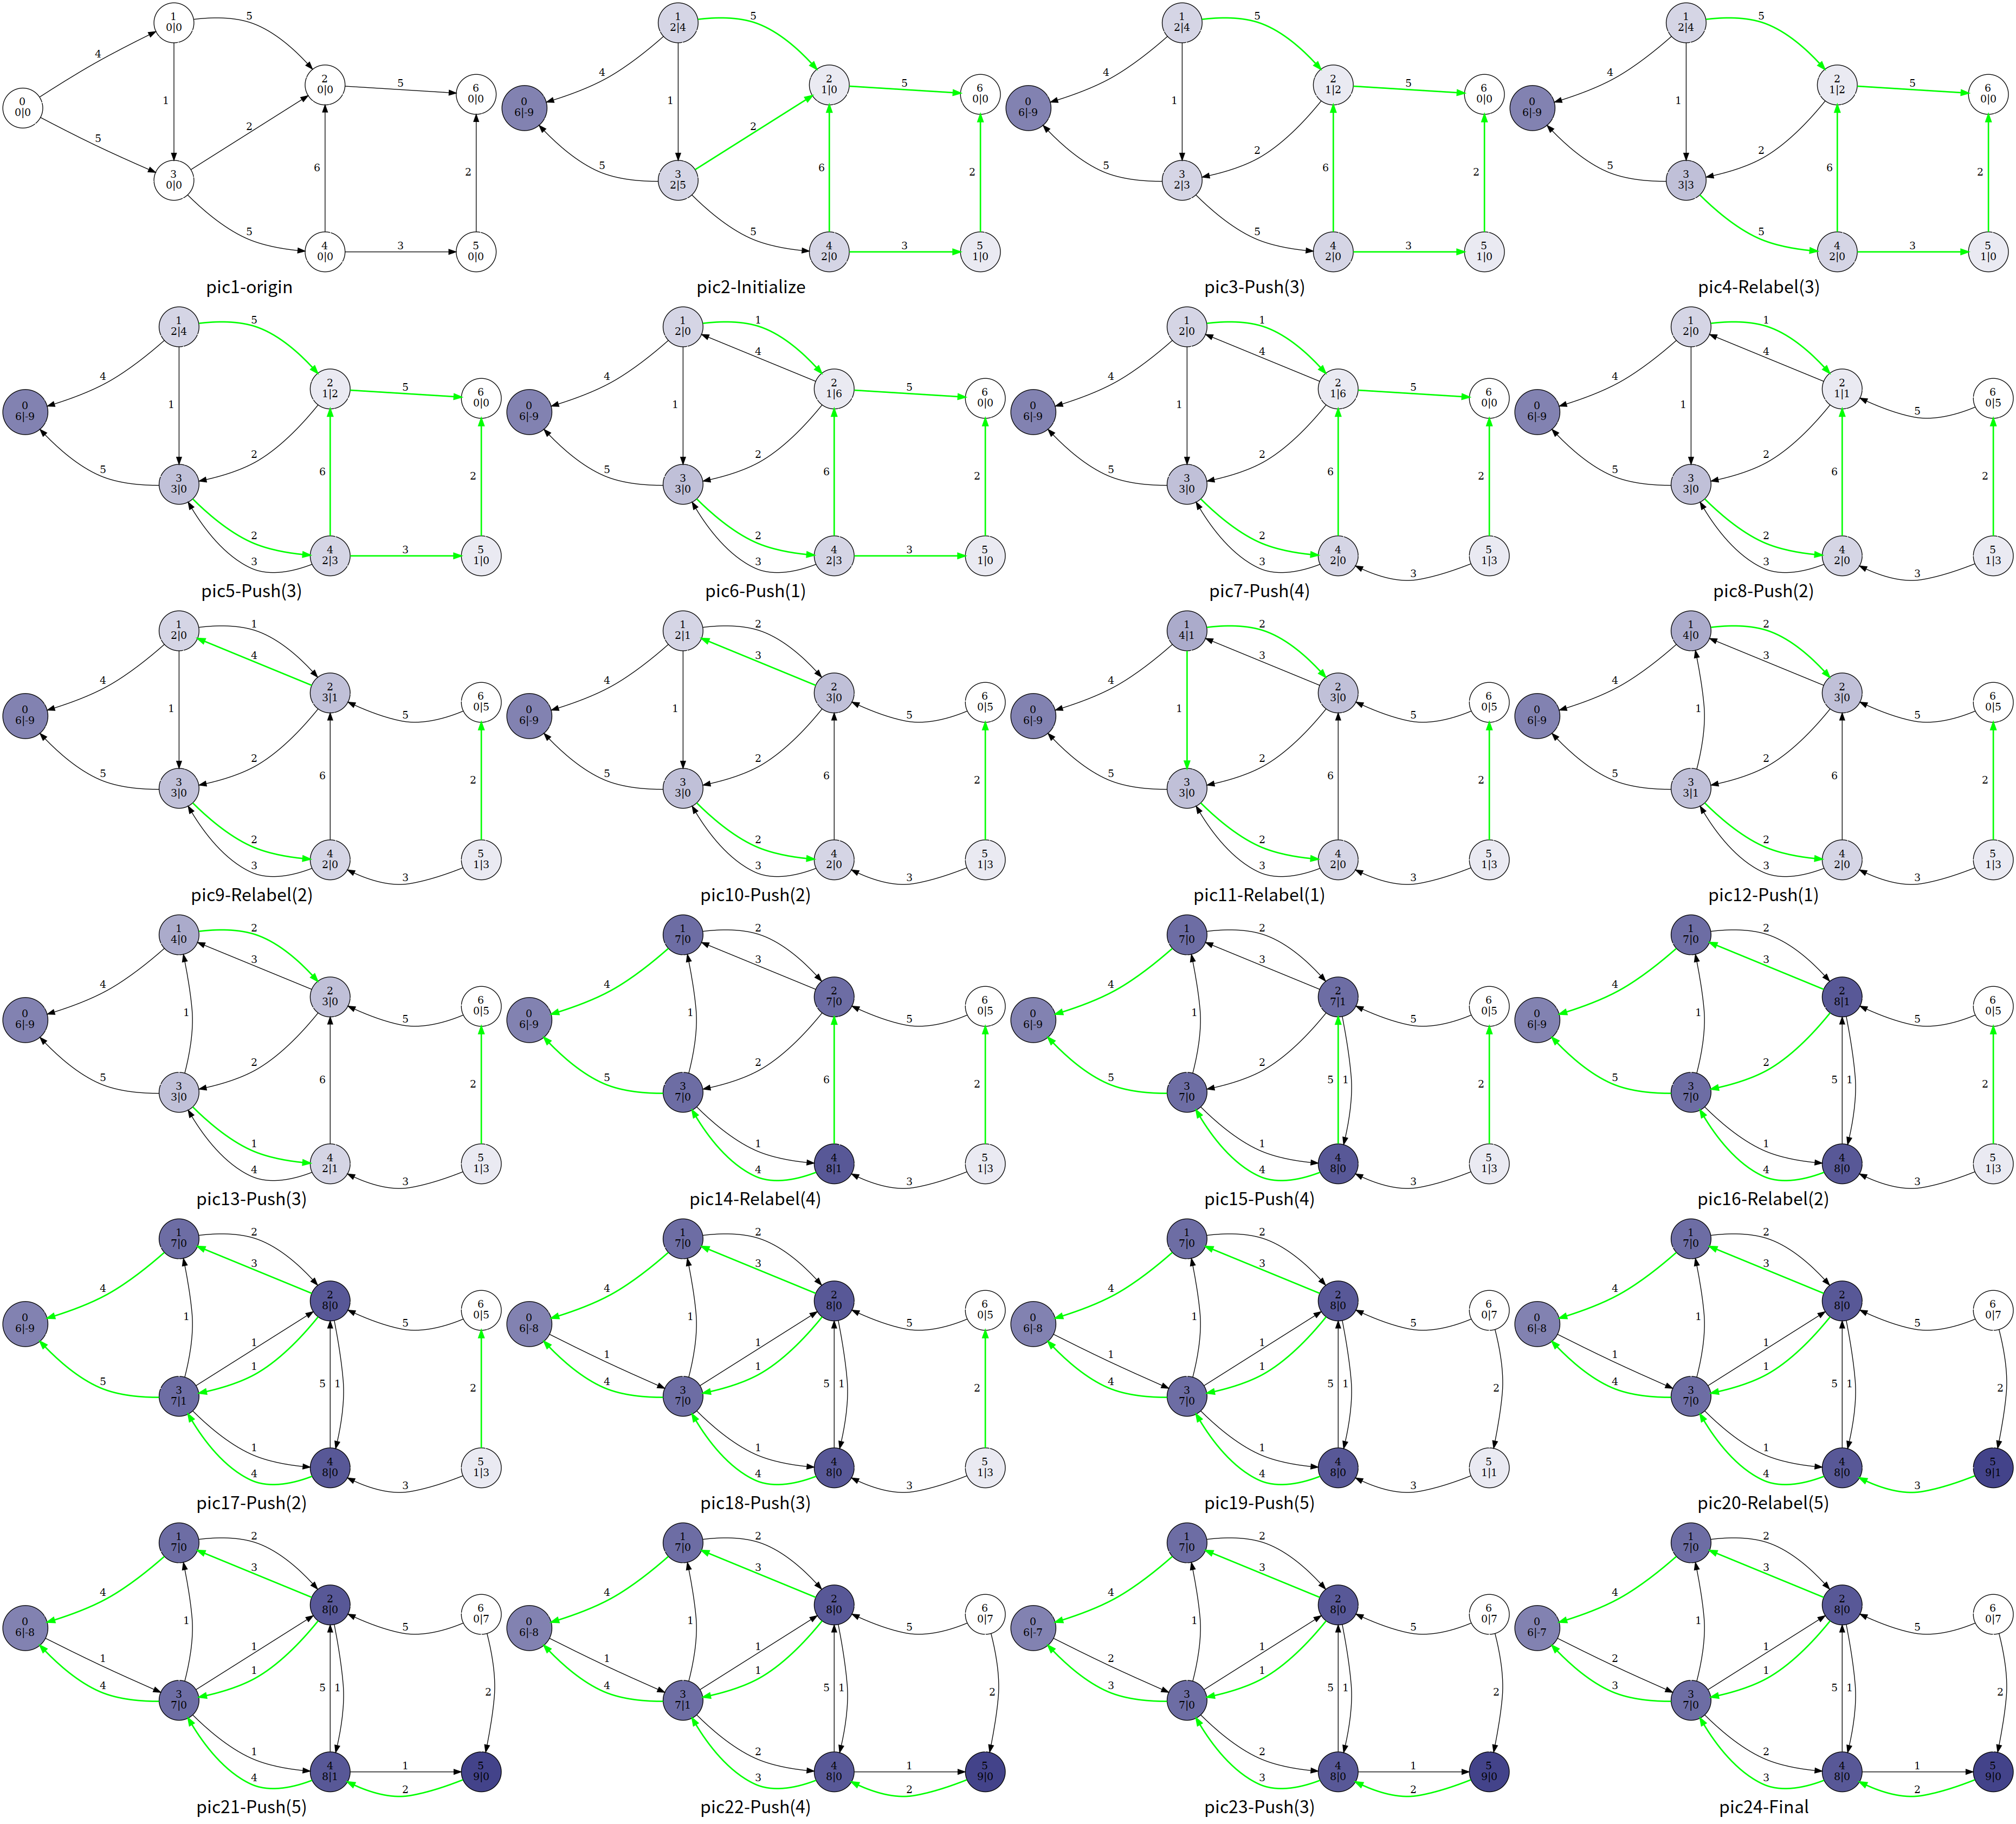
\includegraphics[width=9cm]{graphs/hhlp.png}
\end{center}

\begin{lstlisting}[style=cpp]
struct HLPP {
    int n, m = 0, s, t;
    std::vector<edge> e;      /* 边 */
    std::vector<node> nd;     /* 点 */
    std::vector<int> g[N];    /* 点的连边编号 */
    std::priority_queue<node> q;
    std::queue<int> qq;
    bool vis[N];
    int cnt[N];

    void init() {
        e.clear();
        nd.clear();
        for (int i = 0; i <= n + 1; i++) {
            nd.pushback(node(inf, i, 0));
            g[i].clear();
            vis[i] = false;
        }
    }

    void add(int u, int v, LL w) {
        e.pushback(edge(u, v, w));
        e.pushback(edge(v, u, 0));
        g[u].pushback(m++);
        g[v].pushback(m++);
    }

    void bfs() {
        nd[t].hight = 0;
        qq.push(t);
        while (!qq.empty()) {
            int u = qq.front();
            qq.pop();
            vis[u] = false;
            for (auto j : g[u]) {
                int v = e[j].to;
                if (e[j].cap == 0 && nd[v].hight > nd[u].hight + 1) {
                    nd[v].hight = nd[u].hight + 1;
                    if (vis[v] == false) {
                        qq.push(v);
                        vis[v] = true;
                    }
                }
            }
        }
        return;
    }

    void _push(int u) {
        for (auto j : g[u]) {
            edge &ee = e[j], &er = e[j ^ 1];
            int v = ee.to;
            node &nu = nd[u], &nv = nd[v];
            if (ee.cap && nv.hight + 1 == nu.hight) {
                LL flow = std::min(ee.cap, nu.flow);
                ee.cap -= flow, er.cap += flow;
                nu.flow -= flow, nv.flow += flow;
                if (vis[v] == false && v != t && v != s) {
                    q.push(nv);
                    vis[v] = true;
                }
                if (nu.flow == 0) break;
            }
        }
    }

    void relabel(int u) {
        nd[u].hight = inf;
        for (auto j : g[u]) {
            int v = e[j].to;
            if (e[j].cap && nd[v].hight + 1 < nd[u].hight) {
                nd[u].hight = nd[v].hight + 1;
            }
        }
    }

    LL hlpp() {
        bfs();
        if (nd[s].hight == inf) return 0;
        nd[s].hight = n;
        for (int i = 1; i <= n; i++) {
            if (nd[i].hight < inf) cnt[nd[i].hight]++;
        }
        for (auto j : g[s]) {
            int v = e[j].to;
            int flow = e[j].cap;
            if (flow) {
                e[j].cap -= flow, e[j ^ 1].cap += flow;
                nd[s].flow -= flow, nd[v].flow += flow;
                if (vis[v] == false && v != s && v != t) {
                    q.push(nd[v]);
                    vis[v] = true;
                }
            }
        }
        while (!q.empty()) {
            int u = q.top().id;
            q.pop();
            vis[u] = false;
            _push(u);
            if (nd[u].flow) {
                cnt[nd[u].hight]--;
                if (cnt[nd[u].hight] == 0) {
                    for (int i = 1; i <= n; i++) {
                        if (i != s && i != t && nd[i].hight > nd[u].hight && nd[i].hight < n + 1) {
                            nd[i].hight = n + 1;
                        }
                    }
                }
                relabel(u);
                cnt[nd[u].hight]++;
                q.push(nd[u]);
                vis[u] = true;
            }
        }
        return nd[t].flow;
    }
} maxf;
\end{lstlisting}

\subsection{ network flow - minimum cost flow }
在网络中获得最大流的同时要求费用最小.

\subsubsection*{ Dinic + SPFA }
\begin{lstlisting}[style=cpp]
struct edge {
    int from, to;
    LL cap, cost;

    edge(int u, int v, LL c, LL w) : from(u), to(v), cap(c), cost(w) {}
};

struct MCMF {
    int n, m = 0, s, t;
    std::vector<edge> e;
    vi g[N];
    int cur[N], vis[N];
    LL dist[N], minc;

    void init(int n) {
        for (int i = 0; i < n; i++) g[i].clear();
        e.clear();
        minc = m = 0;
    }

    void add(int from, int to, LL cap, LL cost) {
        e.push_back(edge(from, to, cap, cost));
        e.push_back(edge(to, from, 0, -cost));
        g[from].push_back(m++);
        g[to].push_back(m++);
    }

    bool spfa() {
        rep(i, 1, n) { dist[i] = INF, cur[i] = 0; }
        std::queue<int> q;
        q.push(s), dist[s] = 0, vis[s] = 1;
        while (!q.empty()) {
            int u = q.front();
            q.pop();
            vis[u] = 0;
            for (int j = cur[u]; j < g[u].size(); j++) {
                edge& ee = e[g[u][j]];
                int v = ee.to;
                if (ee.cap && dist[v] > dist[u] + ee.cost) {
                    dist[v] = dist[u] + ee.cost;
                    if (!vis[v]) {
                        q.push(v);
                        vis[v] = 1;
                    }
                }
            }
        }
        return dist[t] != INF;
    }

    LL dfs(int u, LL now) {
        if (u == t) return now;
        vis[u] = 1;
        LL ans = 0;
        for (int& i = cur[u]; i < g[u].size() && ans < now; i++) {
            edge &ee = e[g[u][i]], &er = e[g[u][i] ^ 1];
            int v = ee.to;
            if (!vis[v] && ee.cap && dist[v] == dist[u] + ee.cost) {
                LL f = dfs(v, std::min(ee.cap, now - ans));
                if (f) {
                    minc += f * ee.cost, ans += f;
                    ee.cap -= f;
                    er.cap += f;
                }
            }
        }
        vis[u] = 0;
        return ans;
    }

    PLL mcmf() {
        LL maxf = 0;
        while (spfa()) {
            LL tmp;
            while ((tmp = dfs(s, INF))) maxf += tmp;
        }
        return std::makepair(maxf, minc);
    }
} minc_maxf;
\end{lstlisting}

\subsubsection*{ Primal-Dual 原始对偶算法 }
\begin{lstlisting}[style=cpp]
struct edge {
    int from, to;
    LL cap, cost;

    edge(int u, int v, LL c, LL w) : from(u), to(v), cap(c), cost(w) {}
};

struct node {
    int v, e;

    node(int _v = 0, int _e = 0) : v(_v), e(_e) {}
};

const int maxn = 5000 + 10;

struct MCMF {
    int n, m = 0, s, t;
    std::vector<edge> e;
    vi g[maxn];
    int dis[maxn], vis[maxn], h[maxn];
    node p[maxn * 2];

    void add(int from, int to, LL cap, LL cost) {
        e.push_back(edge(from, to, cap, cost));
        e.push_back(edge(to, from, 0, -cost));
        g[from].push_back(m++);
        g[to].push_back(m++);
    }

    bool dijkstra() {
        std::priority_queue<PII, std::vector<PII>, std::greater<PII>> q;
        for (int i = 1; i <= n; i++) {
            dis[i] = inf;
            vis[i] = 0;
        }
        dis[s] = 0;
        q.push({0, s});
        while (!q.empty()) {
            int u = q.top().ss;
            q.pop();
            if (vis[u]) continue;
            vis[u] = 1;
            for (auto i : g[u]) {
                edge ee = e[i];
                int v = ee.to, nc = ee.cost + h[u] - h[v];
                if (ee.cap and dis[v] > dis[u] + nc) {
                    dis[v] = dis[u] + nc;
                    p[v] = node(u, i);
                    if (!vis[v]) q.push({dis[v], v});
                }
            }
        }
        return dis[t] != inf;
    }

    void spfa() {
        std::queue<int> q;
        for (int i = 1; i <= n; i++) h[i] = inf;
        h[s] = 0, vis[s] = 1;
        q.push(s);
        while (!q.empty()) {
            int u = q.front();
            q.pop();
            vis[u] = 0;
            for (auto i : g[u]) {
                edge ee = e[i];
                int v = ee.to;
                if (ee.cap and h[v] > h[u] + ee.cost) {
                    h[v] = h[u] + ee.cost;
                    if (!vis[v]) {
                        vis[v] = 1;
                        q.push(v);
                    }
                }
            }
        }
    }

    PLL mcmf() {
        LL maxf = 0, minc = 0;
        spfa();
        while (dijkstra()) {
            LL minf = INF;
            for (int i = 1; i <= n; i++) h[i] += dis[i];
            for (int i = t; i != s; i = p[i].v) minf = std::min(minf, e[p[i].e].cap);
            for (int i = t; i != s; i = p[i].v) {
                e[p[i].e].cap -= minf;
                e[p[i].e ^ 1].cap += minf;
            }
            maxf += minf;
            minc += minf * h[t];
        }
        return std::make_pair(maxf, minc);
    }
} minc_maxf;
\end{lstlisting}

\subsubsection*{ 存在负环的网络 }

\subsection{ network flow - minimal cut }
最小割解决的问题是将图中的点集 \(V\) 划分成 \(S\) 与 \(T\), 使得 \(S\) 与 \(T\) 之间的连边的容量总和最小.

\subsubsection*{ 最大流最小割定理 }
网络中 \(s\) 到 \(t\) 的最大流流量的值等于所要求的最小割的值, 所以求最小割只需要跑 Dinic 即可.

\subsubsection*{ 获得 \(S\) 中的所有点 }
在 Dinic 的 \(\operatorname{bfs}\) 函数中, 每次将所有点的 \(d\) 数组值改为无穷大, 最后跑完最大流之后 \(d\) 数组不为无穷大的就是和源点一起在 \(S\) 集合中的点.

\subsubsection*{ 例子 }
最小割的本质是对图中点集进行 \(2\)-划分, 网络流只是求解答案的手段.
\begin{enumerate}
	\item 在图中花费最小的代价断开一些边使得源点 \(s\) 无法流到汇点 \(t\).

    直接跑最大流就得到了答案.
    \item 在图中删除最少的点使得源点 \(s\) 无法流到汇点 \(t\).

    对每个点进行拆点, 在 \(i\) 与 \(i^\prime\) 之间建立容量为 \(1\) 的有向边.
\end{enumerate}

\subsection{ matching - matching on bipartite graph }
\subsubsection*{ 二分图最大匹配 }
\subsubsection*{ Kuhn-Munkres }
时间复杂度: \(O(n^3)\).

\begin{lstlisting}[style=cpp]
auto KM = [&](int n1, int n2, vvi e) -> std::pair<vi, vi> {
    vi vis(n2 + 1);
    vi l(n1 + 1, -1), r(n2 + 1, -1);
    std::function<bool(int)> dfs = [&](int u) -> bool {
        for (auto v : e[u]) {
            if (!vis[v]) {
                vis[v] = 1;
                if (r[v] == -1 or dfs(r[v])) {
                    r[v] = u;
                    return true;
                }
            }
        }
        return false;
    };
    for (int i = 1; i <= n1; i++) {
        std::fill(all(vis), 0);
        dfs(i);
    }
    for (int i = 1; i <= n2; i++) {
        if (r[i] == -1) continue;
        l[r[i]] = i;
    }
    return {l, r};
};
auto [mchl, mchr] = KM(n1, n2, e);
std::cout << mchl.size() - std::count(all(mchl), -1) << endl;
\end{lstlisting}

\subsubsection*{ Hopcroft-Karp }
据说时间复杂度是 \(O(m \sqrt{n})\) 的, 但是快的飞起.

\begin{lstlisting}[style=cpp]
vpi e(m);
auto hopcroft_karp = [&](int n, int m, vpi& e) -> std::pair<vi, vi> {
    vi g(e.size()), l(n + 1, -1), r(m + 1, -1), d(n + 2);
    for (auto [u, v] : e) d[u]++;
    std::partial_sum(all(d), d.begin());
    for (auto [u, v] : e) g[--d[u]] = v;
    for (vi a, p, q(n + 1);;) {
        a.assign(n + 1, -1);
        p.assign(n + 1, -1);
        int t = 1;
        for (int i = 1; i <= n; i++) {
            if (l[i] == -1) {
                q[t++] = a[i] = p[i] = i;
            }
        }
        bool match = false;
        for (int i = 1; i < t; i++) {
            int u = q[i];
            if (l[a[u]] != -1) continue;
            for (int j = d[u]; j < d[u + 1]; j++) {
                int v = g[j];
                if (r[v] == -1) {
                    while (v != -1) {
                        r[v] = u;
                        std::swap(l[u], v);
                        u = p[u];
                    }
                    match = true;
                    break;
                }
                if (p[r[v]] == -1) {
                    q[t++] = v = r[v];
                    p[v] = u;
                    a[v] = a[u];
                }
            }
        }
        if (!match) break;
    }
    return {l, r};
};
\end{lstlisting}

\subsubsection*{ 二分图最大权匹配 }
\subsubsection*{ Kuhn-Munkres }
注意是否为完美匹配, 非完美选 \(0\), 完美选 \(-INF\). (存疑)

\begin{lstlisting}[style=cpp]
auto KM = [&](int n, vvl e) -> std::tuple<LL, vi, vi> {
    vl la(n + 1), lb(n + 1), pp(n + 1), vx(n + 1);
    vi l(n + 1, -1), r(n + 1, -1);
    vi va(n + 1), vb(n + 1);
    LL delta;
    auto bfs = [&](int x) -> void {
        int a, y = 0, y1 = 0;
        std::fill(all(pp), 0);
        std::fill(all(vx), INF);
        r[y] = x;
        do {
            a = r[y], delta = INF, vb[y] = 1;
            for (int b = 1; b <= n; b++) {
                if (!vb[b]) {
                    if (vx[b] > la[a] + lb[b] - e[a][b]) {
                        vx[b] = la[a] + lb[b] - e[a][b];
                        pp[b] = y;
                    }
                    if (vx[b] < delta) {
                        delta = vx[b];
                        y1 = b;
                    }
                }
            }
            for (int b = 0; b <= n; b++) {
                if (vb[b]) {
                    la[r[b]] -= delta;
                    lb[b] += delta;
                } else
                    vx[b] -= delta;
            }
            y = y1;
        } while (r[y] != -1);
        while (y) {
            r[y] = r[pp[y]];
            y = pp[y];
        }
    };
    for (int i = 1; i <= n; i++) {
        std::fill(all(vb), 0);
        bfs(i);
    }
    LL ans = 0;
    for (int i = 1; i <= n; i++) {
        if (r[i] == -1) continue;
        l[r[i]] = i;
        ans += e[r[i]][i];
    }
    return {ans, l, r};
};

auto [ans, mchl, mchr] = KM(n, e);
\end{lstlisting}

\subsection{ matching - matching on general graph }

\newpage
\section{ geometry }
\subsection{ two demention }
\subsubsection*{ 点与向量 }
\begin{lstlisting}[style=cpp]
tandu struct pnt {
    T x, y;

    pnt(T _x = 0, T _y = 0) { x = _x, y = _y; }

    pnt operator+(const pnt& a) const { return pnt(x + a.x, y + a.y); }

    pnt operator-(const pnt& a) const { return pnt(x - a.x, y - a.y); }

    /*
    bool operator<(const pnt& a) const {
        if (std::is_same<T, double>::value) {
            if (fabs(x - a.x) < eps) return y < a.y;
        } else {
            if (x == a.x) return y < a.y;
        }
        return x < a.x;
    }
    */

    /* 注意数乘会不会爆 int */
    pnt operator*(const T k) const { return pnt(k * x, k * y); }

    U operator*(const pnt& a) const { return (U) x * a.x + (U) y * a.y; }

    U operator^(const pnt& a) const { return (U) x * a.y - (U) y * a.x; }

    U dist(const pnt a) { return ((U) a.x - x) * ((U) a.x - x) + ((U) a.y - y) * ((U) a.y - y); }

    U len() { return dist(pnt(0, 0)); }

    /* a, b, c 成逆时针 */
    friend U area(pnt a, pnt b, pnt c) { return (b - a) ^ (c - a); }

    /* 两向量夹角,返回 cos 值 */
    double get_angle(pnt a) {
        return (double) (pnt(x, y) * a) / sqrt((double) pnt(x, y).len() * (double) a.len());
    }
};
\end{lstlisting}

\subsubsection*{ 线段 }

\begin{lstlisting}[style=cpp]
struct line {
    point a, b;

    line(point _a = {}, point _b = {}) { a = _a, b = _b; }

    /* 交点类型为 double */
    friend point iPoint(line p, line q) {
        point v1 = p.b - p.a;
        point v2 = q.b - q.a;
        point u = q.a - p.a;
        return q.a + (q.b - q.a) * ((u ^ v1) * 1. / (v1 ^ v2));
    }

    /* 极角排序 */
    bool operator<(const line& p) const {
        double t1 = std::atan2((b - a).y, (b - a).x);
        double t2 = std::atan2((p.b - p.a).y, (p.b - p.a).x);
        if (fabs(t1 - t2) > eps) {
            return t1 < t2;
        }
        return ((p.a - a) ^ (p.b - a)) > eps;
    }
};
\end{lstlisting}

\subsection{ convex }
\subsubsection*{ 2D }
\begin{lstlisting}[style=cpp]
auto andrew = [&](std::vector<point>& v) -> std::vector<point> {
    std::sort(all(v));
    std::vector<point> stk;
    for (int i = 0; i < n; i++) {
        point x = v[i];
        while (stk.size() > 1 and ((stk.end()[-1] - stk.end()[-2]) ^ (x - stk.end()[-2])) <= 0) {
            stk.pop_back();
        }
        stk.push_back(x);
    }
    int tmp = stk.size();
    for (int i = n - 2; i >= 0; i--) {
        point x = v[i];
        while (stk.size() > tmp and ((stk.end()[-1] - stk.end()[-2]) ^ (x - stk.end()[-2])) <= 0) {
            stk.pop_back();
        }
        stk.push_back(x);
    }
    return stk;
};
\end{lstlisting}

\subsection*{ 旋转卡壳 }
\begin{lstlisting}[style=cpp]
#include<cstdio>
#include<algorithm>
#define db double
namespace Acc{
    const int N = 5e4+10;
    struct node{
        int x,y;
    }a[N],stk[N];
    db cmp(node a,node b,node c){return 1.*(c.x-a.x)*(c.y-b.y)-1.*(c.x-b.x)*(c.y-a.y);}
    int dis(node a,node b){return ((a.x-b.x)*(a.x-b.x)+(a.y-b.y)*(a.y-b.y));}
    int n,tp,ans;
    void work(){
        scanf("%d",&n);
        for(int i=1;i<=n;i++)scanf("%d%d",&a[i].x,&a[i].y);
        std::sort(a+1,a+n+1,[=](node a,node b)->bool{return a.x<b.x || (a.x==b.x && a.y<b.y);});
        stk[1]=a[1],tp=1;
        for(int i=2;i<=n;i++){
            while(tp>1 && cmp(stk[tp-1],stk[tp],a[i])<=0)tp--;
            stk[++tp]=a[i];
        }
        int tmp=tp;
        for(int i=n-1;i>=1;i--){
            while(tp>tmp && cmp(stk[tp-1],stk[tp],a[i])<=0)tp--;
            stk[++tp]=a[i];
        }
        for(int i=1,j=3;i<tp;i++){
            while(cmp(stk[i],stk[i+1],stk[j])<cmp(stk[i],stk[i+1],stk[j+1]))j=j%(tp-1)+1;
            ans=std::max(ans,std::max(dis(stk[i],stk[j]),dis(stk[i+1],stk[j])));
        }
        printf("%d",ans);
    }
}
int main(){
    return Acc::work(),0;
}
\end{lstlisting}

\subsection*{ half plane }
\begin{lstlisting}[style=cpp]
auto halfPlane = [&](std::vector<line>& ln) -> std::vector<point> {
    std::sort(all(ln));
    ln.erase(
        unique(
            all(ln),
            [](line& p, line& q) {
                double t1 = std::atan2((p.b - p.a).y, (p.b - p.a).x);
                double t2 = std::atan2((q.b - q.a).y, (q.b - q.a).x);
                return fabs((t1 - t2)) < eps;
            }),
        ln.end());
    auto check = [&](line p, line q, line r) -> bool {
        point a = iPoint(p, q);
        return ((r.b - r.a) ^ (a - r.a)) < -eps;
    };
    line q[ln.size() + 2];
    int hh = 1, tt = 0;
    q[++tt] = ln[0];
    q[++tt] = ln[1];
    for (int i = 2; i < (int) ln.size(); i++) {
        while (hh < tt and check(q[tt - 1], q[tt], ln[i])) tt--;
        while (hh < tt and check(q[hh + 1], q[hh], ln[i])) hh++;
        q[++tt] = ln[i];
    }
    while (hh < tt and check(q[tt - 1], q[tt], q[hh])) tt--;
    while (hh < tt and check(q[hh + 1], q[hh], q[tt])) hh++;
    q[tt + 1] = q[hh];
    std::vector<point> ans;
    for (int i = hh; i <= tt; i++) {
        ans.push_back(iPoint(q[i], q[i + 1]));
    }
    return ans;
};
\end{lstlisting}

\section{ sweep line }

矩形面积并

\begin{lstlisting}[style=cpp]
#define int long long
const int N = 2e5+10;
int b[N<<1],n,len,ans;
struct node{
    int y1,y2,x,k;
}a[N<<1];
struct Seg{
#define lc (o<<1)
#define rc (o<<1|1)
    static const int N = 5e6+10;
    int sum[N],cnt[N],tag[N];
    void push_up(int o,int l,int r){
        if(sum[o])cnt[o]=b[r+1]-b[l];
        else cnt[o]=cnt[lc]+cnt[rc];
    }
    void add(int o,int l,int r,int L,int R,int k){
        if(r<L || l>R)return;
        if(l==L && r==R)return (void)(sum[o]+=k,push_up(o,l,r));
        int mid=L+R>>1;
        if(r<=mid)add(lc,l,r,L,mid,k);
        else if(l>mid)add(rc,l,r,mid+1,R,k);
        else add(lc,l,mid,L,mid,k),add(rc,mid+1,r,mid+1,R,k);
        push_up(o,L,R);
    }
#undef lc
#undef rc
}t;
void work(){
    cin>>n;
    for(int i=1,x1,y1,x2,y2;i<=n;i++){
        cin>>x1>>y1>>x2>>y2;
        b[i*2-1]=y1,b[i*2]=y2,a[i*2-1]={y1,y2,x1,1},a[i*2]={y1,y2,x2,-1};
    }
    n<<=1;
    sort(b+1,b+n+1),len=unique(b+1,b+n+1)-b-1;
    for(int i=1;i<=n;i++)a[i].y1=lower_bound(b+1,b+len+1,a[i].y1)-b,a[i].y2=lower_bound(b+1,b+len+1,a[i].y2)-b;
    sort(a+1,a+n+1,[](node a,node b)->bool{return a.x<b.x;});
    for(int i=1;i<n;i++){
        t.add(1,a[i].y1,a[i].y2-1,1,len-1,a[i].k);
        ans+=t.cnt[1]*(a[i+1].x-a[i].x);
    }
    cout<<ans;
}
#undef int
\end{lstlisting}

\newpage
\section{ offline algorithm}
\subsection{ discretization }
\begin{lstlisting}[style=cpp]
std::sort(all(a));
a.erase(unique(all(a)), a.end());
auto get_id = [&](const int& x) -> int { return lower_bound(all(a), x) - a.begin() + 1; };
\end{lstlisting}

\subsection{ Mo algorithm }
\subsubsection*{ 普通莫队 }
\begin{lstlisting}[style=cpp]
int block = n / sqrt(2 * m / 3);
std::sort(all(q), [&](node a, node b) {
    return a.l / block == b.l / block ? (a.r == b.r ? 0 : ((a.l / block) & 1) ^ (a.r < b.r))
                                        : a.l < b.l;
});

auto move = [&](int x, int op) -> void {
    if (op == 1) {
        /* operations */
    } else {
        /* operations */
    }
};

for (int k = 1, l = 1, r = 0; k <= m; k++) {
    node Q = q[k];
    while (l > Q.l) {
        move(--l, 1);
    }
    while (r < Q.r) {
        move(++r, 1);
    }
    while (l < Q.l) {
        move(l++, -1);
    }
    while (r > Q.r) {
        move(r--, -1);
    }
}
\end{lstlisting}

\subsubsection*{ 回滚莫队 }

例题:P5906 给定一个序列,多次询问一个区间中相同数的最远间隔距离.

\begin{lstlisting}[style = cpp]
#include<bits/stdc++.h>
namespace Acc {
    const int N = 200009;
    int a[N], b[N], id[N], f[N], g[N], p[N], z[N];
    std::pair<int, int> st[N];
    struct T {
        int l, r, o;
    }q[N];
    auto work = []() {
        int n, m;
        std::cin >> n;
        for (int i = 1; i <= n; ++i) {
            std::cin >> a[i], b[i] = a[i];
        }
        std::sort(b + 1, b + n + 1);
        int ct = std::unique(b + 1, b + n + 1) - b - 1;
        for (int i = 1; i <= n; ++i) {
            a[i] = std::lower_bound(b + 1, b + ct + 1, a[i]) - b;
        }
        std::cin >> m;
        for (int i = 1; i <= m; ++i) {
            auto&[l, r, o] = q[i];
            std::cin >> l >> r, o = i;
        }
        int B = ceil(n / sqrt(m));
        for (int i = 1; i <= n; ++i) {
            id[i] = (i - 1) / B + 1;
        }
        std::sort(q + 1, q + m + 1, [](T a, T b) {
            return id[a.l] == id[b.l] ? a.r < b.r : a.l < b.l;
        });
        int ans = 0, L = 1, R = 0;
        for (int i = 1; i <= m; ++i) {
            auto[l, r, o] = q[i];
            if (id[l] != id[q[i - 1].l]) {
                ans = 0;
                R = std::min(n, id[l] * B), L = R + 1;
                memset(f + 1, 0, ct << 2);
                memset(g + 1, 0, ct << 2);
            }
            if (id[l] == id[r]) {
                for (int j = l; j <= r; ++j) {
                    if (p[a[j]] == 0) p[a[j]] = j;
                    else ans = std::max(ans, j - p[a[j]]);
                }
                for (int j = l; j <= r; ++j) p[a[j]] = 0;
                z[o] = ans, ans = 0;
            } else {
                while (R < r) {
                    ++R, g[a[R]] = R;
                    if (f[a[R]] == 0) f[a[R]] = R;
                    else ans = std::max(ans, R - f[a[R]]);
                }
                int las = ans, t = L;
                while (l < L) {
                    --L;
                    int x = f[a[L]], y = g[a[L]];
                    st[L] = std::make_pair(x, y);
                    f[a[L]] = L;
                    if (g[a[L]] == 0) g[a[L]] = L;
                    else ans = std::max(ans, g[a[L]] - L);
                }
                z[o] = ans;
                for (int j = l; j < t; ++j) {
                    auto[x, y] = st[j];
                    f[a[j]] = x, g[a[j]] = y;
                }
                ans = las, L = t;
            }
        }
        for (int i = 1; i <= m; ++i) {
            std::cout << z[i] << '\n';
        }
    };
}
int main() {
    std::ios::sync_with_stdio(0);
    std::cin.tie(0), Acc::work();
}
\end{lstlisting}

\subsection{ CDQ }

\(n\) 个三维数对 \((a_i, b_i, c_i)\), 设 \(f(i)\) 表示 \(a_j \leqslant a_i, b_j \leqslant b_i, c_j \leqslant c_i (i \neq j)\) 的个数.
输出 \(f(i) \ (0 \leqslant i \leqslant n - 1)\) 的值.

\begin{lstlisting}[style=cpp]
// 洛谷 P3810 【模板】三维偏序(陌上花开)

struct data {
    int a, b, c, cnt, ans;

    data(int _a = 0, int _b = 0, int _c = 0, int _cnt = 0, int _ans = 0) {
        a = _a, b = _b, c = _c, cnt = _cnt, ans = _ans;
    }

    bool operator!=(data x) {
        if (a != x.a) return true;
        if (b != x.b) return true;
        if (c != x.c) return true;
        return false;
    }
};

int main() {
    std::ios::sync_with_stdio(false);
    std::cin.tie(0);
    std::cout.tie(0);


    int n, k;
    std::cin >> n >> k;
    static data v1[N], v2[N];
    for (int i = 1; i <= n; i++) {
        std::cin >> v1[i].a >> v1[i].b >> v1[i].c;
    }

    std::sort(v1 + 1, v1 + n + 1, [&](data x, data y) {
        if (x.a != y.a) return x.a < y.a;
        if (x.b != y.b) return x.b < y.b;
        return x.c < y.c;
    });

    int t = 0, top = 0;
    for (int i = 1; i <= n; i++) {
        t++;
        if (v1[i] != v1[i + 1]) {
            v2[++top] = v1[i];
            v2[top].cnt = t;
            t = 0;
        }
    }

    vi tr(N);

    auto add = [&](int pos, int val) -> void {
        while (pos <= k) {
            tr[pos] += val;
            pos += lowbit(pos);
        }
    };

    auto query = [&](int pos) -> int {
        int ans = 0;
        while (pos > 0) {
            ans += tr[pos];
            pos -= lowbit(pos);
        }
        return ans;
    };

    std::function<void(int, int)> CDQ = [&](int l, int r) -> void {
        if (l == r) return;
        int mid = (l + r) >> 1;
        CDQ(l, mid), CDQ(mid + 1, r);
        std::sort(v2 + l, v2 + mid + 1, [&](data x, data y) {
            if (x.b != y.b) return x.b < y.b;
            return x.c < y.c;
        });
        std::sort(v2 + mid + 1, v2 + r + 1, [&](data x, data y) {
            if (x.b != y.b) return x.b < y.b;
            return x.c < y.c;
        });
        int i = l, j = mid + 1;
        while (j <= r) {
            while (i <= mid && v2[i].b <= v2[j].b) {
                add(v2[i].c, v2[i].cnt);
                i++;
            }
            v2[j].ans += query(v2[j].c);
            j++;
        }
        for (int ii = l; ii < i; ii++) {
            add(v2[ii].c, -v2[ii].cnt);
        }
        return;
    };

    CDQ(1, top);
    vi ans(n + 1);
    for (int i = 1; i <= top; i++) {
        ans[v2[i].ans + v2[i].cnt] += v2[i].cnt;
    }
    for (int i = 1; i <= n; i++) {
        std::cout << ans[i] << endl;
    }

    return 0;
}
\end{lstlisting}

\begin{lstlisting}[style = cpp]
#include<bits/stdc++.h>
using namespace std;
namespace Acc {
    const int N = 2e5 + 9;
    struct T {
        int x, y, z, o;
        bool operator==(const T& b) const {
            return x == b.x && y == b.y && z == b.z;
        }
        bool operator<(const T& b) const {
            if (x != b.x) return x < b.x;
            if (y != b.y) return y < b.y;
            return z < b.z;
        }
    }a[N];
    long long z[N];
    int m, t[N], f[N];
    auto ins = [](int x, int k) {
        for (; x <= m; x += x & -x) t[x] += k;
    };
    auto ask = [](int x) {
        int z = 0;
        for (; x; x ^= x & -x) z += t[x];
        return z;
    };
    void CDQ(int l, int r) {
        if (l == r) return ;
        int md = l + r >> 1;
        CDQ(l, md), CDQ(md + 1, r);
        int i, j;
        for (i = l, j = md + 1; j <= r; ++j) {
            for (; i <= md && a[i].y <= a[j].y; ++i) ins(a[i].z, 1);
            f[a[j].o] += ask(a[j].z);
        }
        for (--i; i >= l; --i) ins(a[i].z, -1);
        inplace_merge(a + l, a + md + 1, a + r + 1, [](T a, T b) {
            return a.y < b.y;
        });
    }
    auto work = []() {
        int n;
        cin >> n >> m;
        for (int i = 1; i <= n; ++i) {
            auto&[x, y, z, o] = a[i];
            cin >> x >> y >> z;
        }
        sort(a + 1, a + n + 1);
        for (int i = 1; i <= n; ++i) a[i].o = i;
        CDQ(1, n);
        sort(a + 1, a + n + 1);
        for (int i = n - 1; i; --i) {
            if (a[i] == a[i + 1]) f[i] = f[i + 1];
        }
        for (int i = 1; i <= n; ++i) ++z[f[i]];
        for (int i = 0; i < n; ++i) cout << z[i] << '\n';
    };
}
int main() {
    ios::sync_with_stdio(0);
    cin.tie(0), Acc::work();
}
\end{lstlisting}

\subsection{ 线段树分治 }
\begin{lstlisting}[style=cpp]
#include<bits/stdc++.h>
using namespace std;
namespace Acc {
    const int N = 1e5;
    pair<int, int> q[N * 2];
    vector<int> v[N * 4];
    int n, l, r, p;
    int fa[N * 2], sz[N * 2];
    pair<int, int> st[N * 2];
    int tp;
    void ins(int o, int L, int R) {
        if (r < L || l > R) return ;
        if (l <= L && R <= r) {
            v[o].emplace_back(p);
            return ;
        }
        int md = L + R >> 1;
        ins(o << 1, L, md);
        ins(o << 1 | 1, md + 1, R);
    }
    auto gf = [](int x) {
        while (x != fa[x]) x = fa[x];
        return x;
    };
    auto mg = [](int x, int y) {
        x = gf(x), y = gf(y);
        if (x != y) {
            if (sz[x] < sz[y]) swap(x, y);
            fa[y] = x, sz[x] += sz[y];
            st[++tp] = {x, y};
        }
    };
    void dfs(int o, int L, int R) {
        int lastp = tp;
        for (int i : v[o]) {
            auto[x, y] = q[i];
            mg(x, y + n), mg(x + n, y);
            if (gf(x) == gf(x + n)) {
                for (int i = L; i <= R; ++i) {
                    cout << "No\n";
                }
                goto _;
            }
        }
        if (L == R) {
            cout << "Yes\n";
        } else {
            int md = L + R >> 1;
            dfs(o << 1, L, md);
            dfs(o << 1 | 1, md + 1, R);
        }
        _:
        for (; tp > lastp; --tp) {
            auto[x, y] = st[tp];
            fa[y] = y, sz[x] -= sz[y];
        }
    }
    auto work = []() {
        int m, k;
        cin >> n >> m >> k;
        for (int i = 1; i <= m; ++i) {
            int x, y;
            cin >> x >> y >> l >> r;
            if (++l <= r) {
                q[p = i] = {x, y}, ins(1, 1, k);
            }
        }
        iota(fa + 1, fa + n * 2 + 1, 1);
        fill(sz + 1, sz + n * 2 + 1, 1);
        dfs(1, 1, k);
    };
}
int main() {
    ios::sync_with_stdio(0);
    cin.tie(0), Acc::work();
}
\end{lstlisting}

\end{document}
